\documentclass[letterpaper]{article}
\usepackage[margin=1in]{geometry}
\usepackage[utf8]{inputenc}
\usepackage{textcomp}
\usepackage{amssymb}
\usepackage{natbib}
\usepackage{graphicx}
\usepackage{gensymb}
\usepackage{amsthm, amsmath, mathtools}
\usepackage[dvipsnames]{xcolor}
\usepackage{enumerate}
\usepackage{mdframed}
\usepackage[most]{tcolorbox}
\usepackage{csquotes}
% https://tex.stackexchange.com/questions/13506/how-to-continue-the-framed-text-box-on-multiple-pages

\tcbuselibrary{theorems}

\newcommand{\R}{\mathbb{R}}
\newcommand{\Z}{\mathbb{Z}}
\newcommand{\N}{\mathbb{N}}
\newcommand{\Q}{\mathbb{Q}}
\newcommand{\C}{\mathbb{C}}
\newcommand{\code}[1]{\texttt{#1}}
\newcommand{\mdiamond}{$\diamondsuit$}
\newcommand{\PowerSet}{\mathcal{P}}
\newcommand{\Mod}[1]{\ (\mathrm{mod}\ #1)}
\DeclareMathOperator{\lcm}{lcm}

%\newtheorem*{theorem}{Theorem}
%\newtheorem*{definition}{Definition}
%\newtheorem*{corollary}{Corollary}
%\newtheorem*{lemma}{Lemma}
\newtheorem*{proposition}{Proposition}


\newtcbtheorem[number within=section]{theorem}{Theorem}
{colback=green!5,colframe=green!35!black,fonttitle=\bfseries}{th}

\newtcbtheorem[number within=section]{definition}{Definition}
{colback=blue!5,colframe=blue!35!black,fonttitle=\bfseries}{def}

\newtcbtheorem[number within=section]{corollary}{Corollary}
{colback=yellow!5,colframe=yellow!35!black,fonttitle=\bfseries}{cor}

\newtcbtheorem[number within=section]{lemma}{Lemma}
{colback=red!5,colframe=red!35!black,fonttitle=\bfseries}{lem}

\newtcbtheorem[number within=section]{example}{Example}
{colback=white!5,colframe=white!35!black,fonttitle=\bfseries}{def}

\newtcbtheorem[number within=section]{note}{Important Note}{
        enhanced,
        sharp corners,
        attach boxed title to top left={
            xshift=-1mm,
            yshift=-5mm,
            yshifttext=-1mm
        },
        top=1.5em,
        colback=white,
        colframe=black,
        fonttitle=\bfseries,
        boxed title style={
            sharp corners,
            size=small,
            colback=red!75!black,
            colframe=red!75!black,
        } 
    }{impnote}
\usepackage[utf8]{inputenc}
\usepackage[english]{babel}
\usepackage{fancyhdr}
\usepackage[hidelinks]{hyperref}

\pagestyle{fancy}
\fancyhf{}
\rhead{Math 100A}
\chead{December 1st, 2021}
\lhead{Course Notes}
\rfoot{\thepage}

\setlength{\parindent}{0pt}

\begin{document}

\begin{titlepage}
    \begin{center}
        \vspace*{1cm}
            
        \Huge
        \textbf{Math 100A Notes}
            
        \vspace{0.5cm}
        \LARGE
        Abstract Algebra: Group Theory
            
        \vspace{1.5cm}
            
        \vfill
            
        Fall 2021\\
        Taught by Professor Kiran Kedlaya
    \end{center}
\end{titlepage}

\pagenumbering{gobble}

\newpage 

\pagenumbering{gobble}
\begingroup
    \renewcommand\contentsname{Table of Contents}
    \tableofcontents
\endgroup

\newpage
\pagenumbering{arabic}

\section{Introduction to Binary Operations}
We want to explore the idea behind \emph{algebraic structures}. In particular, we want to explore these structures in more detail compared to earlier courses (either in past college or high school algebra classes). 


\bigskip 

To do this, we need to think about \emph{what} algebra really is. We might think about solving equations like $x^2 + 3x + 5 = 0$ for $x$. In particular, what is really happening here?

\bigskip 

Well, there are a couple of operations going on. Specifically, we have \emph{addition} and \emph{multiplication}. 
\[x \times x + 3 \times x + 5 = 0\]
We now want to examine these operations. Both of these operations $(+, \times)$ take in \underline{two numbers} and output \underline{one number}. The question we might have, then, is: how can we can generalize these operations?


\subsection{Binary Operations}
A \textbf{binary operation} is a way of taking in two values and outputting one value. Of course, we might now ask: what can these values be? These values can come from any specific set. 

\bigskip 

For example, we can consider addition over the integers ($\Z$). The sum of two integers is an integer. Similarly, we could consider multiplication over the integers. Again, the product of two integers is an integer. We could also consider multiplication or addition over the real, rational, or complex numbers. 

\bigskip 

The idea is that whatever ``type'' we give our binary operation, we will get that same ``type'' for our output. To formalize this, we have the following definition:  
\begin{definition}{Binary Operation}{}
    A binary operation (also known as the law of composition) consists of: 
    \begin{itemize}
        \item A set $S$. 
        \item An operation; more concretely, a function $S \times S \mapsto S$.
    \end{itemize}

    More formally, a binary operation $*$ over a set $S$ is a function mapping $f: S \times S \mapsto S$. For each $(a, b) \in S \times S$, we can denote the element $f(a, b)$ of $S$ by $a * b$.

    \bigskip 

    In this class, for $a, b \in S$, we will represent binary operations in one of several ways: 
    \begin{itemize}
        \item $ab$
        \item $f(a, b)$
        \item $a * b$
    \end{itemize}
\end{definition}

\textbf{Remark:}
\begin{itemize}
    \item An element $a \in S$ (where $S$ is a set equipped with a binary operation $*$) is \emph{invertible} if there is another element $b$ such that: 
    \[a * b = \id \qquad b * a = \id\]
\end{itemize}


\subsubsection{Examples of Binary Operations}
Some common examples of binary operations are: 
\begin{itemize}
    \item $\Z$ under addition. 
    \item $\Z$ under subtraction. 
    \item $\Z$ under multiplication. 
    \item $\R$ under addition. 
    \item $\R$ under subtraction. 
    \item $\R$ under multiplication.
    \item $M_{2}$ ($\R$) under multiplication (here, $M_{2}$ denotes a $2 \times 2$ square matrix). 
    \item String concatenation.
\end{itemize}

\subsubsection{Non-Examples of Binary Operations}
One common non-example of a binary operation is $\R$ under division. This is because: 
\begin{itemize}
    \item Dividing a non-zero number by 0 (for example, $\frac{5}{0}$) produces undefined behavior. In other words, what is the result of this? 
    \item Dividing 0 by 0 is ambiguous. For example, this could be infinity, or it could be undefined. 
\end{itemize}
If we were to assume some value for a division-by-zero operation, then the operation would \textbf{not be closed}. That is, while we know that $0 \in \R$ and $n \in \R$ (denote $n$ to be any number in $\R$), we could say that $\frac{n}{0} = \infty$, but we know that $\infty \notin \R$, so the operation is not closed.  

\subsection{More on Binary Operations}
Anything that is ``like'' addition or multiplication is probably a binary operation. For example, let's consider \textbf{matrices}.
\begin{itemize}
    \item Addition of matrices of a fixed dimension. More specifically, the set of $n \times m$ matrices (here, $n$ and $m$ are fixed positive integers) over the integers, rationals, reals, or complex numbers under matrix addition is a binary operation.
    \[
        \begin{bmatrix}
            a_{11} & a_{12} & a_{13} \\ 
            a_{21} & a_{22} & a_{23}
        \end{bmatrix} + \begin{bmatrix}
            b_{11} & b_{12} & b_{13} \\ 
            b_{21} & b_{22} & b_{23}
        \end{bmatrix} = \begin{bmatrix}
            a_{11} + b_{11} & a_{12} + b_{12} & a_{13} + b_{13} \\ 
            a_{21} + b_{21} & a_{22} + b_{22} & a_{23} + b_{23}
        \end{bmatrix}
    \]

    \item Multiplication of matrices of a fixed dimension. More specifically, the set of $n \times n$ matrices (square matrices). We could also just multiply a $n \times m$ matrix by a $k \times l$ matrix assuming $m = k$ (otherwise, multiplying these two matrices will result in undefined behavior). 
\end{itemize}

So far, we considered binary operations on infinite sets in which we need some sort of formula to describe (e.g. $f_{\cup}(A, B) = A \cup B$). Now, if we have a finite set, we could define a binary operation exhaustively by just saying what the binary operation does on every pair of entries.

\bigskip 

For example, given the set $S = \{a, b, c, d, e\}$. We can define a binary operation on $S$ with the below \textbf{function table}: 
\begin{center}
    \begin{tabular}{c | c c c c c}
            & $a$ & $b$ & $c$ & $d$ & $e$ \\ 
        \hline 
        $a$ & $a$ & $c$ & $d$ & $d$ & $e$ \\ 
        $b$ & $b$ & $c$ & $c$ & $b$ & $a$ \\ 
        $c$ & $d$ & $e$ & $e$ & $b$ & $b$ \\ 
        $d$ & $a$ & $a$ & $a$ & $c$ & $a$ \\ 
        $e$ & $b$ & $b$ & $c$ & $c$ & $d$
    \end{tabular}
\end{center}
Denote the binary operation to be $\#$.
\begin{itemize}
    \item What is $c \# d$? The answer is $b$. 
    \item What is $e \# ((a \# b) \# c)$? The answer is $d$.
    \item Suppose we have $X \# a = a$. What is $X$? The answer is $X = a, d$.
\end{itemize}

\subsection{Properties of Binary Operations}
What properties could binary operations have?

\begin{itemize}
    \item \textbf{Commutativity:} A binary operation is commutative if the order of the two inputs does not matter. For example, if $f$ is a function corresponding to a binary operation, then:
    \[f(a, b) = f(b, a) \quad \forall a, b \in S\] 
    More commonly:
    \[a * b = b * a \quad \forall a, b \in S\]

    For example, addition or multiplication of numbers is commutative. Unions and intersections of sets is also commutative. \emph{However}, matrix multiplication is \emph{not} commutative. Our example above is also not commutative. 

    \item \textbf{Associativity:} A binary operation is associative if the order of applying the operation (in a string) does not matter. Specifically:
    \[(a * b) * c = a * (b * c) \quad \forall a, b, c \in S\]
    Which means that we can write $a * b * c$ (or even $abc$) without ambiguity.
    
    \bigskip 

    For example, addition or multiplication of numbers is associative. Addition or multiplication of matrices is also associative. Our example above is not associative. 

    \item \textbf{Identity:} A binary operation has a two-sided identity element and a two-sided inverse for every element. 
    
    \bigskip 
    
    More specifically, we say that $\id$ is a left identity if $f(\id, s) = s$ for all $s \in S$. $\id$ is a right identity if $f(s, \id) = s$ for all $s \in S$. Then, $\id$ is a two-sided identity if it is both a left identity and right identity.  
    
    \bigskip 

    For example, 0 is a two-sided identity for addition and 1 is a two-sided identity for multiplication. For matrix addition, the zero-matrix is a two-sided identity. For matrix multiplication, the matrix with ones on the diagonal and zeros everywhere else is the identity element. In our example above, $\#$ does not have a left or right identity. 

    \bigskip 

    As a fact, there can be \textbf{at most} one identity element for any given binary operation. The proof is discussed later. 

    \item \textbf{Inverse:} For a general \underline{associative} binary operation $f: S \times S \mapsto S$ with a two-sided identity $\id$, an element $s \in S$ has a two-sided inverse if it has a left inverse (denote this $l \in S$) and a right inverse (denote this $r \in S$); that is: 
    \[\overbrace{f(l, s)}^{\text{Left Inverse}} = \underbrace{f(s, r)}_{\text{Right Inverse}} = \id\]

    \bigskip 

    We often write $s^{-1}$ to mean an inverse of $s$ when it exists. So, for instance (both ways are the same thing), we could have written: 
    \[f(s^{-1}, s) = f(s, s^{-1}) = \id\]
    \[s^{-1} * s = s * s^{-1} = \id\]

    \bigskip 

    There are several common examples. In addition, this is the negative/negation. In other words, the additive inverse of $x$ is $-x$. In multiplication, this is the reciprocal. The multiplicative inverse of $x$ is $\frac{1}{x}$ (for all $x \neq 0$). 
    
    \bigskip 
    
    Several facts to keep in mind: 
    \begin{itemize}
        \item Any element has at most one inverse. 
        \item An element with a left inverse and a right inverse also has an inverse (this was shown above). 
        \item If every element has an inverse and the binary operation (or composition) is associative, then the cancellation property holds: 
        \[a * b = a * c \implies b = c\]
        \[b * a = c * a \implies b = c\]
    \end{itemize}
\end{itemize}

\textbf{Remark:} Commutativity does not imply associativity.

\newpage 
\section{Groups}
Of course, the properties of binary operations that were discussed just now are very much applicable in something called \textbf{groups}. Simply put, we can say that a group is a set combined with an operation. However, it's a little more complicated than that. The following definition will make that clearer:
First, we show that\begin{definition}{Group}{}
    A group is a set $G$, closed under a binary operation $*$, satisfying the following properties:
    \begin{enumerate}
        \item \underline{Associativity}: For all $a, b, c \in G$, we have:
        \[(a * b) * c = a * (b * c)\]

        \item \underline{Identity Element:} There is an element $\id \in G$ such that for all $x \in G$:
        \[\id * x = x * \id = x\]

        \item \underline{Inverse:} Corresponding to each $a \in G$, there is an element $a^{-1} \in G$ such that:
        \[a * a^{-1} = a^{-1} * a = \id\]

        \item \underline{Closure:} For all $a, b \in G$, we have:
        \[a * b \in G\]
        It should be noted that this property is \emph{implied} by the definition of a binary operation (law of composition); namely, that $G \times G \mapsto G$.  
    \end{enumerate}
\end{definition}
\textbf{Remark:}
\begin{itemize}
    \item Notationally, this can be represented by $(G, *)$ or $\langle G, * \rangle$. This is saying that we are pairing a set with a binary operation. 
    \item The \emph{order} of a group $G$ is the number of elements that it contains. We will often denote the order by $|G|$. Remember that $G$ is a set, so you can think of the order of $G$ as its cardinality. 
\end{itemize}

\begin{definition}{Abelian Group}{}
    A group is \textbf{abelian} if it is commutative.
\end{definition}
\textbf{Remark:}
\begin{itemize}
    \item Recall that a group is commutative if applying the group operation to two group elements does not depend on the order in which they are written. 
\end{itemize}

\begin{note*}{}{}
    The two most common groups are additive and multiplicative groups. Thus, for some $h \in G$, where $(G, *)$ is a group, it is important to mention what their inverses and identity elements are. As mentioned in the previous section:
    \begin{center}
        \begin{tabular}{|c|c|c|}
            \hline 
            \textbf{Group} & \textbf{Inverse} & \textbf{Identity} \\ 
            \hline 
            Multiplicative $(G, \times)$ & $h^{-1} = \frac{1}{h}$ & $\id = 1$ \\ 
            Addition $(G, +)$ & $h^{-1} = -h$ & $\id = 0$ \\ 
            \hline 
        \end{tabular}
    \end{center}
    We will discuss these more in the examples. 

    \bigskip 

    For any other group, the inverse and identity element depends on how the group and its binary operation is defined. Refer to the definition of a group.
\end{note*}

\begin{note*}{}{}
    In \emph{Algebra, Second Edition} by Michael Artin, groups are denoted by the set followed by the binary operation (or law of composition) as the power. For example: 
    \begin{itemize}
        \item $\Z^+$ is the set of integers, with addition as its binary operation.
        \item $\R^+$ is the set of real numbers, with adition as its binary operation. 
        \item $\R^{\times}$ is the set of \underline{nonzero} real numbers, with multiplication as its binary operation.
    \end{itemize} 
\end{note*}

\subsection{Basic Examples of Groups}
Here, we briefly describe some basic examples of groups. 

\subsubsection{Example: Addition}
For example, the integers under addition are a group. Notationally, this is represented by $(\Z, +)$. 
\begin{itemize}
    \item It's obvious that addition is associative. That is:
    \[(a + b) + c = a + (b + c) = a + b + c\]

    \item The identity element is 0 (we note that $0 \in \Z$). This is because:
    \[0 + x = x + 0 = x\]

    \item The inverse is $-x$. This is because:
    \[x + (-x) = (-x) + x = 0\]
\end{itemize}
We also know that the reals, rationals, or complex numbers under addition are also groups. Notationally, this is represented by $(\R, +)$, $(\Q, +)$, or $(\C, +)$, respectively. 

\bigskip 

Additionally, these are all considered to be \textbf{abelian groups}. 

\subsubsection{Example: Multiplication}
Let's now consider multiplication. In particular, multiplication does give a binary operation over $\Z$, $\Q$, $\R$, and $\C$. It's obvious that this is associative and 1 is the two-sided identity element. However, what about the inverse? 
\begin{itemize}
    \item If we try to take the integers under multiplication as a group, then we'll run into problems. This is because the multiplicative inverse of every \underline{integer} except $\pm 1$ is not an integer. For example, if we tried 2, then the multiplicative inverse of 2 is $\frac{1}{2}$. However, $\frac{1}{2} \notin \Z$.
    
    \item Rational numbers are closer. For instance, $\left(\frac{a}{b}\right)^{-1} = \frac{b}{a}$. However, this is only defined if $a \neq 0$. The solution is to remove 0. So, $(\Q - \{0\}, \times)$ is a group. Similarly, we can make $\R$ and $\C$ groups under multiplication by removing 0. 
    
    \bigskip 

    We note that this change does not affect the closure property because we can only achieve $a \times b = 0$ if and only if $a = 0$ or $b = 0$. Since $a \notin \R - \{0\}$ and $b \notin \R - \{0\}$ (or $\Q$ or $\C$), then we are still closed and our binary operation is still well-defined. 
\end{itemize}

\subsubsection{Example: Matrices}
Consider the $n \times n$ general linear group, or the group of all invertible\footnote{Here, keep in mind that the determinant of an invertible matrix is not 0 (otherwise, it wouldn't have an inverse.)} $n \times n$ matrices. This is denoted by: 
\[GL_n = \{n \times n \text{ invertible matrices } A\}\]
If we wanted to indicate that we are working with real or complex matrices, we write $GL_{n}(\R)$ and $GL_{n}(\C)$, respectively.

\subsubsection{Non-Example: Addition and Multiplication}
We mentioned that $(\Q - \{0\}, \times)$, $(\R - \{0\}, \times)$, and $(\C - \{0\}, \times)$ are groups. However, we note that $(\Z - \{0\}, \times)$ and $(\Z_{\geq 0}, +)$ are \emph{not} groups. 
\begin{itemize}
    \item We already briefly explained why $\Z$ under multiplication is not a group. The same idea applies even if we do not include 0; that is, $\Z - \{0\}$ is not a group. We know that $\Z - \{0\}$ has a unique identity element under $\times$; this element is 1. This is the case because, if $\id$ is the identity element of $\Z - \{0\}$ under $\times$, then by definition: 
    \[\id \times x = x \times \id = x\]
    Which implies that $\id = 1$. We also know that $2 \in \Z - \{0\}$. However, 2 does not have an inverse in $\Z - \{0\}$. To show this, we prove by contradition. If 2 has an inverse in $\Z - \{0\}$, then by definition it follows that for some $a^{-1} \in \Z - \{0\}$:
    \[2 \times a^{-1} = a^{-1} \times 2 = \id\]
    But, since we know that $\id = 1$, it follows that:
    \[2 \times a^{-1}= 1\]
    But, as the only solution to this is $\frac{1}{2}$, we know that $\frac{1}{2} \notin \Z - \{0\}$. Thus, this is a contradiction. Thus, $\Z - \{0\}$ under multiplication is not a group. 

    \item We know that $\Z_{\geq 0}$ has a unique identity element under addition and that is 0. This is because if $\id$ is a unique element of $(\Z_{\geq 0}, +)$, then by definition, we know that: 
    \[\id + x = x + \id = x\]
    It is obvious that $\id = 0$. Now, we want to show that 1 does not have an inverse with respect to addition in $\Z_{\geq 0}$. We'll prove this by contradiction. Suppose 1 does have an inverse. Recall that if 1 does have an inverse, then there is an $x \in \Z_{\geq 0}$ such that for some $a^{-1} \in \Z_{\geq 0}$:
    \[a^{-1} + 1 = 1 + a^{-1} = \id\]
    But, as $\id = 0$, it follows that: 
    \[a^{-1} + 1 = 0 \iff a^{-1} = -1\]
    However, we note that $-1 \notin \Z_{\geq 0}$ so this is a contradiction. Thus, $\Z_{\geq 0}$ under addition is not a group.
\end{itemize}

\subsection{Properties of Groups}
Suppose $(G, *)$ is a group. Then, we note the following properties of groups. 

\subsubsection{Uniqueness of the Identity.} 
Could we have two unique two-sided identities in $G$? The answer is \underline{no}. The proof is as follows. 

\begin{mdframed}
    \begin{proof}
        Assume by contradiction that we had $\id_1$ and $\id_2$, both of which are unique two-sided identity elements. Then, we know that $\id_1 * \id_2 = \id_2$ since $\id_1$ is an identity. But, since $\id_2$ is also an identity, then $\id_1 * \id_2 = e1$. So, it follows that $\id_1$ and $\id_2$ are not unique; in other words, $\id_1 = \id_2$. 
    \end{proof}
\end{mdframed}

\subsubsection{Uniqueness of Inverses.}

If $g_1$, $g_2$ are both inverses of some element $h$, then\footnote{Here, we denote $g_1$ as the left-inverse and $g_2$ is the right-inverse.}:
\[g_1 * h = h * g_2 = \id\]
Additionally, we know that:
\[g_1 * (h * g_2) = g_1 * \id = g_1\]
\[(g_1 * h) * g_2 = \id * g_2 = g_2\]
And so it follows that $g_1 = g_2$, thus $h$ will have a unique inverse. To be more concrete, we have the proof. 
\begin{mdframed}
    \begin{proof}
        We note that $g_1 * h = \id$ and $h * g_2 = \id$. Then:
        \begin{equation*}
            \begin{aligned}
                g_1 &= g_1 * \id && \id \text{ is the identity element.} \\ 
                    &= g_1 * (h * g_2) \\ 
                    &= (g_1 * h) * g_2 && \text{Associativity} \\ 
                    &= \id * g_2 \\ 
                    &= g_2 && \id \text{ is the identity element.}
            \end{aligned}
        \end{equation*}
        So, it follows that $g_1 = g_2$. Thus, an element $h$ will have a unique inverse. 
    \end{proof}
\end{mdframed}

\subsubsection{Cancellation.}
Suppose we have the expression $g * a = g * b$. This implies that $a = b$. Similarly, the expression $a * g = b * g$ can be simplified to $a = b$. 

\begin{mdframed}
    \begin{proof}
        From the definition of a group, we know that an inverse exists for every element in $G$. Let $g^{-1}$ be the inverse of $g$. Then:
        \begin{equation*}
            \begin{aligned}
                g * a = g * b &\implies g^{-1} * (g * a) = g^{-1} * (g * b) \\
                    &\implies (g^{-1} * g) * a = (g^{-1} * g) * b && \text{Associativity (Prop. 1)} \\
                    &\implies \id * a = \id * b && \text{Definition of Inverse (Prop. 3)} \\  
                    &\implies a = b && \text{Definition of Identity (Prop. 2)}
            \end{aligned}
        \end{equation*}
        The other way is similar. 
    \end{proof}
\end{mdframed}

\textbf{Remark:} Although $g * a = g * b$, $g * a \neq b * g$ ($g * a$ is not necessarily equal to $b * g$). 

\subsubsection{Inverse of Operation of Two Elements.}

\begin{lemma}{}{}
    Suppose $(G, *)$ is a group. Then, for every $g, h \in G$, we have: 
    \[(g * h)^{-1} = h^{-1} * g^{-1}\]
\end{lemma}

\begin{mdframed}
    \begin{proof}
        Since the inverse of an element is unique, it is enough to check that: 
        \[(g * h) * (h^{-1} * g^{-1}) = (h^{-1} * g^{-1}) * (g * h) = \id\]
        So: 
        \begin{equation*}
            \begin{aligned}
                (g * h) * (h^{-1} * g^{-1}) &= g * (h * h^{-1}) * g^{-1} && \text{Associativity (Prop. 1)} \\ 
                    &= g * \id * g^{-1} && \text{Definition of Inverse (Prop. 3)} \\ 
                    &= (g * \id) * g^{-1} && \text{Associativity (Prop. 1)} \\ 
                    &= g * g^{-1} && \text{Definition of Identity (Prop. 2)} \\ 
                    &= \id && \text{Identity Element}
            \end{aligned}
        \end{equation*}
        Similarly: 
        \begin{equation*}
            \begin{aligned}
                (h^{-1} * g^{-1}) * (g * h) &= h^{-1} * (g^{-1} * g) * h && \text{Associativity (Prop. 1)} \\ 
                    &= h^{-1} * \id * h && \text{Definition of Inverse (Prop. 3)} \\ 
                    &= (h^{-1} * \id) * h && \text{Associativity (Prop. 1)} \\ 
                    &= h^{-1} * h && \text{Definition of Identity (Prop. 2)} \\ 
                    &= \id && \text{Identity Element}
            \end{aligned}
        \end{equation*}
        So, the proof is complete. 
    \end{proof}
\end{mdframed}

\subsubsection{Inverse of an Inverse.}
We should note that, despite using the $-1$ superscript to denote a multiplicative inverse, this applies to any valid binary operation under a group. 

\begin{lemma}{}{}
    For every $g \in G$, $(g^{-1})^{-1} = g$. 
\end{lemma}

\begin{mdframed}
    \begin{proof}
        We have that $g^{-1} * g = \id$. Multiplying both sides by $(g^{-1})^{-1}$ from the left, we now have: 
        \[((g^{-1})^{-1} * g^{-1}) * g = (g^{-1})^{-1} * \id = (g^{-1})^{-1}\]
        Hence, $\id * g = (g^{-1})^{-1}$ and so $g = (g^{-1})^{-1}$.     
    \end{proof}
\end{mdframed}

\subsubsection{Exponents of Elements}
Suppose $(G, *)$ is a group and $g \in G$. For a positive integer $n$, we let: 
\[g^n = \underbrace{g * \dots * g}_{n \text{ times}}\]
For a negative integer $n$, we let: 
\[g^n = \underbrace{(g^{-1}) * \dots * (g^{-1})}_{-n \text{ times}}\]

\begin{lemma}{}{}
    For $n, m \in \Z$, $(g^n)^m = g^{nm}$. 
\end{lemma}

\begin{mdframed}
    \begin{proof}
        We will consider various cases depending on the signs of $m$ and $n$. 
        \begin{itemize}
            \item \underline{Case 1:} Suppose $m$ and $n$ are positive. Then: 
            \[(g^n)^m = \underbrace{g^n * \dots * g^n}_{m \text{ times}} = \underbrace{\overbrace{(g * \dots * g)}^{n \text{ times}} * \dots * \overbrace{(g * \dots * g)}^{n \text{ times}}}_{m \text{ times}} = \underbrace{g * \dots * g}_{mn \text{ times}} = g^{mn}\]
            Here, $g^n$ means we need to multiply $g$ $n$ times. But, since we need to multiply $g^n$ $m$ times, it follows that this is simply $g^{nm}$.  

            \item \underline{Case 2:} Suppose $m$ is positive and $n$ is negative. Then: 
            \[(g^n)^m = \underbrace{g^n * \dots * g^n}_{m \text{ times}} = \underbrace{\overbrace{(g^{-1} * \dots * g^{-1})}^{-n \text{ times}} * \dots * \overbrace{(g^{-1} * \dots * g^{-1})}^{-n \text{ times}}}_{m \text{ times}} = \underbrace{g^{-1} * \dots * g^{-1}}_{-mn \text{ times}} = g^{mn}\]
            Here, we note that $mn < 0$. 

            \item \underline{Case 3:} Suppose $m$ is negative and $n$ is positive. Then: 
            \[(g^n)^m = \underbrace{(g^n)^{-1} * \dots * (g^n)^{-1}}_{-m \text{ times}} = \underbrace{(\overbrace{g * \dots * g}^{n \text{ times}})^{-1} * \dots * (\overbrace{g * \dots * g}^{n \text{ times}})^{-1}}_{-m \text{ times}}\]

            We note that, by the previous lemma, $(\underbrace{g * \dots * g}_{n \text{ times}})^{-1} = \underbrace{g^{-1} * \dots * g^{-1}}_{n \text{ times}}$. Hence: 
            \[(g^n)^m = \underbrace{(\overbrace{g^{-1} * \dots * g^{-1}}^{n \text{ times}}) * \dots * (\overbrace{g^{-1} * \dots * g^{-1}}^{n \text{ times}})}_{-m \text{ times}} = \underbrace{g^{-1} * \dots * g^{-1}}_{-mn \text{ times}} = g^{mn}\]
            Here, we note that $mn < 0$.  

            \item \underline{Case 4:} Suppose $m$ and $n$ are negative. Since it is easier to work with positive numbers, let $m = -r$ and $n = -s$ where $r, s > 0$. Then, we have to show that $(g^{-r})^{-s} = g^{rs}$. By definition, we know that $g^{-r} = \underbrace{g^{-1} * \dots * g^{-1}}_{r \text{ times}}$. Hence, $(g^{-r})^{-s} = [(g^{-1})^r]^{-s}$. By the case where $n > 0$ and $m < 0$, we deduce that $(x^r)^{-s} = x^{-rs}$. Therefore: 
            \[(g^{-r})^{-s} = (g^{-1})^{-rs} = \underbrace{(g^{-1})^{-1} * \dots * (g^{-1})^{-1}}_{rs \text{ times}} = \underbrace{g * \dots * g}_{rs \text{ times}} = g^{rs}\]

            \item \underline{Case 5:} Suppose $m = 0$. Since $m = mn = 0$, it follows that: 
            \[(g^n)^m = \id\]
            \[g^{nm} = \id\]

            \item \underline{Case 6:} Suppose $n = 0$. By the same reasoning as case 5, we have that $n = mn = 0$. So: 
            \[(g^n)^m = \id^m = \id\]
            \[g^{mn} = \id\]
        \end{itemize}

        Here, we notice that $\id * \dots * \id = \id$ and $\id^{-1} = \id$, and so $\id^m = \id$. So, we showed that $(g^n)^m = g^{mn}$ for every $m, n \in \Z$. 
    \end{proof}
\end{mdframed}

\begin{note*}{}{}
    \begin{itemize}
        \item When we are working with an \underline{multiplicative group} $(G, \times)$, then $g^n$ means:
        \[g^n = \begin{cases}
            \underbrace{g \times \dots \times g}_{n \text{ times}} & n > 0 \\ 
            1 & n = 0 \\ 
            \underbrace{\frac{1}{g} \times \dots \times \frac{1}{g}}_{-n \text{ times}} & n < 0
        \end{cases}\]

        \item When we are working with an \underline{additive group} $(G, +)$, instead of writing $g^n$, we write $ng$. So, in $(G, +)$: 
        \[ng = \begin{cases}
            \underbrace{g + \dots + g}_{n \text{ times}} & n > 0 \\ 
            0 & n = 0 \\ 
            \underbrace{(-g) + \dots + (-g)}_{-n \text{ times}} & n < 0
        \end{cases}\]
        So, instead of writing $(g^{n})^m = g^{mn}$, we write $m(ng) = (mn)g$.

        \item For other valid groups, it depends on how you define the operation for the group. 
    \end{itemize}
\end{note*}

\begin{lemma}{}{}
    For every $m, n \in \Z$: 
    \[g^m * g^n = g^{m + n}\]
\end{lemma}

\begin{mdframed}
    \begin{proof}
        Like the previous proof, we will consider various cases depending on the signs of $m$ and $n$. Since it is easier to work with positive numbers, we will write $m = \text{sign}(m) r$ and $n = \text{sign}(n) s$ where $r = |m|$ and $s = |n|$, where: 
        \[\text{sign}: \R \mapsto \{-1, 1\}\]
        \begin{itemize}
            \item \underline{Case 1:} Suppose $m$ and $n$ are positive. Then: 
            \[g^m * g^n = (\underbrace{g * \dots * g}_{m \text{ times}}) * (\underbrace{g * \dots * g}_{n \text{ times}}) = \underbrace{g * \dots * g}_{m + n \text{ times}} = g^{m + n}\]
    
            \item \underline{Case 2:} Suppose $m = -r$ ($m$ is negative), $n = s$ ($n$ is positive), $r < s$ ($m + n$ is positive). Then, by the previous case:
            \[g^r * g^{s - r} = g^s \implies g^{s - r} = (g^r)^{-1} * g^s = g^{-r} * g^s\]  
    
            \item \underline{Case 3:} Suppose $m = -r$, $n = s$, $r > s$ ($m + n$ is negative). Then, by the first case: 
            \begin{equation*}
                \begin{aligned}
                    g^s * g^{r - s} = g^r &\implies g^{r - s} = (g^s)^{-1} * g^r \\ 
                        &\implies (g^{r - s})^{-1} = ((g^s)^{-1} * g^r)^{-1} \\ 
                        &\implies g^{-(r - s)} = (g^r)^{-1} * ((g^s)^{-1})^{-1} \\ 
                        &\implies g^{-r + s} = g^{-r} * g^s
                \end{aligned}
            \end{equation*}
    
            \item \underline{Case 4:} Suppose $m = 0$. Then: 
            \[g^m * g^n  = \id * g^n = g^n = g^{m + n}\]
    
            \item \underline{Case 5:} Suppose $n = 0$. Then: 
            \[g^m * g^n = g^m * \id = g^m = g^{m + n}\]
        \end{itemize}
        By the above cases, we obtain the claim when $n \geq 0$ and $m \in \Z$. So: 
        \begin{itemize}
            \item \underline{Case 6:} Suppose $n = -s$ ($n$ is negative) and $s > 0$. Then: 
            \[g^{m - s} * g^s = g^m \implies g^{m - s} = g^m * (g^s)^{-1} \implies g^{m - s} = g^m * g^{-s}\]
        \end{itemize}
        This concludes the proof. 
    \end{proof}
\end{mdframed}





















\newpage 
\section{Subgroups}
The definition of a subgroup is very similar to that of a group. It states the following. 
\begin{definition}{Subgroup}{}
    A subset $H$ of a group $(G, \circ)$ is a \textbf{subgroup} $(H, \circ)$ if it has the following properties: 
    \begin{enumerate}
        \item \underline{Identity/Neutral Element:} The identity element of $G$ belongs in $H$. In other words, there is an element $\id \in H$ (where the same $\id \in G$) such that for all $x \in H$:
        \[\id * x = x * \id = x\]

        \item \underline{Inverse:} For some $a \in H$, its inverse in $G$ belongs to $H$. More generally, corresponding to each $a \in H$, there is an element $a^{-1} \in H$ such that:
        \[a * a^{-1} = a^{-1} * a = \id\]

        \item \underline{Closure:} For all $a, b \in H$, we have:
        \[a * b \in H\]
        It should be noted that this property is \emph{implied} by the definition of a binary operation (law of composition). This binary operation is inherited from the group $G$.  
    \end{enumerate}
    We denote this by $H \leq G$. 
\end{definition}
\textbf{Remarks:}
\begin{itemize}
    \item More concisely, a subgroup of a group $(G, \cdot)$ is a subset $H \subseteq G$ such that $(H, \circ)$ is also a group.
    \item Because associativity is a property that is in a group, it is also implicitly a property that is in a subgroup. 
    \item This also implies that the subgroup $H$ is a group.
    \item If $G$ is a group, then $G$ is a subgroup of itself. If we want to exclude this property (i.e. we don't want $G$ to be classified as a subgroup of itself), we would want $H$ to be a \emph{proper subgroup} of $G$.
    \item The identity element $\{\id\}$ by itself is known as a \emph{trivial subgroup}. 
\end{itemize}


\subsection{Examples of Subgroups}
Here, we briefly describe some examples of subgroups. 

\subsubsection{Example: Complex Numbers Under Multiplication}
Consider the group $\C^{\times} = (\C - \{0\}, \times)$. $\{z \in \C \mid |Z| = 1\}$ (the set of all elements of the complex plane with absolute value 1) is a subgroup of $(\C - \{0\}, \times)$. 

\subsubsection{Example: Matrices}
Consider the set $GL_{n}(\R)$, or the set of all $n \times n$ invertible matrices, under matrix multiplication. Then, define: 
\[SL_{n}(\R) = \{A \in GL_{n}(\R) \mid \det(A) = 1\}\]
We have that $SL_{n}(\R)$ is a subgroup of $GL_{n}(\R)$. 

\subsubsection{Example: Real Numbers Under Addition}
Consider the group $(\R, +)$. Some possible subgroups are: 
\begin{itemize}
    \item $(\Z, +)$. The group of integers under addition. 
    \item $(\Z a, +)$. Here, we note that:
    \[(\Z a, +) = \{n \in \Z \mid n = ka \text{ for some } k \in \Z\}\]
    \item $(\{0\}, +)$. The trivial subgroup, consisting of only the identity element.
    \item $(\R, +)$. The whole group. 
\end{itemize}

Effectively, a subgroup $H$ of a group $G$ with law of composition written \textbf{additively} is a subgroup if it has the following properties: 
\begin{itemize}
    \item \textbf{Closure:} If $a, b \in H$, then $a + b \in H$. 
    \item \textbf{Identity:} $0 \in H$. 
    \item \textbf{Inverses:} If $a \in S$, then $-a \in S$. 
\end{itemize}

\subsubsection{Example: Integers Under Addition}
Consider the group $(\Z, +)$. Some subgroups include: 
\begin{itemize}
    \item $(\{0\}, +)$: the trivial subgroup.
    \item $(\Z, +)$: the group itself.
    \item $(\Z 2, +)$: the group where the set is all even integers. 
    \item $(\Z a, +)$. The group where the set consists of all elements that is divisible by $a$. That is: 
    \[(\Z a, +) = \{n \in Z \mid n = ka \text{ for some } k \in \Z\}\] 
\end{itemize}

\subsection{Subgroups of the Additive Group of Integers}
An important theorem to consider is the following: 
\begin{theorem}{}{}
    Let $S$ be a subgroup of the additive group $(\Z, +)$. Either $S$ is the trivial subgroup $\{0\}$, or else it has the form $\Z a$, where $a$ is the smallest positive integer in $S$. 
\end{theorem}

\begin{mdframed}
    \begin{proof}
        Let $S$ be a subgroup of $(\Z, +)$. Then, by definition, $0 \in S$. If 0 is the only element of $S$, then $S$ is the trivial subgroup and we are done. 

        \bigskip 

        Otherwise, $S$ contains an integer $n$ that is different from 0, and either $n$ or $-n$ is positive. We know that $-n \in S$ (inverse property) so, in either case, $S$ has a positive integer. Now, we need to show that $S$ is equal to $\Z a$ when $a$ is the smallest positive integer in $S$. 

        \bigskip 

        First, we show that $\Z a \subseteq S$; in other words, that $ka$ is in $S$ for every integer $k$. If $k$ is a positive integer, then $ka = \underbrace{a + a + \dots + a}_{k \text{ times}}$. Since $a \in S$, closure and induction shows us that $ka \in S$. Since inverses are in $S$, $-ka \in S$. Finally, $0 = 0a \in S$. 

        \bigskip 

        To show $\Z a = S$, assume by contradiction that it's not. Pick some $n \in S$ with $n \notin \Z a$. By Euclidean division, $n = qa + r$ for some $q, r \in \Z$, where $0 \leq r < a$. Additionally, we cannot have $r = 0$ because $n \notin \Z a$. Then, $n \in S$ and $qa \in S$, $-qa \in S$, and therefore $n - qa = r \in S$. But, $r$ is positive and $r < a$, which is a contradiction. \qedhere  
    \end{proof}
\end{mdframed}

\subsection{Relation to GCD, LCM, and Prime Numbers}
In this section, we will briefly talk about subgroups in the context of the greatest common divisor, least common multiple, and prime numbers. 

\subsubsection{Relation to GCD}
One application of the above theorem relates to subgroups that contain two integers $a$ and $b$. We can define the set of all integer combinations $ra + sb$ of $a$ and $b$ as follows: 
\[S = \Z a + \Z b = \{n \in \Z \mid n = ra + sb \text{ for some integers } r, s\} \leq (\Z, +)\]
This is called the subgroup \emph{generated} by $a$ and $b$ because it is the smallest subgroup that contains both $a$ and $b$. If $a$ and $b$ aren't both zero, then $S$ is not the trivial group $\{0\}$. By the above theorem, we know that $S$ has the form $\Z d$, which is the set of integers divisible by $d$. Here, $d = \gcd(a, b)$, the greatest common divisor of $a$ and $b$. 
\begin{mdframed}
    \begin{proposition}
        Let $a$ and $b$ be integers, not both zero, and let $d = \gcd(a, b)$, the positive integer that generates the subgroup $S = \Z a + \Z b$. So, $\Z d = \Z a + \Z b$ and: 
        \begin{enumerate}[(a)]
            \item $d$ divides $a$ and $b$. 
            \item If an integer $x$ divides both $a$ and $b$, then it also divides $d$. 
            \item There are integers $r$ and $s$ such that $d = ra + sb$. 
        \end{enumerate}
    \end{proposition}
\end{mdframed}

\begin{mdframed}
    \begin{proof}
        We know that part (c) of this proposition simply restates the original proposition. Now, if $a$, $b \in S$ and $S = \Z d$, then it follows that $d$ divides $a$ and $b$, thus satisfying the first proposition. Finally, if $x \in \Z$ divides both $a$ and $b$, then it must be true that $x$ divides the integer combination $ra + sb = d$. 
    \end{proof}
\end{mdframed}

As an example, consider $a = 4$ and $b = 6$. Then, $d = \gcd(4, 6) = 2$ and: 
\[\Z a = \Z 4 = \{\dots, -8, -4, 0, 4, 8, \dots\}\]
\[\Z b = \Z 6 = \{\dots, -12, -6, 0, 6, 12, \dots\}\]
So: 
\begin{equation*}
    \begin{aligned}
        \Z a + \Z b &= \Z 4 + \Z 6 \\ 
                &= \{\dots, -8 - 12, -8 - 6, \dots, -4 - 12, \dots 0 - 12, 0 - 6, \dots 4 - 12, 4 - 8, \dots, 8 - 6, \dots\} \\ 
                &= \{\dots, -12, -10, -8, -6, -4, -2, 0, 2, 4, 6, 8, 10, 12, \dots\} \\ 
                &= \Z 2 \\ 
                &= \Z d
    \end{aligned}
\end{equation*}


\subsubsection{Relation to Prime Numbers}
We now introduce the notion of prime numbers, which is closely related to this topic. Two nonzero integers $a$ and $b$ are said to be \emph{relatively prime} if the only positive integer that divides both of them is 1. That is, $\gcd(a, b) = 1$. It follows that $\Z a + \Z b = \Z$. 
\begin{corollary}{}{}
    A pair $a$, $b$ of integers is relatively prime if and only if there are integers $r$ and $s$ such that $ra + sb = 1$.
\end{corollary}

\begin{corollary}{}{}
    Let $p$ be a prime integer. If $p$ divides a product $ab$ of integers, then $p$ divides $a$ or $p$ divides $b$. 
\end{corollary}

\begin{mdframed}
    \begin{proof}
        Suppose that the prime $p$ divides $ab$ but not $a$. Then, the only positive divisors of $p$ are $1$ and $p$. Since $p$ does not divide $a$, it follows that $\gcd(a, p) = 1$. Therefore, we know that there must be integers $r$ and $s$ such that $ra + sp = 1$. Multiplying both sides by $b$ gives us: 
        \[rab + spb = b\]
        Which we note that $p$ divides both $rab$ and $spb$. So, $p$ divides $b$. By symmetry, $p$ divides $a$ as well. 
    \end{proof}
\end{mdframed}

As an example, consider $a = 3$ and $b = 4$. These two numbers are relatively prime; that is, $\gcd(3, 4) = 1$. It follows that: 
\[\Z a = \Z 3 = \{\dots, -6, -3, 0, 3, 6, \dots\}\]
\[\Z b = \Z 4 = \{\dots, -8, -4, 0, 4, 8, \dots\}\]
And so: 
\begin{equation*}
    \begin{aligned}
        \Z a + \Z b &= \Z 3 + \Z 4 \\ 
            &= \{\dots, -5, -4, -3, -2, -1, 0, 1, 2, 3, 4, 5, \dots\} \\ 
            &= \Z 1 \\ 
            &= \Z
    \end{aligned}
\end{equation*}
We know that, for $a = 3$ and $b = 4$, $ab = 12$. Take $p = 3$. Then, we know that 3 divides 3 but 3 does not divide 4. Likewise, take $p = 2$. Then, we know that 2 divides 4 but 2 does not divide 3. 

\subsubsection{Relation to LCM}
Another subgroup of $(\Z, +)$ associated to a pair of integers $a$ and $b$ is the intersection; that is, $\Z a \cap \Z b$, the set of integers contained in both $\Z a$ and $\Z b$. Assuming that neither $a$ nor $b$ is zero, $\Z a \cap \Z b$ is a subgroup that is not trivial (since we know that $a$ and $b$ are not zero, $ab \neq 0$). So, $\Z a \cap \Z b$ has the form $\Z m$ for some positive integer $m$. This $m$ is known as the \emph{least common multiple} of $a$ and $b$, and is commonly denoted by $\lcm(a, b)$. 

\begin{mdframed}
    \begin{proposition}
        Let $A$ and $b$ be integers different from zero, and let $m = \lcm(a, b)$, the positive integer that generates the subgroup $S = \Z a \cap \Z b$. Then, $\Z m = \Z a \cap \Z b$ and so: 
        \begin{enumerate}[(a)]
            \item $m$ is divisible by both $a$ and $b$. 
            \item If an integer $n$ is divisible by $a$ and by $b$, then it is divisible by $m$. 
        \end{enumerate}
    \end{proposition}
\end{mdframed}

\begin{mdframed}
    \begin{proof}
        Both statements follow from the fact that an integer is divisible by $a$ and by $b$ if and only if it is contained in $\Z m = \Z a \cap \Z b$. 
    \end{proof}
\end{mdframed}

As an example, consider again $a = 4$ and $b = 6$. Then, $m = \lcm(4, 6) = 12$ and: 
\[\Z a = \Z 4 = \{\dots, -24, -20, -16, -12, -8, -4, 0, 4, 8, 12, 16, 20, 24, \dots\}\]
\[\Z b = \Z 6 = \{\dots, -24, -18, -12, -6, 0, 6, 12, 18, 24 \dots\}\]
So: 
\begin{equation*}
    \begin{aligned}
        \Z a \cap \Z b &= \Z 4 \cap \Z 6 \\ 
            &= \{\dots, -24, -12, 0, 12, 24, \dots\} \\ 
            &= \Z 12 \\ 
            &= \Z m
    \end{aligned}
\end{equation*}


\subsubsection{LCM and GCD}

\begin{corollary}{}{}
    Let $d = \gcd(a, b)$ and $m = \lcm(a, b)$. Then, $ab = dm$. 
\end{corollary}

\begin{mdframed}
    \begin{proof}
        Since $b / d$ is an integer, $a$ divides $ab / d$. Similarly, $b$ divides $ab / d$, so $m$ divides $ab / d$. We can write $d  = ra + sb$, implying that $dm = ram + sbm$. Both terms on the right is divisible by $ab$, so $ab$ divides $dm$ and so $ab$ and $dm$ are positive and each one divides the other, leading to $ab = dm$.  
    \end{proof}
\end{mdframed}

As an example, take $a = 4$ and $b = 10$ so that $d = \gcd(4, 10) = 2$ and $m = \lcm(4, 10) = 20$. Then, it follows that: 
\[ab = 4(10) = 40 = 2(20) = dm\]










\newpage 
\section{Cyclic Groups} 
Here, we will briefly talk about cyclic groups, subgroups, and order of elements.

\subsection{Definitions}
\begin{definition}{Cyclic Subgroup}{}
    Let $G$ be a group. Let $x \in G$ be an element. A \textbf{cyclic subgroup} $H = \cyclic{x}$ generated by $x$ is the subset: 
    \[H = \{\dots, x^{-2}, x^{-1}, x^0, x^1, x^2, \dots\} \subseteq G\]
    Namely, we note that:
    \[\cyclic{x} = \{x^n \mid n \in \Z\}\]
\end{definition}
We will now verify that a cyclic subgroup is, indeed, a subgroup. 
\begin{mdframed}
    \begin{proof}
        To check that $H$ is a subgroup, we show that it meets the properties of a subgroup. In particular:
        \begin{itemize}
            \item \underline{Closure:} We have that (regardless of signs): 
            \[x^m x^n = x^{m + n}\]

            \item \underline{Identity:} We know that: 
            \[\id = x^0 \in G\]

            \item \underline{Inverse:} We know that (regardless of signs): 
            \[x^n = x^{-n}\]
        \end{itemize}
        So, a cyclic subgroup is a subgroup. 
    \end{proof}
\end{mdframed}

\textbf{Remark:} $H$ may or may not be infinite. For example, consider the (sub)group $(\Z a, +)$. If $a = x$ (some positive integer), then the following is infinite: 
\[H = \Z x = \{\dots, -3x, -2x, -x, 0, x, 2x, 3x, \dots\}\]
However, if $a = 0$, then the following is finite: 
\[H = \{0\}\] 
Another example we can consider is the group $(\R - \{0\}, \times)$. Then, if $x = -1$, we have a group with two elements: 
\[H = \{1, -1\}\]
A final example we can consider for now is the group $(\C - \{0\}, \times)$. Then, if $x = i$, we have: 
\[H = \{1, i, -1, -i\}\]
By which it cycles around (hence the name). 

\begin{definition}{Cyclic Group}{}
    A group $(G, *)$ is called a \textbf{cyclic group} if $G = \cyclic{x}$ for some $x \in G$. In this case, we say that $x$ is a \textbf{generator} of $\cyclic{x}$. 
\end{definition}

\subsection{Properties of Cyclic Subgroups}
Now, we'll talk about some important properties of cyclic subgroups.

\subsubsection{Cyclic Groups are Abelian}
To show that cyclic groups are abelian, we provide a proof. 
\begin{mdframed}
    \begin{proof}
        Suppose $(G, *)$ is cyclic. Then, $G = \cyclic{g}$ for some $g \in G$. Hence, $G = \{g^n \mid n \in \Z\}$. For every $x, y \in G$, there are integers $m$ and $n$ such that $x = g^m$ and $y = g^n$. Hence: 
        \[x * y = g^m * g^n = g^{m + n}\]
        \[y * x = g^n * g^m = g^{n + m}\]
        Since integers are abelian, it follows that $g^{n + m} = g^{m + n}$ so it follows that $x * y = y * x$.
    \end{proof}
\end{mdframed}

\subsubsection{Subgroup of Cyclic Groups}
\begin{theorem}{}{}
    Every subgroup of a cyclic group is cyclic.
\end{theorem}
The proof for this theorem is as follows: 
\begin{mdframed}
    \begin{proof}
        Suppose $(G, *)$ is generated by $g$ and $H$ is a subgroup of $G$. So, $G = \{g^n \mid n \in \Z\}$. If $H = \{\id_G\}$, then it is generated by $\id_G$ and so it is cyclic. Otherwise, we can assume (without loss of generality), we can and will assume that $H \neq \{\id_G\}$. Hence, for some $l \in \Z - \{0\}$, $g^l \in H$. Because $H$ is a subgroup, we know that $(g^l)^{-1} \in H$. Thus, $g^{-l} \in H$. Either $l > 0$ or $-l > 0$, so there is a positive integer $m$ such that $g^m \in H$. By the well-ordering principle, there is: 
        \[s = \min\{m \in \Z \mid m > 0, g^m \in H\}\]
        Since $s \in \{m \in \Z \mid m > 0, g^m \in H\}$, it follows that $g \in H$. Because $H$ is a subgroup of $G$ and $g^r \in H$, $\cyclic{g^s} \subseteq H$. This implies that: 
        \[\{(g^s)^k \mid k \in \Z\} \subseteq H\]
        Which further implies that: 
        \[\{g^{sk} \mid k \in \Z\} \subseteq H\]
        Which completes this proof.
    \end{proof}
\end{mdframed}

\subsubsection{Order of a Cyclic Subgroup}
\begin{mdframed}
    \begin{proposition}
        Let $\cyclic{x}$ be the cyclic subgroup of a group $G$ generated by an element $x$, and let $S \subseteq \Z$ denote the set of integer $k$ such that $x^k = 1$.
        \begin{enumerate}[(a)]
            \item The set $S$ is a subgroup of the additive group $(\Z, +)$ (closed under addition, contains 0, and closed under inverses). 
            \item Two powers $x^r = x^s$, with $r \geq s$, are equal if and only if $x^{r - s} = 1$; in other words, if and only if $r - s \in S$. 
            \item Suppose that $S$ is not the trivial subgroup. Then, $S = \Z n$ for some positive integer $n$. The powers $1, x, x^2, \dots, x^{n - 1}$ are the distinct elements of the subgroup $\cyclic{x}$, and the order of $\cyclic{x}$ is $n$. 
        \end{enumerate}
    \end{proposition}
\end{mdframed}

\subsection{Order of a Cyclic Group}
\begin{definition}{Order of a Cyclic Group}{}
    The group $\cyclic{x} = \{1, x, \dots, x^{n - 1}\}$ described in part (c) of the proposition above is called the \textbf{cyclic group of order $n$}. The order of $\cyclic{x}$ is the same thing as saying the cardinality of $\cyclic{x}$, or the group generated by this element. 
    
    \bigskip 
    
    We note that $\cyclic{x}$ can have infinitely many elements; in this case, we say that this cyclic subgroup is \emph{infinite cyclic}.
\end{definition}

\begin{definition}{Order of an Element}{}
    For a group $G$, an element $x \in G$ has \textbf{order} $n$ if $n$ is the smallest positive integer with the property that: 
    \[x^n = 1 \quad \text{(Identity Element)}\]
    This is the same thing as saying that the cyclic subgroup $\cyclic{x}$ generated by $x$ has order $n$. 
    
    \bigskip
    
    An element might have infinite order if the corresponding cyclic subgroup never cycles back. In this case, we say that there is no positive integer $n$ such that $x^n = 1$ (again, the identity element). 
\end{definition}

\textbf{Warning:} The order of an element is \emph{not} the same thing as the order of a group, although they are related. Recall that the \emph{order} of a group $G$ is the number of elements that it contains.

\bigskip

\textbf{Remark:} For a finite cyclic subgroup, we can say that $\boxed{x^n = 1}$ and $x^r \neq 1$ for $r \in [1, \dots, n - 1]$. To demonstrate, we note that: 
\[x^a = x^{qn + r} = (x^{n})^{q} x^r = 1^q x^r = x^r\]
Essentially, it wraps around back to the identity element, so in that sense you can think of the exponents as the residue classes modulo $n$. 

\bigskip 

\textbf{Summary:} So, really, when we say that some element $x \in G$ has order $n$, we mean that $x^n = 1$, the identity element. 

\subsection{Examples of Cyclic Subgroups}
Here, we briefly explain some examples of cyclic subgroups.

\subsubsection{Example: Trivial}
The identity element, 1, has order 1. It cycles back immediately. This is represented by the set: 
\[\{1\}\]

\subsubsection{Non-Example: Symmetric Group of Size 3}
Consider $G = S_3$. Then, we have: 
\begin{itemize}
    \item $x = (1 2)$: has order 2. 
    \item $y = (1 2 3)$: has order 3.
    \begin{itemize}
        \item $y^2 = (1 3 2)$
        \item $y^3 = (1)$
    \end{itemize}
\end{itemize}
Which elements of $S_3 = \{(1), (1 2), (2 3), (1 3), (1 2 3), (1 3 2)\}$ have order 6? Well, none of these elements have order 6, so $S_3$ is not a cyclic group. This is particularly because, by the definition of a cyclic group, there has to be an element of $x \in S_3$ that generates the entire set $S_3$. However, as none of these elements of $S_3$ actually have an order of 6, $S_3$ \emph{itself} cannot be generated by any of its elements. 

\subsubsection{Example: Matrices}
Consider $G = GL_{2}(\R)$. The element $x = \begin{bmatrix}
    1 & 1 \\ 
    0 & 1
\end{bmatrix}$ has infinite order. This is because: 
\[x^2 = \begin{bmatrix}
    1 & 2 \\ 
    0 & 1
\end{bmatrix} \qquad x^3 = \begin{bmatrix}
    1 & 3 \\ 
    0 & 1
\end{bmatrix} \qquad x^n = \begin{bmatrix}
    1 & n \\ 
    0 & 1
\end{bmatrix}\]

As you can see, we can never get back to the identity element. So, $x$ has infinite order. 

\subsubsection{Example: Matrices}
The matrix $x = \begin{bmatrix}
    1 & 1 \\ 
    -1 & 0
\end{bmatrix}$ has finite order. This is because: 
\[x^2 = \begin{bmatrix}
    0 & 1 \\ 
    -1 & -1
\end{bmatrix} \qquad x^3 = \begin{bmatrix}
    -1 & 0 \\ 
    0 & -1
\end{bmatrix} = -I_2 \qquad x^4 = \begin{bmatrix}
    -1 & -1 \\ 
    1 & 0
\end{bmatrix} = -x\]
\[x^5 = \begin{bmatrix}
    0 & -1 \\ 
    1 & 1
\end{bmatrix} = -x^2 \qquad x^6 = \begin{bmatrix}
    1 & 0 \\ 
    0 & 1
\end{bmatrix} = I\]
So, $x$ has order 6. We note that $x^6 = x^0 = I_2$, the identity matrix. 

\subsection{More on Cyclic Groups}
Consider the following proposition: 
\begin{mdframed}
    \begin{proposition}
        Let $x \in G$ be an element of finite order $n$, and let $k$ be an integer that is written as $k = nq + r$ where $q$ and $r$ are integers and $r$ is in the range $0 \leq r < n$. Then: 
        \begin{itemize}
            \item $x^k = x^r$ 
            \item $x^k = 1$ if and only if $r = 0$
            \item Let $d = \gcd(k, n)$. The order of $x^k$ is equal to $\frac{n}{d}$. 
        \end{itemize} 
    \end{proposition}
\end{mdframed}

There is a corollary that follows from this proposition, specifically the last part. 
\begin{corollary}{}{}
    The gneerators of $\Z / \Z n = \{0, 1, 2, \dots, n - 1\}$ are the elements of $\{0, 1, 2, \dots, n - 1\}$ which are relatively prime to $n$. 
\end{corollary}

\subsubsection{Example: Finding Order of Element}
Suppose we wanted to find the order of the element $a^{4}$ in the cyclic group $G = \{1, a, a^2, \dots, a^8, a^9\}$ (that is, $G$ has order $n = 10$). From the proposition, it follows that: 
\[\frac{10}{\gcd(10, 4)} = \frac{10}{2} = 5\]
So, it follows that $a^4$ has order 5. To check that this is the case, we have that: 
\[(a^4)^{5} = a^{20} = a^{10} = 1\]

\subsubsection{Example: Finding Order of Element}
Suppose $G$ is a cyclic group of order 12. Then, we know that the positive integers that can occur as the order of an element of $G$ are 1, 2, 3, 4, 6, 12 (these all divide\footnote{See applications of Lagrange's Theorem.} the order of $G$).
\begin{itemize}
    \item Now, suppose we wanted to find the order of the element $x^{11}$. From the proposition, we note that: 
    \[\frac{12}{\gcd(12, 11)} = \frac{12}{1} = 12\]
    Therefore, $x^{11}$ has order 12. To check this, we note that: 
    \[(x^{11})^{12} = x^{132} = x^{12} = 1\]

    \item Suppose we wanted to find the order of the element $x^{9}$. From the proposition, we note that: 
    \[\frac{12}{\gcd(12, 9)} = \frac{12}{3} = 4\]
    Therefore, $x^{9}$ has order 4. To check this, we note that: 
    \[(x^9)^4 = x^{36} = x^{12} = 1\]
\end{itemize}


\subsection{More Examples of Groups}
Here, we'll discuss several more examples of groups. 

\subsubsection{Klein Four Group}
The \underline{Klein four group} is the group of order 4 that can be represented by the four matrices: 
\[V = \{\mathbf{I}, \mathbf{a}, \mathbf{b}, \mathbf{c}\}\]
Where $\mathbf{I} = \begin{bmatrix}
    1 & 0 \\ 0 & 1
\end{bmatrix}$, $\mathbf{a} = \begin{bmatrix}
    -1 & 0 \\ 0 & 1
\end{bmatrix}$, $\mathbf{b} = \begin{bmatrix}
    1 & 0 \\ 0 & -1 
\end{bmatrix}$, and $\mathbf{c} = \begin{bmatrix}
    -1 & 0 \\ 0 & -1
\end{bmatrix}$. Consider the following table, which shows every operation possible under this group: 
\begin{center}
    \begin{tabular}{c|c c c c}
        $\cdot$       & $\mathbf{I}$ & $\mathbf{a}$ & $\mathbf{b}$ & $\mathbf{c}$ \\ 
        \hline 
        $\mathbf{I}$  & $\mathbf{I}$ & $\mathbf{a}$ & $\mathbf{b}$ & $\mathbf{c}$ \\ 
        $\mathbf{a}$  & $\mathbf{a}$ & $\mathbf{I}$ & $\mathbf{c}$ & $\mathbf{b}$ \\ 
        $\mathbf{b}$  & $\mathbf{b}$ & $\mathbf{c}$ & $\mathbf{I}$ & $\mathbf{a}$ \\ 
        $\mathbf{c}$  & $\mathbf{c}$ & $\mathbf{b}$ & $\mathbf{a}$ & $\mathbf{I}$
    \end{tabular}
\end{center}
This group is \underline{commutative} but \emph{not} cyclic (more on this later). 

\subsubsection{Quaternion Group}
The \underline{quaternion group} is the group of order 8 that can be represented by the eight matrices: 
\[H = \{\pm \mathbf{I}, \pm \mathbf{i}, \pm \mathbf{j}, \pm \mathbf{k}\} \subset GL_{2}(\C)\]
Where $\mathbf{I} = \begin{bmatrix}
    1 & 0 \\ 0 & 1
\end{bmatrix}$, $\mathbf{i} = \begin{bmatrix}
    i & 0 \\ 0 & -i
\end{bmatrix}$, $\mathbf{j} = \begin{bmatrix}
    0 & 1 \\ -1 & 0 
\end{bmatrix}$, and $\mathbf{k} = \begin{bmatrix}
    0 & i \\ i & 0
\end{bmatrix}$. By some computation, we note that: 
\[\mathbf{i}^2 = \mathbf{j}^2 = \mathbf{k}^2 = -\mathbf{I}\]
\[\mathbf{i}\mathbf{j} = -\mathbf{j}\mathbf{i} = \mathbf{k}\]
\[\mathbf{j}\mathbf{k} = -\mathbf{k}\mathbf{j} = \mathbf{i}\]
\[\mathbf{k}\mathbf{i} = -\mathbf{i}\mathbf{k} = \mathbf{j}\]


This group is \emph{not} commutative and not cyclic. 









\newpage 
\section{Permutations}
Let's briefly discuss permutations, since these are important.

\subsection{Introduction to Permutations}
\begin{definition}{Permutation}{}
    A \textbf{permutation} of a set $S$ is a \underline{bijective map} $p$ from a set $S$ to itself: 
    \[p: S \mapsto S\]
\end{definition}
For instance, consider the following table: 
\begin{center}
    \begin{tabular}{|c|c c c c c|}
        \hline 
        $i$ & 1 & 2 & 3 & 4 & 5 \\ 
        \hline 
        $p(i)$ & 3 & 5 & 4 & 1 & 2 \\ 
        \hline 
    \end{tabular}
\end{center}
This is a permutation $p$ of the set $\{1, 2, 3, 4, 5\}$. It is bijective because every element appears exactly once in the $p(i)$ row (i.e. we're only using each element once). In this particular table, there are two cycles:
\begin{itemize}
    \item Cycle 1: 
    \begin{itemize}
        \item $p(1) = 3$ (1 goes to 3)
        \item $p(3) = 4$ (3 goes to 4)
        \item $p(4) = 1$ (4 goes to 1)
    \end{itemize}
    \item Cycle 2: 
    \begin{itemize}
        \item $p(2) = 5$ (2 goes to 5)
        \item $p(5) = 2$ (5 goes to 2)
    \end{itemize}
\end{itemize}
If we drew this out, this would look like: 
\begin{center}
    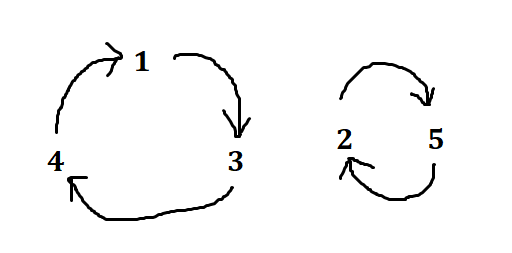
\includegraphics[scale=0.7]{assets/permutation_134_25.png}
\end{center}
This can be written in \textbf{cycle notation}:
\[p = (1 3 4)(2 5)\]
The first cycle $(1 3 4)$ is a 3-cycle and the second cycle $(2 5)$ is a 2-cycle. This brings us to our next definition: 
\begin{definition}{Transposition}{}
    A 2-cycle is also known as a \textbf{transposition}. More precisely, a transposition is a permutation that swaps two elements and fixes the rest.
\end{definition}

Now, permutations do have inverses For example, the inverse of $p$ is $p^{-1} = (1 4 3) (5 2) = (1 4 3) (2 5)$. Drawing it out yields: 
\begin{center}
    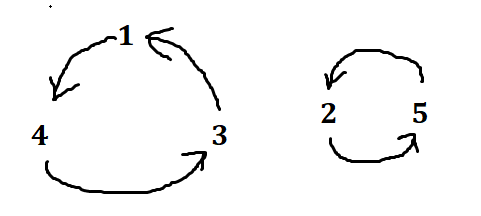
\includegraphics[scale=0.7]{assets/permutation_134_25_i.png}
\end{center}
Essentially, all we did was change what directions the arrow pointed to.

\subsection{Writing Cycles and Fixed Elements}
Suppose we had the permutation $p = (2143)(5)$. We note that all this is saying is: 
\begin{itemize}
    \item 2 goes to 1. 
    \item 1 goes to 4. 
    \item 4 goes to 3. 
    \item 3 goes to 2.
\end{itemize}
We can write the first cycle like so: 
\[(2143) = (3214) = (4321) = (1432)\]
These all say the same thing. So, to be consistent, we write cycles out like so: 
\begin{enumerate}
    \item Start at \code{1}, trace it out as it cycles. 
    \item Find the smallest unused index in the next cycle. Repeat. 
    \item Omit cycles of length 1. If all cycles are of length 1, then it is the identity permutation and so we can write $(1)$. 
\end{enumerate}
In this permutation example, we do have a cycle of length 1: that would be $(5)$. All \emph{this} is saying is that 5 goes to 5. Usually, we omit it since it doesn't tell us anything. Then, it follows that \emph{if a number isn't in the cycle representation of a permutation}, then that number is fixed. For example, $q = (134)$ means that: 
\begin{itemize}
    \item 1 goes to 3. 
    \item 3 goes to 4. 
    \item 4 goes to 1. 
    \item 2 is fixed. 
\end{itemize}

\subsection{Symmetric Groups}
Now, we can introduce the notion of a symmetric group. 
\begin{definition}{Symmetric Group}{}
    For some $n \in \Z^+$, a \textbf{symmetric group} is the group of all permutations of the indices $\{1, 2, \dots, n\}$ and is denoted by $S_n$. This is denoted by $S_n$ and has order $n!$. 
\end{definition}
\textbf{Remark:} While the order of a symmetric group of $n$ elements is $n!$, the order of a \emph{permutation} is the \underline{least common multiple} of the lengths of the \emph{disjoint} cycles. For example, the order of $(12)(3456)(78)$ is $\lcm(2, 4) = 4$. 

\bigskip 

A common symmetric group is $S_3 = \{(1), (12), (13), (23), (123), (132)\}$. 

\subsection{Decomposition of Permutations}
A permutation $\sigma$ can be decomposed into non-disjoint transpositions like so: 
\[\sigma = (a_1, a_2, \dots, a_{n - 1}, a_n) = (a_1, a_2)(a_2, a_3) \dots (a_{n - 2}, a_{n - 1})(a_{n - 1}, a_n) \in S_n\]
For instance, suppose $\sigma = (123)(4567)$. Then, we can decompose this permutation like so: 
\[(123)(4567) = \underbrace{(12)(23)}_{(123)}\overbrace{(45)(56)(67)}^{(4567)}\]

\subsection{Sign of a Permutation}
We can define the sign of a permutation by the following function: 
\[\text{sgn}: S_n \mapsto \{\pm1\}\]
A permutation is said to be \textbf{even} if its sign is 1. Conversely, a permutation is odd if its sign is -1. 

\subsubsection{Sign of a Cycle}
The sign of a cycle is simply $(-1)^{\ell - 1}$, where $\ell$ is the length of the given cycle. For example, consider the permutation $\sigma = (12345) \in S_5$, which consists of an individual cycle. $\sigma$ has a length of 5, so its sign is:
\[(-1)^{5 - 1} = (-1)^4 = 1\] 

\subsubsection{Sign of Permutations}
Of course, we can represent permutations with multiple cycles. So, we can find the sign of any permutation by multiplying the sign of each cycle together. For instance, consider the permutation $\sigma = (123)(4567) \in S_7$. Then: 
\begin{equation*}
    \begin{aligned}
        \text{sgn}(\sigma) &= \text{sgn}((123)(4567)) \\ 
            &= \text{sgn}((123)) \text{sgn}((4567)) \\ 
            &= (-1)^{3 - 1} (-1)^{4 - 1} \\ 
            &= (-1)^2 (-1)^3 \\ 
            &= -1
    \end{aligned}
\end{equation*}
This can be extended to three, four, or more cycles. For $n$ cycles, we can generalize this formula like so: 
\begin{equation*}
    \begin{aligned}
        \text{sgn}(\sigma) &= \text{sgn}(\text{Cycle 1}) \cdot \text{sgn}(\text{Cycle 2}) \cdot \ldots \cdot \text{sgn}(\text{Cycle n}) \\
            &= (-1)^{\text{(Length of Cycle 1)} - 1} \cdot (-1)^{\text{(Length of Cycle 2)} - 1} \cdot \ldots \cdot (-1)^{\text{(Length of Cycle n)} - 1}
    \end{aligned}
\end{equation*}
\textbf{Remark:} In this example, we made use of the fact that $\text{sgn}$ is a \emph{homomorphism}; this will be discussed in the next major section. 

\subsubsection{Sign of Transpositions}
Recall that we can also decompose permutations into non-disjoint transpositions. The number of transpositions also defines the sign. In particular: 
\[\text{sgn}(\sigma) = (-1)^{\text{Number of Transpositions}}\]
Take our example $\sigma = (123)(4567) \in S_7$. We know that $\sigma$ can be decomposed like so: 
\[\sigma = (123)(4567) = (12)(23)(45)(56)(67) \in S_7\]
So, $\sigma$ can be represented by \textbf{5} transpositions. Therefore:
\[(-1)^{5} = -1\]
So, actually, a better definition of even and odd permutations is as follows: 
\begin{itemize}
    \item A permutation is \emph{even} if it can be written as a product of an even number of transpositions. 
    \item A permutation is \emph{odd} if it can be written as a product of an odd number of transpositions.
\end{itemize}

\subsection{Alternating Group}
We now talk about alternating groups, a subgroup of the symmetric group. 
\begin{definition}{Alternating Group}
    The \textbf{alternating group} $A_n$ is the group of \emph{even} permutations. 
\end{definition}
We now show that this is a subgroup of the symmetric group. 
\begin{mdframed}
    \begin{proof}
        To show that $A_n$ is a subgroup, we need to show that all properties of a subgroup are satisifed. First, We know that $(1)$, the identity permutation, is an even permutation, so $(1) \in A_n$. Next, if $\tau$ and $\sigma$ are even, then it follows that $\tau^{-1}$ is even (decompose $\tau$ into transpositions and write the product backwards). Therefore, $\sigma\tau^{-1}$ is even and so $\sigma\tau^{-1} \in A_n$. 
    \end{proof}
\end{mdframed}

For example, we know that $S_3 = \{(1), (12), (13), (23), (123), (132)\}$. So: 
\[A_3 = \{(1), (123), (132)\}\]
The alternating group has order $\frac{n!}{2}$, where $n$ is the number of elements.








\newpage 
\section{Homomorphisms}
We will now discuss homomorphisms, which is one of the more important concepts to know.  

\subsection{Motivating Examples}
We begin the discussion of homomorphisms with two motivating examples.

\subsubsection{Motivating Example 1: Modulo Addition}
Let's suppose we are given two groups: 
\begin{itemize}
    \item \underline{Group 1:} $(\Z, +)$. 
    \item \underline{Group 2:} $(\Z / \Z 2, +)$.
\end{itemize}
These two groups may look completely unrelated at first. However, we note the following behaviors between the two groups:

\begin{center}
    \begin{tabular}{c|c}
        Operation in $(\Z, +)$ & Operation in $(\Z / \Z 2, +)$ \\ 
        \hline 
        Even + Even = Even. & $0 + 0 \equiv 0 \mod{2}$. \\ 
        Even + Odd = Odd. & $0 + 1 \equiv 1 \mod{2}$. \\ 
        Odd + Even = Odd. & $1 + 0 \equiv 1 \mod{2}$. \\ 
        Odd + Odd = Even. & $1 + 1 \equiv 0 \mod{2}$.
    \end{tabular}
\end{center}

Something to note here is that we can easily map:
\begin{itemize}
    \item \code{Even} (in first group) $\mapsto$ \code{0} (in second group).
    \item \code{Odd} (in first group) $\mapsto$ \code{1} (in second group).
\end{itemize}
This mapping can be represented like so: 
\[\varphi: \Z \mapsto \Z / \Z 2\]
Where: 
\begin{itemize}
    \item If $x \in \Z$ is even, map it to $0 \in \Z / \Z 2$. 
    \item If $x \in \Z$ is odd, map it to $1 \in \Z / \Z 2$. 
\end{itemize}
Although these two groups appear to be completely unrelated, they are, in fact, related. 

\subsubsection{Example 2: Generalized Tables}
Suppose we have two groups $(G, *)$ and $(G', \cdot)$. They can be infinite, finite, commutative, non-commutative, etc. Suppose we have two elements $x, y \in G$. Then, we also know that $x * y \in G$ (closure). 

\bigskip 

Let's suppose we can represent the operations of the above group using a table, like so: 
\begin{itemize}
    \item \underline{Group 1:} $(G, *)$. Since we know that $x$, $y$, and $x * y \in G$, they'll appear in this table. 
    \begin{center}
        \begin{tabular}{|c|c c c|c|c|}
            \hline 
            $*$     & \dots & \dots & \dots & $y$     & \dots \\ 
            \hline 
            \vdots  &       &       &       &         &       \\ 
            \vdots  &       &       &       &         &       \\ 
            \hline 
            $x$     &       &       &       & $x * y$ &       \\ 
            \hline 
            \vdots  &       &       &       &         &       \\ 
            \vdots  &       &       &       &         &       \\ 
            \hline 
        \end{tabular}
    \end{center}

    \item \underline{Group 2:} $(G', \cdot)$. In order for these groups to have similar group behavior, $x$, $y$, and $x * y$ in $G$ must correspond to the elements in $G'$. This can be represented by a function: 
    \[\varphi: G \mapsto G'\]
    We want this function to send a specific part of the table for $G$ to a similar part of the table for $G'$. In this sense, we can say that the place where $x \in G$ is (in the above table) can be mapped to a similar place in the below table for $G'$; the same idea applies to $y \in G$ and $x * y \in G$.  
    \begin{center}
        \begin{tabular}{|c|c c c|c|c c|}
            \hline 
            $\cdot$   & \dots & \dots & \dots & $\varphi(y)$      & \dots & \dots \\ 
            \hline 
            \vdots    &       &       &       &                &       &        \\ 
            \vdots    &       &       &       &                &       &        \\ 
            \hline 
            $\varphi(x)$ &       &       &       & $\varphi(x * y)$  &       &        \\ 
            \hline 
            \vdots    &       &       &       &                &       &        \\ 
            \vdots    &       &       &       &                &       &        \\ 
            \vdots    &       &       &       &                &       &        \\ 
            \hline 
        \end{tabular}
    \end{center}
    Here, we got $\varphi(x)$, $\varphi(y)$, and $\varphi(x * y)$ from the function mapping. The function mapping essentially mapped $x$, $y$, and $x * y$ to ``similar'' locations in the $G'$ table. 

    \bigskip 

    An observation to note here is that the square where $\varphi(x * y)$ is at (in the table above) must also contain $\varphi(x) \cdot \varphi(y)$. 
\end{itemize}




\subsection{Definition of Homomorphism}
\begin{definition}{Homomorphism}{}
    Let $(G, *)$ and $(G', \cdot)$ be two different groups. A \textbf{homomorphism} (also known as a \emph{group homomorphism}) from $G$ to $G'$ is a function: 
    \[\varphi: G \mapsto G'\]
    Such that for all $a, b \in G$, $\varphi(a * b) = \varphi(a) \cdot \varphi(b)$. 
\end{definition}
\textbf{Remark:} Here, we say that: 
\[\underbrace{\varphi(a * b)}_{\text{Binary operation in } G} = \overbrace{\varphi(a) \cdot \varphi(b)}^{\text{Binary operation in } G'}\]

\subsection{Pictorial Interpretation}
A visualization of this process is shown below: 
\begin{center}
    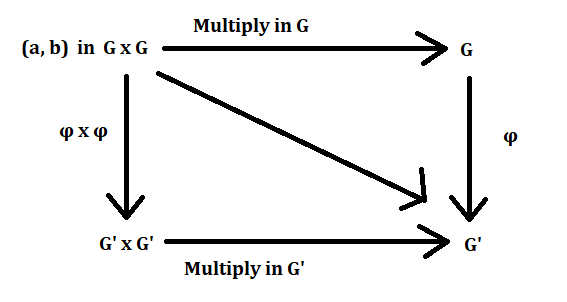
\includegraphics[scale=0.7]{assets/homo_diagram.png}
\end{center}
This is known as a \emph{commutative diagram}.

\subsection{Examples of Homomorphisms}
We will now discuss some simple example of homomorphisms. 

\subsubsection{Example: Integers}
Consider the following function: 
\[c_n: (\Z, +) \mapsto (\Z / \Z n, +)\]
Defined by: 
\[c_{n}(a) = [a]_n\]
We can say that $c_n$ is a group homomorphism since for all $a, b \in \Z$: 
\[c_{n}(a + b) = [a + b]_n = [a]_n + [b]_n = c_{n}(a) + c_{n}(b)\]

\subsubsection{Example: Function Negation}
Consider the following function: 
\[f: (\Z, +) \mapsto (\Z, +)\]
Defined by: 
\[f(x) = -x\]
Then, we say that $f$ is a group homomorphism since for all $x, y \in \Z$: 
\[f(x + y) = -(x + y) = (-x) + (-y) = f(x) + f(y)\]

\subsubsection{Example: Exponential Map}
Consider the following function: 
\[\varphi: (\R, +) \mapsto (\R - \{0\}, \times)\]
Defined by: 
\[\varphi(x) = e^x\]
Then, $\varphi$ is a group homomorphism since for all $x, y \in \R$: 
\[\varphi(x + y) = e^{x + y} = e^x \times e^y = \varphi(x) \times \varphi(y)\]


\subsubsection{Example: Generalized Exponential Map}
Suppose $(G, *)$ is a group and $g \in G$. Then, we can consider the following function: 
\[f: (\Z, +) \mapsto (G, *)\]
Defined by: 
\[f(n) = g^n\]
We know that this is a group homomorphism because for every $m, n \in Z$:
\[f(m + n) = g^{m + n} = g^m * g^n = f(m) * f(n)\]

\subsubsection{Example: Logarithmic Map}
Consider the following logarithmic function: 
\[\ln: (\R_{> 0}, \times) \mapsto (\R, +)\]
We know that this is a group homomorphism since for all $x, y \in \R_{ > 0}$: 
\[\ln(x \times y) = \ln(x) + \ln(y)\]

\subsubsection{Example: Complex Numbers}
Consider the following function: 
\[N: (\C - \{0\}, \times) \mapsto (\R_{> 0}, \times)\]
Defined by: 
\[N(z) = |z|\]
This is a group homomorphism because for every $z \in \C - \{0\}$ and $|z| \in \R_{> 0}$:
\[|z_1 \times z_2| = |z_1| \times |z_2|\]

\subsubsection{Example: Matrices}
Define $(GL_{n}(\R), \cdot)$ be the set of invertible $n \times n$ real matrices under matrix multiplication.\footnote{From linear algebra, we know that matrix multiplication is associative, the product of two invertible $n \times n$ is invertible, and for every $a \in GL_{n}(\R)$, $a \cdot I_n = I_n \cdot a = a$ where $I_n$ is the identity matrix.} Consider the function: 
\[\theta: GL_{n}(\R) \mapsto GL_{n}(\R)\]
Defined by\footnote{If $x$ is a matrix, then $x^T$ is the transpose of said matrix.}: 
\[\theta(x) = (x^T)^{-1}\]
We know that $\theta$ is a group homomorphism because: 
\[\theta(x \cdot y) = ((x \cdot y)^T)^{-1} = (y^T \cdot x^T)^{-1} = (x^T)^{-1} \cdot (y^T)^{-1} = \theta(x) \cdot \theta(y)\]

\subsection{Properties of Homomorphisms}
\begin{mdframed}
    \begin{proposition}
        Let $\varphi: G \mapsto G'$ be a group homomorphism. 
        \begin{enumerate}[(a)]
            \item $\varphi$ maps the identity to the identity: $\varphi(\id_G) = \id_{G'}$. 
            \item $\varphi$ maps inverses to inverses; in other words, for every $a \in G$, $\varphi(a^{-1}) = \varphi(a)^{-1}$ where $a^{-1}$ is the inverse of $a$ in $G$ and $\varphi(a)^{-1}$ is the inverse of $\varphi(a)$ in $G'$. This can also be written as: 
            \[\id_G = \varphi(a) \varphi(a^{-1})\]
            \item If $a_1, \dots, a_k$ are elements of $G$, then $\varphi(a_1, \dots, a_k) = \varphi(a_1) \dots \varphi(a_k)$. 
        \end{enumerate}
    \end{proposition}
\end{mdframed}

The proof is as follows: 
\begin{mdframed}
    \begin{proof}
        We need to show that all three properties hold. 
        \begin{enumerate}[(a)]
            \item We note that since $\id_G$ is the identity element of $G$, it follows that $\id_G * \id_G = \id_G$. Because $\varphi$ is a group homomorphism, it follows that: 
            \[\boxed{\varphi(\id_G * \id_G)} = \varphi(\id_G) * \varphi(\id_G)\]
            Since $\id_G * \id_G = \id_G$, it follows that $\varphi(\id_G * \id_G) = \varphi(\id_G)$, so: 
            \[\varphi(\id_G) * \varphi(\id_G) = \boxed{\varphi(\id_G)}\]
            Thus: 
            \[\varphi(\id_G) * \varphi(\id_G) = \varphi(\id_G) * \id_{G'}\]
            Canceling the first element in each side, we now have: 
            \[\varphi(\id_G) = \id_{G'}\]

            \item For every $a \in G$, we know that $a * a^{-1} = \id_G$. Applying $\varphi$ to both sides, we have that: 
            \[\varphi(a * a^{-1}) = \varphi(\id_G)\]
            By the first part and the fact that $\varphi$ is a group homomorphism, we deduce that: 
            \[\varphi(a) * \varphi(a^{-1}) = \id_{G'}\]
            Multiplying both sides by the inverse $\varphi(a)^{-1}$ of $\varphi(a)$ in $G'$, we obtain: 
            \[\varphi(a)^{-1} * \varphi(a) * \varphi(a^{-1}) = \varphi(a)^{-1} * \id_H\]
            And so:
            \[\varphi(a^{-1}) = \varphi(a)^{-1}\]

            \item We can simply make use of induction from the definition. \qedhere
        \end{enumerate}
    \end{proof}
\end{mdframed}


\subsection{Image}
\begin{definition}{Image}{}
    The \textbf{image} of a general homomorphism $\varphi: G \mapsto G'$ is simply the image of $\varphi$ as a map of sets: 
    \[\im(\varphi) = \{x \in G' \mid x = \varphi(a) \text{ for some } a \in G\}\]
    More simply: 
    \[\im(\varphi) = \{\varphi(g) \mid g \in G\}\]
\end{definition}
The image of $\varphi$ is a subgroup of $G'$. Say $a, b \in G'$ are in the image; that is, $\exists x, y \in G$ such that $\varphi(x) = a$, $\varphi(y) = b$. Then: 
\[\varphi(xy) = ab\]
This implies that the image has closure. The image has the identity (consider the second property in the propositions). Finally, the image has the inverse since $\varphi(x^{-1}) = a^{-1}$. 

\subsection{Kernal}
\begin{definition}{Kernal}{}
    The \textbf{kernal} of a general homomorphism $\varphi: G \mapsto G'$ is the set of elements of $G$ that are mapped to the identity in $G'$: 
    \[\ker(\varphi) = \{a \in G \mid \varphi(a) = \id_{G'}\}\]
\end{definition}
Here, the kernal of $\varphi$ is a subgroup of $G$. 


\subsubsection{Example: Matrices}
For example, we have that $\varphi: \det GL_n (\R) \mapsto (\R - \{0\}, \times)$, which means that: 
\[\ker(a) = SL_n\]
Where $SL_n$ is the special linear group of $n \times n$ matrices. 

\subsection{Conjugation}
For a fixed $g \in G$ where the binary operation is $*$, the function: 
\[\varphi: G \mapsto G\]
Defined by: 
\[\varphi(a) = g^{-1} * a * g\]
Is a homomorphism. In particular, we call this the conjugate. This is a homomorphism because: 
\begin{equation*}
    \begin{aligned}
        \varphi(a * b) &= \varphi(a) * \varphi(b) \\ 
            &= (g^{-1} * a * g) * (g^{-1} * b * g) \\ 
            &= g^{-1} * a * (g * g^{-1}) * b * g \\ 
            &= g^{-1} * a * b * g
    \end{aligned}
\end{equation*}
We will discuss this more in-depth later on. 





\newpage 
\section{Isomorphisms}
We now discuss isomorphisms, a special type of homomorphisms.

\subsection{Motivating Example}
Before we talk about isomorphisms, let's first talk about two motivating examples. 

\subsubsection{Motivating Example 1: Tables}
Let's suppose we are given two groups.
\begin{itemize}
    \item \underline{Group 1:} $(\Z / \Z 4, +)$. 
    \item \underline{Group 2:} $(\{1, -1, i, -i\}, \times)$
\end{itemize}
At first, these groups don't look at all related to each other. They even have completely different operations. However, they are structurally similar. 

\bigskip 

Consider the table that represents group 1:
\begin{center}
    \begin{tabular}{c|c c c c}
        $+$     & 0 & 1 & 2 & 3 \\ 
        \hline 
        0       & 0 & 1 & 2 & 3 \\
        1       & 1 & 2 & 3 & 0 \\ 
        2       & 2 & 3 & 0 & 1 \\ 
        3       & 3 & 0 & 1 & 2
    \end{tabular}
\end{center}
Now, consider the table that represents group 2: 
\begin{center}
    \begin{tabular}{c|c c c c}
        $\times$ & 1 & $i$ & $-1$ & $-i$ \\ 
        \hline 
        1        & 1 & $i$ & $-1$ & $-i$ \\ 
        $i$      & $i$ & $-1$ & $-i$ & 1 \\ 
        $-1$     & $-1$ & $-i$ & 1 & $i$ \\ 
        $-i$     & $-i$ & 1 & $i$ & $-1$
    \end{tabular}
\end{center}
One thing that should be clear (after some observation) is how the elements in both tables correspond with each other. Consider the same tables from above, now highlighted: 
\begin{center}
    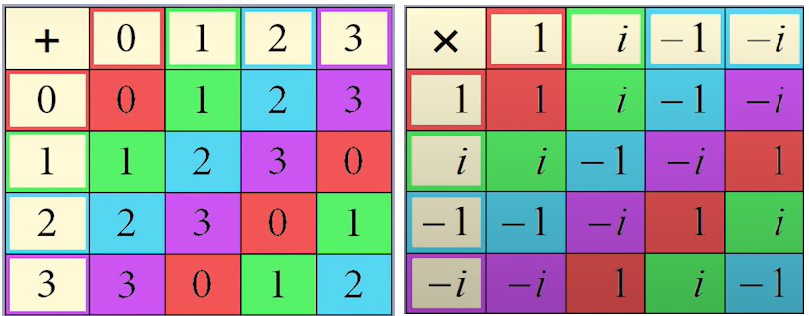
\includegraphics[scale=0.5]{assets/homo_ex.png}
\end{center}
Both tables exhibit the same patterns. They're essentially identical groups; they just use different elements and different operations. For instance, in both tables, if we combined a green element with a blue element, we get a purple element. If we combined a blue element with a blue element, we get a red element. In other words, any statement about one table can be said for the other. 

\bigskip 

We say that these two groups are \emph{isomorphic} (equal form). 

\subsubsection{Motivating Example 2: Addition Table}
Consider the following addition table of $(\Z / \Z_3, +)$.
\begin{center}
    \begin{tabular}{c|c c c}
        $+$     & $[0]_3$ & $[1]_3$ & $[2]_3$ \\ 
        \hline 
        $[0]_3$ & $[0]_3$ & $[1]_3$ & $[2]_3$ \\
        $[1]_3$ & $[1]_3$ & $[2]_3$ & $[0]_3$ \\
        $[2]_3$ & $[2]_3$ & $[0]_3$ & $[1]_3$ 
    \end{tabular}
\end{center}
Now, consider the Roman numbers: 
\begin{center}
    \begin{tabular}{c|c c c}
        $+$     & 0 & I & II \\ 
        \hline 
        0       & 0 & I & II \\ 
        I       & I & II & 0 \\ 
        II      & II & 0 & 1
    \end{tabular}
\end{center}
It's clear that both of these are the same groups, only written with different symbols. We only need a \emph{translator} to tell us which one is which. What is a translator (in the context of a group)? It should be a \emph{bijection} which preserves the operation table. Notice that preserving the operation table simply means that it should be a group homomorphism. This brings us to the definition of group isomorphism. 


\subsection{Definition of Isomorphism}
\begin{definition}{Isomorphism}{}
    An \textbf{isomorphism} of two groups $(G, *)$ and $(G', \cdot)$ is a \underline{bijective} \emph{homomorphism}: 
    \[\varphi: G \mapsto G'\]
    If there is a isomorphism $\varphi: G \mapsto G'$, we say that $G$ is isomorphic to $G'$ and write $G \cong G'$. 
\end{definition}
\textbf{Remark:} To say that two groups are isomorphic is to say that they are the same as \emph{groups}. The elements of the two groups, and the associated group operations, may be different; however, both groups have the same exact structures.

\subsection{Inverse of Isomorphism}
\begin{lemma}{}{}
    A homomorphism $\varphi: G \mapsto G'$ is an isomorphism if and only if it is invertible. In this case, $\varphi^{-1}$ is also a homomorphism, hence an isomorphism.
\end{lemma}
\begin{mdframed}
    \begin{proof}
        The first statement here is trivial, since a map of sets is bijective if and only if it has an inverse. Now, suppose $\varphi: G \mapsto G'$ is an isomorphism. Then, we need to show that $\varphi^{-1}: G' \mapsto G$ is a homomorphism. To make things explicit, suppose $G$ has the binary operation $*$ and $G'$ has the binary operation $\cdot$. Let $x, y \in G'$; then, we need to show that: 
        \[\varphi^{-1}(x \cdot y) = \varphi^{-1}(x) * \varphi^{-1}(y)\]
        Since $\varphi: G \mapsto G'$ is surjective, there exists $a, b \in G$ such that $\varphi(a) = x$ and $\varphi(b) = y$. Then: 
        \[\varphi^{-1}(x \cdot y) = \varphi^{-1}(\varphi(a) \cdot \varphi(b)) = \varphi^{-1}(\varphi(a * b)) = a * b = \varphi^{-1}(x) * \varphi^{-1}(y)\]
        Therefore, $\varphi^{-1}$ is a homomorphism. Since $\varphi^{-1}$ is invertible, its inverse being $\varphi$, it is an isomorphism by the first part of the lemma. 
    \end{proof}
\end{mdframed}

\subsection{Pictorial Interpretation}
A pictorial interpretation can be seen as follows: 
\begin{center}
    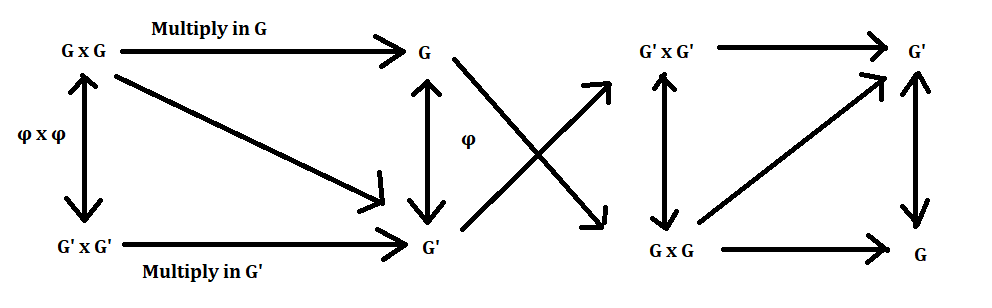
\includegraphics[scale=0.6]{assets/iso_diagram.png}
\end{center}

\subsection{Properties of Isomorphisms}
We say that $G$ and $G'$ are isomorphism if there exists some isomorphism between them. Any \emph{purely structural} property of a group is isomorphism-stable in the sense that if $G$ and $G'$ are isomorphic and $G$ has a property, then $G'$ does as well. 

\bigskip 

Some examples of structural properties include: 
\begin{itemize}
    \item Being finite. 
    \item Having order $n$ for any $n$. 
    \item Being cyclic. 
    \item Being abelian/commutative. 
    \item Number of elements of a given order. 
\end{itemize}

\textbf{Remarks:}
\begin{itemize}
    \item $\Z / \Z 6$ is not isomorphic to $S_3$ because $\Z / \Z 6$ is commutative but $S_3$ is not. 
    \item Any two cyclic groups of the same order are isomorphic. 
\end{itemize} 

\subsubsection{Abelian Structure}
\begin{mdframed}
    \begin{proposition}
        Suppose $G$ and $G'$ are isomorphic groups. If $G$ is abelian, then so is $G'$. 
    \end{proposition}
\end{mdframed}

\begin{mdframed}
    \begin{proof}
        We once again take $G$ to have binary operation $*$ and $G'$ to have binary operation $\cdot$. Take $x, y \in G'$. Since $G$ and $G'$ are isomorphic, then let $\varphi(a) = x$ and $\varphi(b) = y$ where $a, b \in G$. Then: 
        \begin{equation*}
            \begin{aligned}
                x \cdot y &= \varphi(a) \cdot \varphi(b) \\ 
                    &= \varphi(a * b) && \varphi \text{ is a homomorphism.} \\ 
                    &= \varphi(b * a) && G \text{ is abelian (commutative).} \\ 
                    &= \varphi(b) \cdot \varphi(a) && \varphi \text{ is a homomorphism.} \\ 
                    &= y \cdot x
            \end{aligned}
        \end{equation*}  
        Therefore, $G'$ is abelian. 
    \end{proof}
\end{mdframed}

\subsubsection{Order Structure}
\begin{mdframed}
    \begin{proposition}
        Suppose $G$ and $G'$ are isomorphic groups. If $G$ has a subgroup $K$ of order $n$, so does $G'$.
    \end{proposition}
\end{mdframed}

\begin{mdframed}
    \begin{proof}
        Since $K$ is a subgroup of $G$ and $|K| = n$, then $\varphi(K)$ is a subgroup of $G'$. Since $\varphi$ maps $K$ bijectively onto $\varphi(K)$, it follows that $|\varphi(K)| = n$. 
    \end{proof}
\end{mdframed}


\subsubsection{Examples of Non-Cyclic Isomorphisms}
The following examples are isomorphic to each other: 
\begin{itemize}
    \item The Klein Four Group: 
    \begin{center}
        \begin{tabular}{c|c c c c}
                & 1 & $a$ & $b$ & $c$ \\ 
            \hline 
            1   & 1 & $a$ & $b$ & $c$ \\ 
            $a$ & $a$ & 1 & $c$ & $b$ \\ 
            $b$ & $b$ & $c$ & 1 & $a$ \\ 
            $c$ & $c$ & $b$ & $a$ & 1
        \end{tabular}
    \end{center}

    \item $H \subseteq S_4$: 
    \[\left\{1, (12)(34), (13)(24), (14)(23)\right\}\]

    \item $(\Z / \Z 8 - \{0\}, \times)$
    \[\{1 \Mod{8}, 3 \Mod{8}, 5 \Mod{8}, 7 \Mod{8}\}\]
\end{itemize}
Even though these examples are completely different, they are isomorphic (they are very similar in \emph{structure}). 










\newpage 
\section{Equivalence Relations}
We will briefly talk about equivalence relations, which are particularly important for near-future topics like cosets.

\bigskip 

\textbf{Note:} A lot of the notes here was taken from Professor Golsefidy's Math 103A notes. 

\subsection{Definition}
Let $S$ be a non-empty set. Then, a \textbf{relation} over $S$ is a subset $R$ of $S \times S$. If $(x, y) \in R$, we say that $x$ is $R$-related to $y$ and write $x R y$. 

\bigskip 

So, for these relations, we should think about inequalities equalities, or congruences between integers. 

\bigskip 

Suppose $R$ is a relation over $S$. Then:
\begin{itemize}
    \item $R$ is called \textbf{reflexive} if $\forall x \in S$, $x R x$. That is, every $x \in S$ is related to itself. 
    \item $R$ is called \textbf{symmetric} if $\forall x, y \in S$, $x R y \implies y R x$. In other words, if $x$ is related to $y$, is $y$ related to $x$? 
    \item $R$ is called \textbf{transitive} if $\forall x, y, z \in S$, $x R y$ and $y R z$ implies that $x R z$. 
\end{itemize}

\begin{definition}{Equivalence Relation}{equivRel}
    An \textbf{equivalence relation} on a set $S$ is a relation that holds between certain pairs of elements of $S$. We may write it as $a \sim b$ and speak of it as \emph{equivalence} of $a$ and $b$ (or simply, $a$ is equivalent to $b$). An equivalence relation is required to be: 
    \begin{itemize}
        \item \underline{Reflexive:} For all $a$, $a \sim a$. 
        \item \underline{Symmetric:} $\forall a, b \in S$, if $a \sim b$, then $b \sim a$. 
        \item \underline{Transitive:} $\forall a, b, c \in S$, if $a \sim b$ and $b \sim c$, then $a \sim c$. 
    \end{itemize}
\end{definition}

\textbf{Remarks:}
\begin{itemize}
    \item An equivalence relation is essentially an equality with respect to a certain measurement. In life, we often measure things or people with respect to properties (for example, scores or ratings). So, when we want to compare things, we pick a certain property and then, \emph{from that point of view}, determine whether these things are equal. In this regard, equivalence relations are exactly equalities. 
    \item Another way we can think of an equivalence relation is through a function: 
    \[S \times S \mapsto \{\text{true}, \text{false}\}\]
\end{itemize} 

\subsubsection{Example: Relations}
Suppose $X$ and $Y$ are two non-empty sets and $f: X \mapsto Y$ is a function. Let $\sim$ be the following relation over $X$:
\[\forall x_1, x_2 \in X \quad x_1 \sim x_2 \iff f(x_1) = f(x_2)\]
Then, $\sim$ is an equivalence relation\footnote{Another way of interpreting this statement is as follows: $x_1$ is in relation to $x_2$ precisely when $f(x_1) = f(x_2)$. The claim here, then, is that this is an equivalence relation.}.

\begin{mdframed}
    \begin{proof}
        We determine if an relation is an equivalence relation if it satisfies the three properties mentioned above.
        \begin{itemize}
            \item \underline{Reflexivity:}
            \[\forall x \in X, f(x) = f(x) \implies x \sim x\]
    
            \item \underline{Symmetric:}
            \[x_1 \sim x_2 \implies f(x_1) = f(x_2) \implies f(x_2) = f(x_1) \implies x_2 \sim x_1\]
    
            \item \underline{Transitive:}
            We know that:
            \[\forall x_1, x_2 \in X \qquad x_1 \sim x_2 \implies f(x_1) = f(x_2)\]
            We also know that:
            \[\forall x_2, x_3 \in X \qquad x_2 \sim x_3 \implies f(x_2) = f(x_3)\]
            It follows that if $f(x_1) = f(x_2)$ and $f(x_2) = f(x_3)$, then $f(x_1) = f(x_3)$ and thus, $x_1 = x_3$. Namely, $x_1 \sim x_2$ and $x_2 \sim x_3$, then $x_1 \sim x_3$. 
        \end{itemize}
        It follows that this is an equivalence relation. 
    \end{proof}
\end{mdframed}

\subsection{Equivalence Relation Partitions}
Recall that $P$ is called a \textbf{partition} of a non-empty set $X$ if:
\begin{itemize}
    \item \underline{Subsets:} $P$ consists of non-empty subsets of $X$. 
    \item \underline{Disjointness:} $A, B \in P$ and $A \neq B \implies A \cap B = \emptyset$. In other words, the subsets are disjoint. 
    \item \underline{Covering:} $\forall x \in X$, $\exists A \in P$ such that $x \in A$. In other words, every element in $X$ will be in one of the subsets. Alternatively, $\bigcup_{A \in P} A = X$. 
\end{itemize}

\textbf{Remark:}
\begin{itemize}
    \item As mentioned, $P$ is a set of sets. For instance, if we have $X = \{1, 2, 3\}$, one possible $P$ is $P = \{\{1\}, \{2, 3\}\}$.
    \item Below is a visual diagram of what a partition may look like.
\end{itemize}
\begin{center}
    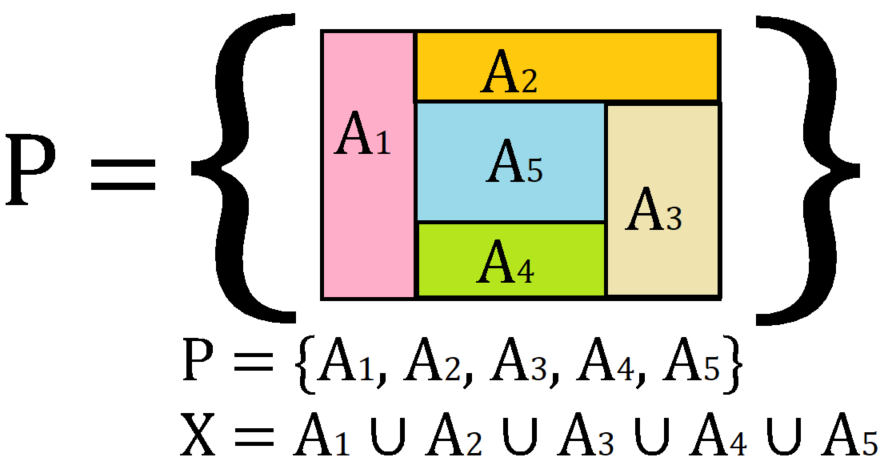
\includegraphics[scale=0.4]{assets/partition.PNG}
\end{center}

Suppose $P$ is a partition of $X$. Then, we can get a classification function from $X$ to $P$:
\[X \mapsto P\]
\[x \mapsto [x]_P\]
Here, $[x]_P$ is the unique element of $P$ which contains $x$. In other words, if we refer to the above diagram, we can think of $[x]_P$, a set, as one of the sets $A_1$, $A_2$, $A_3$, $A_4$, or $A_5$ which contains $x$. So, we can think of this function as saying that every $x \in X$ belongs to one of the sets $[x]_P$. 

\bigskip 

Notice that, because of the \textbf{covering} condition, $x$ is contained in some element of $P$; additionally, because of the \textbf{disjointness} condition, $x$ is in an unique element of $P$ (i.e. it is in \underline{one} of the sets which is in $P$). So, it follows that the function is well-defined. 

\bigskip 

By the previous example, $x \sim_P y \iff [x]_P = [y]_P$ is an equivalence relation. So, we obtain the following lemma. 
\begin{lemma}{}{}
    Suppose $P$ is a partition of a non-empty set $X$. For $x, y \in X$, $x \sim y$ if $x$ and $y$ are in the same element of $P$. Then, $\sim$ is an equivalence relation.
\end{lemma}
\textbf{Remark:} Essentially, what this lemma is saying is that if $x \sim y$, then both $x$ and $y$ are in the same set which is in $P$. In other words, if we refer to the above diagram again, we can think of this situation as saying that both $x$ and $y$ are in \underline{one} of $A_1$, $A_2$, $A_3$, $A_4$, or $A_5$. The diagram below complements the proof.

\begin{center}
    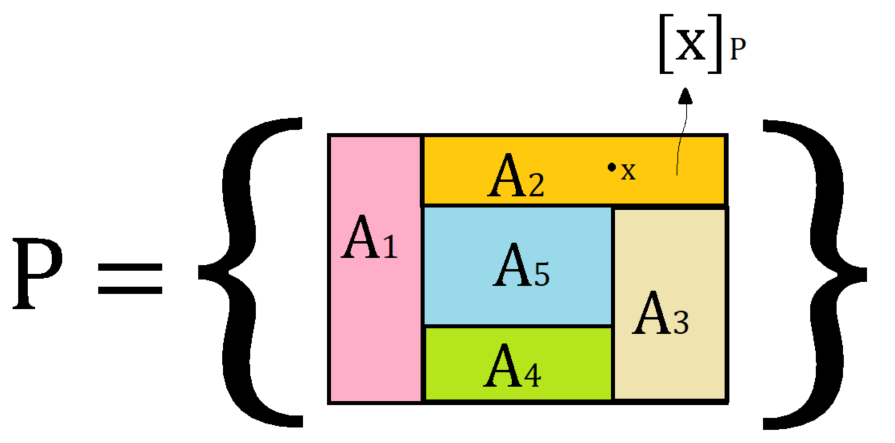
\includegraphics[scale=0.30]{assets/partition_x.PNG}
\end{center}

\begin{mdframed}
    \begin{proof}
        For $x \in X$, let $[x]_P$ to be the unique element of $P$ which contains $x$. So, $x \mapsto [x]_P$ is a function from $X \mapsto P$. By the previous example, $x \sim y \iff [x]_p = [y]_p$ is an equivalence relation over $X$. Notice that this means $x \sim y$ exactly when $x$ and $y$ are in the same element of $P$. 
    \end{proof}
\end{mdframed}

\subsection{Equivalence Relation Classes}
Now, suppose that $\sim$ is the equivalence relation over a non-empty set $X$, we can partition $X$ with respect to $\sim$. 

\bigskip 

For $x \in X$, we let $[x] = \{y \in X \mid y \sim x\}$ (all the elements that are $\sim$-related to $x$).\footnote{So, it's obvious that $[x] \subseteq X$.} We call $[x]$ the \textbf{equivalence class of $x$ with respect to $\sim$}. When $x \sim y$, we can say that $x$ is equivalent to $y$ with respect to $\sim$. 

\begin{mdframed}
    \begin{proposition}
        Suppose $\sim$ is an equivalence relation over a non-empty set $X$. Then, $\{[x] \mid x \in X\}$ is a partition of $X$. 
    \end{proposition}
\end{mdframed}
This proposition is essentially asking us to show the following properties: 
\begin{itemize}
    \item Covering: Every element of this set belongs to one of these equivalence classes. 
    \item Disjointness: If we pick two equivalence classes, they do not intersect.
\end{itemize}
The following lemma follows from this proposition.
\begin{lemma}{}{}
    \[x \sim y \iff [x] = [y]\]
\end{lemma}
\begin{mdframed}
    \begin{proof}
        We want to show that $[x] = [y] \implies x \sim y$. Recall that the equivalence class of $x$ ($[x]$) and the equivalence class of $y$ ($[y]$) are \emph{sets} and, in particular, we know that $[x]$ consists of all elements that are related to $x$, including $x$. Since $\sim$ is reflexive, we know that:
        \[x \sim x \implies x \in [x]\]
        But, since $[x] = [y]$, then it follows that $x \in [y] \implies x \sim y$. Thus, $[x] = [y] \implies x \sim y$. 
        
        \bigskip 
    
        To show that $x \sim y \implies [x] = [y]$, we need to show equality of sets $[x] = [y]$. This means that it is necessary and sufficient to prove $[x] \subseteq [y]$ and $[y] \subseteq [x]$.
        \begin{itemize}
            \item To prove $[x] \subseteq [y]$, we let $z \in [x]$. This means that $z \sim x$. However, since $x \sim y$, by transitivity, it follows that $y \sim z$, which implies that $z \in [y]$. Hence, $[x] \subseteq [y]$. 
            \item We note that $x \sim y \implies y \sim x$ by symmetry. Therefore, by the first bullet point, $[y] \subseteq [x]$.
        \end{itemize} 
        So, it follows that $x \sim y \implies [x] = [y]$. 
    \end{proof}
\end{mdframed}

Now that we proved the lemma, we can now prove the proposition. 
\begin{mdframed}
    \begin{proof}
        As mentioned, we need to show that the covering and disjointness properties exist in this partition.
        \begin{itemize}
            \item \underline{Covering:} $\forall x \in X$, we know that $x \sim x$ by the reflexive property (since $\sim$ is an equivalence relation). Thus, it follows that $x \in [x]$. This means that $x$ is related to $x$ and $x$ is an equivalence class of $x$, so every element in $X$ belongs to one of the equivalence classes. This implies that the $[x]$ sets are non-empty subsets and cover $X$.
            \item \underline{Disjointness:} Suppose $z \in [x] \cap [y]$ (both equivalence classes are not disjoint). We need to show that they are equal. We know that:
            \[z \in [x] \cap [y] \implies z \in [x] \implies z \sim x \implies [z] = [x]\]
            \[z \in [x] \cap [y] \implies z \in [y] \implies z \sim y \implies [z] = [y]\]
            Where the last two steps came from the lemma. Then, putting these two together, we have:
            \[[z] = [x] \text{ and } [z] = [y] \implies [x] = [y]\]
            We showed that $[x] \cap [y] \neq \emptyset \implies [x] = [y]$, the contrapositive of the disjointness property. 
        \end{itemize}
        Thus, the proof is complete. 
    \end{proof}
\end{mdframed}











\newpage 
\section{Cosets}
There aree two types of cosets: \emph{left} cosets and \emph{right} cosets. 

\subsection{Left Cosets}
\begin{definition}{Left Coset}{}
    Let $G$ be a group and $H$ be a subgroup. A \textbf{left coset} of $H$ in $G$ is a subset of $H$ of the form:  
    \[aH = \{ah \mid h \in H\}\]
    Where $a \in G$ is a fixed element and is called the \emph{representative} of the coset $aH$. 
\end{definition}
\textbf{Remark:} The subgroup $H$ is a particular left coset because $H = \id H$, where $\id$ is the identity element of $H$. 

\subsubsection{Abelian Example: Integers}
Let $G = (\Z, +)$ and $H = (\Z n, +)$. For some $a \in G$, the left coset is defined by: 
\[aH = \{\dots, a - 2n, a - n, a, a + n, a + 2n, \dots\}\]
This represents the entire residue class of $a \Mod{n}$. 

\subsubsection{Non-Abelian Example: Permutations}
Let $G = S_3 = \{(1), x, x^2, y, xy, x^2 y\}$. Define $x = (123)$ and $y = (12)$. Finally, define the subgroup:
\[H = \cyclic{y} = \{(1), y\}\] 
Then: 
\begin{center}
    \begin{tabular}{c|c}
        $\mathbf{a \in S_3}$ & $\mathbf{aH}$ \\ 
        \hline 
        $(1)$       & $(1)H = \{1, y\}$ \\ 
        $x$         & $xH = \{x, xy\}$ \\ 
        $x^2$       & $x^2 H = \{x^2, x^2 y\}$ \\ 
        $y$         & $yH = \{y, 1\} = \{1, y\} = (1)H$ \\ 
        $xy$        & $xyH = \{xy, x\} = \{x, xy\} = xH$ \\ 
        $x^2 y$     & $x^2 yH = \{x^2 y, x^2\} = \{x^2, x^2 y\} = x^2 H$
    \end{tabular}
\end{center}
So, there are three left cosets:
\[\underbrace{\{(1), y\}}_{(1)H = yH} \qquad \underbrace{\{x, xy\}}_{xH = xyH} \qquad \underbrace{\{x^2, x^2 y\}}_{x^2 H = x^2 yH}\]
Notice that the left cosets here partition $S_3$.

\subsection{Left Cosets and Partitions}
Consider the following corollary: 
\begin{corollary}{}{}
    The left cosets of $H$ in $G$ form a \underline{partition} of $G$. Equivalently, the left cosets of $H$ in $G$ form an equivalence relation: 
    \[a \sim b \text{ if } b = ah \text{ for some } h \in H\]
\end{corollary}
\begin{mdframed}
    \begin{proof}
        We'll show that the left cosets of $H$ form an equivalence relation. To do so, we show that the three properties of an equivalence relation is satisifed.  
        \begin{itemize}
            \item \underline{Reflexive:} For all $a \in G$, we know that: 
            \[a = a * \id\]
            Where $\id \in H$ is the identity element. Therefore, $a \sim a$; $a$ is in its own left coset. 
            
            \item \underline{Symmetric:} If $a \sim b$, this implies that $b = ah$ for some $h \in H$. This further implies that $a = bh^{-1}$ for $h^{-1} \in H$, which shows that $b \sim a$. 
            
            \item \underline{Transitivity:} If $a \sim b$ and $b \sim c$, then $b = ah_1$ and $c = bh_2$. Then, $c = (ah_1)h_2 = a(h_1 h_2)$ for $h_1, h_2 \in H$. By closure, it follows that $a \sim c$. 
        \end{itemize}
        So, we are done. 
    \end{proof}
\end{mdframed}

An alternative proof is as follows: 
\begin{mdframed}
    \begin{proof}
        We need to show that the union of the left cosets is the whole group, and that different cosets do not overlap. Let $g \in G$. Since $\id \in H$ (the identity element), it follows that $g * \id = g$ is in $gH$. This shows that every element of $G$ lies in some coset of $H$, so the union of the cosets is all of $G$. 

        \bigskip 

        Suppose $aH$ and $bH$ are two cosets of $H$, and suppose $aH \cap bH \neq \emptyset$ (i.e. they are not disjoint). Then, it must be the case that $aH = bH$ (or else we would have overlaps). To show that this is the case, take $g \in aH \cap bH$. We write $g = ah_1 = bh_2$ for some $h_1, h_2 \in H$. Then: 
        \[g = ah_1 \iff gh_{1}^{-1} = a\]
        So: 
        \[a = gh_{1}^{-1} = bh_2 h_{1}^{-1}\]
        Let $ah \in aH$. Then: 
        \[ah = bh_2 h_{1}^{-1}h\]
        We now note that $bh_2 h_{1}^{-1}h \in bH$ since $h_2 h_{1}^{-1}h \in H$. Therefore, $ah \in bH$ and so $aH \subset bH$. By symmetry, we know that $bH \subset aH$ so that $aH = bH$, as expected. 
    \end{proof}
\end{mdframed}

\textbf{Remark:} To summarize, let $H$ be a subgroup of a group $G$ and let $a, b \in G$. The following are equivalent:
\begin{itemize}
    \item $b = ah$ for some $h \in H$, or $a^{-1}b \in H$. 
    \item $b$ is an element of the left coset $aH$. 
    \item The left cosets $aH$ and $bH$ are equal. 
\end{itemize}
\textbf{Remark:} The number of left cosets of a subgroup is called the \emph{index} of $H$ in $G$. The index is denoted by: 
\[[G: H]\]
So, in the $S_3$ example above, $[S_3, \cyclic{y}] = 3$. 

\subsubsection{Partition and Order}
\begin{lemma}{}{}
    All left cosets $aH$ of a subgroup $H$ of a group $G$ have the same order. Alternatively, any two left cosets have the same number of elements. 
\end{lemma}
\begin{mdframed}
    \begin{proof}
        Multiplication by $a$ defines a map $H \mapsto aH$ that sends $h \mapsto ah$. This map is bijective, with the inverse of this map being multiplication by $a^{-1}$. 
    \end{proof}
\end{mdframed}
\textbf{Remarks:}
\begin{itemize}
    \item Another way to think about it is as follows: if $H$ has cardinality $n$, then $aH$ must also have cardinality $n$ since all we're doing is multiplying $a$ to each element of $H$. The same idea applies with $bH$. 
    \item Since left cosets have the same order, and since they partition the group, we obtain the important \emph{counting formula:}
    \[|G| = |H| [G: H]\]
    So, in the $S_3$ example above, $6 = 2 [G: H] \iff [G: H] = 3$.    
\end{itemize} 
\subsection{Lagrange's Theorem}
\begin{theorem}{Lagrange's Theorem}{}
    Let $G$ be a \underline{finite} group (not necessarily cyclic) and let $H$ be a subgroup. Then, the order of $H$ always divides the order of $G$.  
\end{theorem}

\begin{mdframed}
    \begin{proof}
        The ratio $\frac{|G|}{|H|}$ (the order of $G$ divided by the order of $H$) is simply the number of left cosets. 
    \end{proof}
\end{mdframed}

\begin{corollary}{}{}
    For a finite group $G$ and an element $a \in G$, the order of $a$ divides the order of $G$.
\end{corollary}

\begin{mdframed}
    \begin{proof}
        The order of an element $a$ of a group $G$ is equal to the order of the cyclic subgroup $\cyclic{a}$ generated by $a$. 
    \end{proof}
\end{mdframed}
As an example, the possible orders of elements of a group with order 12 are 1, 2, 3, 4, 6, and 12. 

\begin{corollary}{}{}
    Suppose $G$ is a group of prime order $p$. Then, $G$ is a cyclic group. 
\end{corollary}

\begin{mdframed}
    \begin{proof}
        Suppose $G$ is a group of order $p$, a prime number. Let $g \in G$ such that $g$ is not the identity. Then, $\cyclic{g} \leq G$ and since $g \neq 1$, it follows that $|\cyclic{g}| \neq 1$. However, by Lagrange's Theorem, $|\cyclic{g}|$ divides $|G|$. The only positive integers which divide $|G| = p$ are 1 and $p$, so it follows that $|\cyclic{g}| = p$. This means that $\cyclic{g} = G$, so $G$ is cyclic with generator $g$.  
    \end{proof}
\end{mdframed}

\subsection{Relationship to Homomorphisms}
We can apply the counting formula to the homomorphism
\[\varphi: G \mapsto G'\]
Here, we see that elements $a, b \in G$ are congruent, i.e. $\varphi(a) = \varphi(b)$ if and only if $b$ is in the coset $aK$ of the kernal $K$.
\begin{mdframed}
    \begin{proposition}
        Let $\varphi: G \mapsto G'$ be a homomorphism with $\ker(\varphi) = K$. Then, for each $a, b \in G$, the following are equivalent: 
        \begin{enumerate}[(a)]
            \item $\varphi(a) = \varphi(b)$. 
            \item $a^{-1}b \in K$.
            \item $b \in aK$. 
            \item $bK = aK$. 
        \end{enumerate}
    \end{proposition}
\end{mdframed}

We'll provide a proof for the first statement. 
\begin{mdframed}
    \begin{proof}
        \begin{equation*}
            \begin{aligned}
                \varphi(a) = \varphi(b) &\iff \varphi(a^{-1}) \varphi(a) = \varphi(a^{-1}) \varphi(b) \\ 
                    &\iff \varphi(a^{-1}a) = \varphi(a^{-1}b) \\ 
                    &\iff \varphi(\id) = \varphi(a^{-1} b) && \varphi \text{ is a homomorphism}\\ 
                    &\iff \id = \varphi(a^{-1} b) \\ 
                    &\iff a^{-1} b \in K && \text{Definition of kernal}\\ 
                    &\iff b \in aK 
            \end{aligned}
        \end{equation*}
        So, the first point is done. 
    \end{proof}
\end{mdframed}

\begin{corollary}{}{}
    The homomorphism $\varphi: G \mapsto G'$ is injective if and only if $\ker(\varphi) = \{\id\}$ (the trivial group). 
\end{corollary}

Another corollary comes from the counting formula. In particular, for a homomorphism $\varphi: G \mapsto G'$, the following counting formula holds: 
\[[G: \ker \varphi] = |\im \varphi|\]
\begin{corollary}{}{}
    Let $\varphi: G \mapsto G'$ be a homomorphism of finite groups. Then: 
    \begin{itemize}
        \item $|G| = |\ker \varphi| \cdot |\im \varphi|$.
        \item $|\ker \varphi|$  divides $|G|$. 
        \item $|\im \varphi|$ divides both $|G|$ and $|G'|$. 
    \end{itemize}
\end{corollary}


\subsection{Right Cosets}
Of course, we cannot forget the right coset. 
\begin{definition}{Right Coset}{}
    Let $G$ be a group and $H$ be a subgroup. A \textbf{right coset} of $H$ in $G$ is a subset of $H$ of the form:  
    \[Ha = \{ha \mid h \in H\}\]
    Where $a \in G$ is a fixed element. 
\end{definition}

We note that right cosets also partition the group $G$; however, right cosets \underline{aren't always} the same as left cosets. To showcase this, consider again $G = S_3$ with $H = \cyclic{y}$ where $x = (123) \in S_3$ and $y = (12) \in S_3$. Then:
\begin{center}
    \begin{tabular}{c|c}
        $\mathbf{a \in S_3}$ & $\mathbf{Ha}$ \\ 
        \hline 
        $(1)$       & $H(1) = \{1, y\}$ \\ 
        $x$         & $Hx = \{x, yx\}$ \\ 
        $x^2$       & $Hx^2 = \{x^2, yx^2\} = \{x^2, xy\}$ \\ 
        $y$         & $Hy = \{y, 1\} = \{1, y\} = H(1)$ \\ 
        $xy$        & $Hxy = \{xy, yxy\} = \{x^2, xy\} = Hx^2$ \\ 
        $x^2 y$     & $Hx^2 y = \{x^2 y, yx^2 y\} = \{x^2, x^2 y\} = Hx$
    \end{tabular}
\end{center}
That being said, the left and right cosets \emph{would} be equal if the subgroup $H$ is normal. This will be discussed in the next section.












\newpage 
\section{Conjugation and Normal Subgroups}
In this section, we place significantly more emphasis on conjugations and normal subgroups. 

\subsection{Conjugation}
Let's first recall the definition of conjugation.
\begin{definition}{Conjugation}{}
    Let $G$ be a group. Let $a, g \in G$ be elements. Then, the \textbf{conjugate} of $a$ by $g$ is the element: 
    \[g * a * g^{-1} \in G\]
\end{definition}
Why is this important? 
\begin{itemize}
    \item If we fix $g$, then we know that: 
    \[(g * a * g^{-1}) * (g * b * g^{-1}) = g * (a * b) * g^{-1}\]
    In other words, the function $\varphi_g: G \mapsto G$ can be defined by: 
    \[\varphi_{g}(a) = g * a * g^{-1}\]
    This is a homomorphism. We also note that its inverse can be defined by the function $\varphi_{g^{-1}}$.
    
    \item Suppose we have an element that doesn't ``move'' when conjugated by $g$. In particular: 
    \[g * a * g^{-1} = a \iff g * a = a * g\]
    Then, $g$ commutes with $a$. 
\end{itemize}

\subsection{Conjugation in Symmetric Groups}
Let's suppose we have $g = (12345)$ and $a = (12)(34)$, and we wanted to find $gag^{-1}$. Then: 
\[g^{-1} = (15432)\]
Mapping each of $i \in [1, 2, 3, 4, 5]$, we have: 
\begin{itemize}
    \item $1 \xrightarrow{g^{-1}} 5 \xrightarrow{a} 5 \xrightarrow{g} 1$
    \item $2 \xrightarrow{g^{-1}} 1 \xrightarrow{a} 2 \xrightarrow{g} 3$
    \item $3 \xrightarrow{g^{-1}} 2 \xrightarrow{a} 1 \xrightarrow{g} 2$
    \item $4 \xrightarrow{g^{-1}} 3 \xrightarrow{a} 4 \xrightarrow{g} 5$
    \item $5 \xrightarrow{g^{-1}} 4 \xrightarrow{a} 3 \xrightarrow{g} 4$
\end{itemize}
So, our result is: 
\[g * a * g^{-1} = (1)(23)(45)\]
We notice a few things. In general:  
\begin{itemize}
    \item $g * a * g^{-1}$ has the \underline{same cycle structure} as $a$, which implies that they have the same order. 
    \item We also get the new cycle structure from the old one by applying $g$ to the cycle notation of $a$. 
\end{itemize}

\subsection{Conjugacy as an Equivalence Relation}
Conjugation is an example of an equivalence relation on a group. Two group elements $a, b \in G$ are conjugate, $a \sim b$ if $b = gag^{-1}$ for some $g \in G$. This will be formalized in the following lemma. 
\begin{lemma}{}{}
    Conjugacy is an equivalence relation. 
\end{lemma}

\begin{mdframed}
    \begin{proof}
        We simply show that all three properties of an equivalence relation is satisifed. 
        \begin{itemize}
            \item \underline{Reflexive:} $x = exe^{-1}$. Here, $x$ is in the same conjugacy class as itself so $x \sim x$. 
            \item \underline{Symmetric:} $x = gyg^{-1} \implies y = g^{-1}yg$. Here, $x$ is conjugate to $y$ implies that $y$ is conjugate is to $x$, or that $x \sim y \implies y \sim x$. 
            \item \underline{Transitive:} $x = gyg^{-1}$ and $y = hzh^{-1}$ implies that $x = (gh)z(gh)^{-1}$. Here, this means that $x \sim y$ and $y \sim z$ implies that $x \sim z$. 
        \end{itemize}
        So, conjugacy is an equivalence relation. 
    \end{proof}
\end{mdframed}
Since conjugacy is an equivalence relation, it partitions the group $G$ into equivalence classes, known as \textbf{conjugacy classes}. 

\subsection{Conjugacy Classes}
Given some fixed $a \in G$, something that we may ask is: which elements can be written as $gag^{-1}$ for some $g \in G$? The set of all such elements in $G$ is called the conjugacy class of $a$ and is denoted by $C(a)$. Formally, this is the set: 
\[C(a) = \{gag^{-1} \mid g \in G\}\]

Some remarks to consider:
\begin{itemize}
    \item In any group, $C(\id) = \{\id\}$ where $\id$ is the identity element. This is because $g \id g^{-1} = \id$ for any $g \in G$. 
    \item If $a$ and $g$ commute, then $gag^{-1} = a$. Thus, when computing $C(a)$, we only need to check $gag^{-1}$ for those $g \in G$ that do not commute with $a$.
    \item Moreover, $C(x) = \{x\}$ if and only if $x$ commutes with everything in $G$. 
\end{itemize}

\textbf{Note:} This will be further discussed later. 

\subsubsection{Example: Symmetric Group of 3 Elements}
For any symmetric group, cycle type determines conjugacy classes. Consider the symmetric group of 3 elements. It has the following conjugacy classes:
\begin{center}
    \begin{tabular}{c|c|c}
        \textbf{Cycle Structure} & \textbf{Elements} & \textbf{Size of Conjugacy Class} \\ 
        \hline 
        \code{(a)(b)(c)} & $\{(1)\}$ & 1 \\ 
        \code{(ab)(c)} & $\{(12), (23), (13)\}$ & 3 \\ 
        \code{(abc)} & $\{(123), (132)\}$ & 2
    \end{tabular}
\end{center}

\subsubsection{Example: Symmetric Group of 4 Elements}
For any symmetric group, cycle type determines conjugacy classes. Consider the symmetric group of 4 elements. It has the following conjugacy classes:
\begin{center}
    \begin{tabular}{c|c|c}
        \textbf{Cycle Structure} & \textbf{Elements} & \textbf{Size of Conjugacy Class} \\ 
        \hline 
        \code{(a)(b)(c)(d)} & $\{(1)\}$ & 1 \\ 
        \code{(ab)(c)(d)} & $\{(12), (13), (14), (23), (24), (34)\}$ & 6 \\ 
        \code{(ab)(cd)} & $\{(12)(34), (13)(24), (14), (23)\}$ & 3 \\ 
        \code{(abc)(d)} & $\{(123), (132), (234), (243), (341), (314), (412), (421)\}$ & 8 \\ 
        \code{(abcd)} & $\{(1234), (1243), (1324), (1342), (1423), (1432)\}$ & 6 
    \end{tabular}
\end{center}

\subsection{Center of a Group}
\begin{definition}{Center of a Group}{}
    The \textbf{center} of $G$ is the set $Z$ of elements which commute with \underline{all} of $G$. In particular, it is defined by: 
    \[Z = \{z \in G \mid z * x = x * z \text{ for all } x \in G\}\]
\end{definition}
\textbf{Remarks:}
\begin{itemize}
    \item $Z$ is always a normal subgroup of $G$. 
    \item The center of the general linear group $GL_{n}(\R)$ consists of all scalar matrices. In other words:
    \[\left\{\begin{bmatrix}
        a & 0 & \dots & 0 \\ 
        0 & a & \dots & 0 \\ 
        \vdots & \vdots & \ddots & \vdots \\ 
        0 & 0 & 0 & a 
    \end{bmatrix} \mathrel{\bigg|} a \in \R - \{0\}\right\}\]
    \item The center of the special linear group $SL_{2}(\R)$ consists of $\{I, -I\}$. 
    \item The center of the special linear group $SL_{n}(\R)$ consists of: 
    \[
        \begin{cases}
            \{\pm \mathbf{I}\} & n \text{ even} \\ 
            \{\mathbf{I}\} & n \text{ odd}
        \end{cases}    
    \]
    \item The center of the symmetric group $S_n$ is trivial if $n \geq 3$.
\end{itemize}

Consider the following proposition: 
\begin{mdframed}
    \begin{proposition}
        $Z$ is an abelian subgroup. 
    \end{proposition}
\end{mdframed}
\begin{mdframed}
    \begin{proof}
        We need to show that $Z$ meets all the properties of a subgroup. 
        \begin{itemize}
            \item \underline{Identity:} We know that $\id \in Z$. 
            \item \underline{Closure:} If we have $g, h \in Z$ with some random $a \in G$, we know that: 
            \[g * h * a = g * a * h = a * g * h \in Z\]
            \item \underline{Inverse:} Suppose we have $g \in Z$ with corresponding inverse $g^{-1} \in Z$ and some $a \in G$. Then: 
            \[g^{-1} * a = a * g^{-1} \iff a * g = g * a\]
        \end{itemize}
    \end{proof}
    Hence, $Z$ is a subgroup. 
\end{mdframed}

\subsection{Automorphisms}
Recall that, when we talked about conjugations, we mentioned that this was a homomorphism: 
\[\varphi_g: G \mapsto G\]
In fact, we can say that this is an \emph{automorphism}. We define this like so: 
\begin{definition}{Automorphism}{}
    An \textbf{automorphism} is an \emph{isomorphism} on a group $G$ to itself. It is defined by: 
    \[\varphi: G \mapsto G\]
\end{definition}
We also note that the \textbf{automorphism group} of a group $G$ form a group under \emph{composition}. Notationally, this is represented by $\aut(G)$.

\bigskip 

Conjugation defines a homomorphism from $G \mapsto \aut(G)$, which is defined by: 
\[g \mapsto \varphi_g\]
Consider:
\[(g * h) * a * (h^{-1} * g^{-1}) = g * (h * a * h^{-1}) * g^{-1}\]
Which we can define by: 
\[\varphi_{g * h} = \varphi_g \circ \varphi_h\]
One interesting case to note is: if $G$ is \emph{abelian}, then: 
\[\varphi_g (a) = a \qquad \forall a \in G\]
In other words, $\varphi_g = \id_g$. This implies that the homomorphism $G \mapsto \aut(G)$ is \emph{trivial}.

\bigskip 

On the other hand, for $n \geq 3$, the following is isomorphic:  
\[S_n \mapsto \aut(S_n)\]
\emph{However}, this is not isomorphic\footnote{If interested, look up ``outer automorphism of $S_6$.''} when $n = 6$. 

\subsection{Commutator}
The commutator of $a$ and $g$ is given by: 
\[g * a * g^{-1} * a^{-1}\]
This is $\id$ (the identity) if and only if $g$ commutes with $a$. In particular: 
\begin{lemma}{}{}
    Two element $a$ and $b$ of a group commute, $a * b = b * a$, if and only if $a * b * a^{-1} = b$, and this is true if and only if $a * b * a^{-1} * b^{-1} = 1$. 
\end{lemma}

\subsection{Normal Subgroups}
Recall the following definition:
\begin{definition}{Normal Subgroup}{}
    A subgroup $H$ of a group $G$ is (with binary operation $*$) \textbf{normal} if $\forall g \in G$ and $\forall h \in H$: 
    \[g * h * g^{-1} \in H\]
    Notationally, we can write this as $H \triangleleft G$. Equivalently, we can say that: 
    \begin{itemize}
        \item $g^{-1} * h * g \in H$.
        \item $g * H * g^{-1} \subseteq H$ and $H \subseteq g * H * g^{-1}$. We can do this by multiplying the left side of the first expression by $g^{-1}$ and the right side by $g$. 
        \item $g * H * g^{-1} = H$.
    \end{itemize}
\end{definition}

A few examples of normal subgroups: 
\begin{itemize}
    \item The trivial subgroup is normal. 
    \item $G$ is normal in itself. 
\end{itemize}

Now, we briefly talk about a proposition: 
\begin{mdframed}
    \begin{proposition}
        Let $H$ be a subgroup of a group $G$. The following conditions are equivalent: 
        \begin{enumerate}[(i)]
            \item $H$ is a normal subgroup. For all $h \in H$ and all $g \in G$, $g * h * g^{-1} \in H$. 
            \item For all $g \in G$, $g * H * g^{-1} = H$. 
            \item For all $g \in G$, $gH = Hg$. 
            \item Every left coset of $H$ in $G$ is a right coset. In other words:
            \[\underbrace{g * H}_{\text{Left coset.}} = \underbrace{H * g}_{\text{Right coset.}}\] 
        \end{enumerate}
    \end{proposition}
\end{mdframed}

\begin{mdframed}
    \begin{proof}
        The notation $g * H * g^{-1}$ stands for the set of all elements $g * h * g^{-1}$ with $h \in H$. Suppose that $H$ is normal. Then, it's obvious that (i) holds, and implies that $g * H * g^{-1} \subseteq H$ for all $g \in G$. Substituting $g^{-1}$ for $g$ shows that $g^{-1} * H * g \subseteq H$ as well. If we multiply this inclusion on the left by $g$ and on the right by $g^{-1}$, we now have that $H \subseteq g * H * g^{-1}$. Therefore, $g * H * g^{-1} = H$, proving (ii). We can work backwards to show that (ii) implies (i). 

        \bigskip 

        With $g * H * g^{-1} = H$, multiply both sides on the right by $g$ gives us: 
        \[g * H = H * g\]
        Which shows that (ii) implies (iii). We can reverse this operation easily, so (iii) implies (ii).

        \bigskip 

        For the last part, we need to know when a left coset is equal to a right coset. Remember that the right coset partitions the group $G$, and we note that the left coset $gH$ and the right coset $Hg$ have an element in common: $g = g * 1 = 1 * g$. So, if the left coset $gH$ is equal to any right coset, that coset must be $Hg$. 
    \end{proof}
\end{mdframed}

\begin{mdframed}
    \begin{proposition}
        \begin{enumerate}[(a)]
            \item If $H$ is a subgroup of a group $G$ and $g$ is an element of $G$, the set $g * H * g^{-1}$ is also a subgroup. 
            \item If a group $G$ has just one subgroup $H$ of order $r$, then that subgroup is normal. 
        \end{enumerate}
    \end{proposition}
\end{mdframed}

We now introduce another example of normal subgroups in example. 

\begin{mdframed}
    \begin{proposition}
        Let $H$ be a subgroup of $G$. If $[G: H] = 2$, then $H$ is normal.
    \end{proposition}
\end{mdframed}

\begin{mdframed}
    \begin{proof}
        Since $[G: H] = 2$, it follows that $H$ has two left and right cosets. The cosets are $H$ itself (the identity element), which means that $gH$ and $Hg$ are the other left and right cosets, respectively. By the definition of a coset, we know that: 
        \[H \cup gH = G = H \cup Hg\]
        Because these are disjoint unions, it follows that $gH = Hg$, so it follows that $gHg^{-1} = H$. This equation holds for any $g$ in the coset $gH$, and clearly holsd for any element of the trivial coset $H$. So, the equation holds for all $G$, and $H$ is normal. 
    \end{proof}
\end{mdframed}

Finally, we can relate conjugacy classes to normal subgroups. 
\begin{theorem}{}{}
    Let $G$ be a group and let $H$ be a subgroup of $G$. Then, $H$ is normal in $G$ if and only if $H$ is a union of conjugacy classes of $G$.
\end{theorem}

\begin{mdframed}
    \begin{proof}
        \begin{equation*}
            \begin{aligned}
                H \triangleleft G &\iff \forall g \in G, gHg^{-1} \subseteq H && \text{Definition of Normal Subgroup} \\ 
                    &\iff \forall h \in H, \forall g \in G, ghg^{-1} \in H && \text{Definition of Normal Subgroup} \\ 
                    &\iff \forall h \in H, C(h) \subseteq H && \text{Where } C(h) \text{ is the conjugacy class of } h \in G  \\ 
                    &\iff H = \bigcup_{h \in H} C(h)
            \end{aligned}
        \end{equation*}
        So, we are done. 
    \end{proof}
\end{mdframed}
\textbf{Remark:} So, we can say that a normal subgroup is a \textbf{subgroup} that is a \textbf{union of conjugacy classes}. 

\subsubsection{Example: Symmetric Group of 4 Elements}
Recall our example from above. For any symmetric group, cycle type determines conjugacy classes. Consider the symmetric group of 4 elements. It has the following conjugacy classes:
\begin{center}
    \begin{tabular}{c|c|c}
        \textbf{Cycle Structure} & \textbf{Elements} & \textbf{Size of Conjugacy Class} \\ 
        \hline 
        \code{(a)(b)(c)(d)} & $\{(1)\}$ & 1 \\ 
        \code{(ab)(c)(d)} & $\{(12), (13), (14), (23), (24), (34)\}$ & 6 \\ 
        \code{(ab)(cd)} & $\{(12)(34), (13)(24), (14), (23)\}$ & 3 \\ 
        \code{(abc)(d)} & $\{(123), (132), (234), (243), (341), (314), (412), (421)\}$ & 8 \\ 
        \code{(abcd)} & $\{(1234), (1243), (1324), (1342), (1423), (1432)\}$ & 6 
    \end{tabular}
\end{center}
So, a normal subgroup of $S_4$ will be a union of these \emph{conjugacy classes}. For example, the union of conjugacy classes shown below is a normal subgroup of $S_4$:
\[C((1)) \cup C((12)(34)) = \{(1), (12)(34), (13)(24), (14), (23)\}\]
Of course, we can't simply just take any conjugacy classes and take the union of them. In fact, for $S_4$, the above subgroup is the only non-trivial proper normal subgroup. 
\begin{itemize}
    \item For example, if we tried to take the conjugacy class of the identity and the conjugacy class of the transpositions, e.g. $C((1)) \cup C((12))$, then we won't have closure. So, this isn't even a subgroup. 
    \item If we don't have the identity to begin with, then that's a problem. 
\end{itemize}
So, making a subgroup by taking the union of the conjugacy classes is \emph{not a given}. To show that $S_4$ only has one non-trivial proper normal subgroup, it is important to realize that: 
\begin{itemize}
    \item Each conjugacy class is disjoint one from another. So, taking the union of two conjugacy classes will result in the number of elements being the sum of the number of the elements from those classes. 
    \item Every subgroup must have the identity element, so we must always pick the identity conjugacy class. 
    \item By Lagrange's Theorem, the order of the subgroup must divide the order of the group. Since $|S_4| = 24$, we need to find a subgroup of order 1, 2, 3, 4, 6, 8, 12, or 24. Since it cannot be trivial or the entire group, we need to find a subgroup of order 2, 3, 4, 6, 8, or 12.
    \item By looking at the orders of each conjugacy class, we note that we can only hae $C(1)$ and $C((12)(34))$. This is because $1 + 3$ divides 24. However, 1 + any even number (which are the other sizes of the conjugacy classes) will result in an odd number, which does not divide 24. 
\end{itemize}

% https://www.youtube.com/watch?v=kz4CVRlkAuM

\subsubsection{Example: Symmetric Group of 5 Elements}
Suppose we wanted to show that $S_5$ contains no normal subgroup of order 5.

\begin{mdframed}
    \begin{proof}
        First, we note that normal subgroups are simply unions of conjugacy classes. For symmetric groups, the conjugacy classes are permutations of the same cycle structure. Recall that $|S_5| = 5! = 120$. Getting the number of occurrences of each cycle involves using some combinatorics. 
        \begin{itemize}
            \item \underline{$(a)(b)(c)(d)(e)$}: The identity permutation is the only permutation with order 1, so there is \textbf{1}. 
            \item \underline{$(ab)(c)(d)(e)$}: There are $\binom{5}{2}$ ways to pick two elements from a set of 5 elements, and then $\frac{2!}{2}$ ways to rearrange these elements uniquely in a cycle. The result is $\binom{5}{2} \frac{2!}{2} = 10$. 
            \item \underline{$(ab)(cd)(e)$}: There are $\binom{5}{2}$ ways to pick the first two elements from a set of 5 elements and $\frac{2!}{2}$ ways to rearrange these elements uniquely in the first 2-cycle. Then, there are $\binom{3}{2}$ ways to pick the next two elements from a set of 3 elements (note that we took out the first two elements) and $\frac{2!}{2}$ ways to rearrange these elements in a 2-cycle. This results in $\binom{5}{2} \frac{2!}{2} \binom{3}{2} \frac{2!}{2}$. But, because this does not account for the possibility that $(ab)(cd) = (cd)(ab)$, we need to divide by 2 to get the correct answer. Thus, the result is $\frac{\binom{5}{2} \frac{2!}{2} \binom{3}{2} \frac{2!}{2}}{2} = 15$.
            \item \underline{$(abc)(d)(e)$}: There are $\binom{5}{3}$ ways to pick three elements from a set of 5 elements, and $\frac{3!}{3}$ ways to rearrange these elements in a 3-cycle uniquely. Thus, the result is $\binom{5}{3} \frac{3!}{3} = 20$.
            \item \underline{$(abc)(de)$}: There are $\binom{5}{3}$ ways to pick 3 elements from a set of 5 elements and $\frac{3!}{3}$ ways to rearrange these elements in a 3-cycle uniquely. There are $\binom{2}{2}$ ways to pick 2 elements from the set of 2 remaining elements (we took out 3 elements for the previous cycle) and $\frac{2!}{2}$ ways to rearrange these elements in a 2-cycle uniquely. Thus, the result is $\binom{5}{3} \frac{3!}{3} \cdot \binom{2}{2} \frac{2!}{2} = 20$. 
            \item \underline{$(abcd)(e)$}: There are $\binom{5}{4}$ ways to pick four elements from a set of 5 elements, and $\frac{4!}{4}$ ways to rearrange these elements in a 4-cycle uniquely. Thus, the answer is $\binom{5}{4} \frac{4!}{4} = 30$.
            \item \underline{$(abcde)$}: As we are dealing with the entire set, there is only one way to pick 5 elements from a set of 5 elements. There are $\frac{5!}{5}$ ways to rearrange these elements in a 5-cycle uniquely. Thus, the answer is $\binom{5}{5} \frac{5!}{5} = 24$. 
        \end{itemize}
        So, the orders are as follows: 
        \begin{center}
            \begin{tabular}{c|c}
                \textbf{Structure/Class} & \textbf{Occurance} \\ 
                \hline
                $(1)$ & 1 \\ 
                $(ab)$ & 10 \\ 
                $(ab)(cd)$ & 15 \\ 
                $(abc)$ & 20 \\ 
                $(abcd)$ & 30 \\ 
                $(abcde)$ & 24
            \end{tabular}
        \end{center}
        By Lagrange's Theorem, we know that any subgroup of $S_5$ must have order that divides $|S_5| = 120$. We also know that the a normal subgroup is a subgroup that is also the union of conjugacy classes. Since our subgroup must have the identity element, our subgroup has at least order 1. However, the rest of the conjugacy classes have order that is greater than 4 (since we already picked the identity conjugacy class). Therefore, $S_5$ cannot have a normal subgroup of order 5.  
    \end{proof}    
\end{mdframed}

\subsubsection{Example: Alternating Group}
The alternating group $A_n$ is a normal subgroup of $S_n$. This is because the even permutations make up half of $S_n$, so $[S_n: A_n] = 2$. Therefore, $A_n$ is normal. 


\subsubsection{Example: Symmetric Group}
Consider $G = S_3$ with $H = \cyclic{(123)}$. Then, $H$ is normal. This is because conjugation by $g$ must send $h$ to an element of order 3, namely $h$ or $h^{-1}$. We know that: 
\[\cyclic{h} = \cyclic{h^{-1}} = H\]

\subsection{Kernal of a Homomorphism}
Consider the following proposition: 
\begin{mdframed}
    \begin{proposition}
        The kernal of a homomorphism is a normal subgroup.
    \end{proposition}
\end{mdframed}

The proof is as follows: 
\begin{mdframed}
    \begin{proof}
        If $a$ is in the kernal of the homomorphism $\varphi: G \mapsto G'$ and if $g$ is any element of $G$, then: 
        \[\varphi(g * a * g^{-1}) = \varphi(g) \cdot \varphi(a) \cdot \varphi(g) = \varphi(g) \cdot \id_{G'} \cdot \varphi(g)^{-1}.\]
        Therefore, $g * a * g^{-1}$ is in the kernal too. 
    \end{proof}
\end{mdframed}
 











\newpage 
\section{Quotient Groups}
We can use the properties of a normal subgroup to talk more about quotient groups. 

\subsection{Definition of a Quotient Group}
First, as always, we begin with a definition. 
\begin{definition}{Quotient Group}{}
    Let $N$ be a normal subgroup of a group $G$. We define the \textbf{quotient group} of $N$ in $G$, written $\overline{G} = G/N$, and read ``$G$ modulo $N$,'' as the set of cosets of $N$ in $G$. 
\end{definition}

We also note the following theorem: 
\begin{theorem}{}{}
    Let $N$ be a normal subgroup of a group $G$, and let $\overline{G}$ denote the set of cosets of $N$ in $G$. We can define a surjective homomorphism: 
    \[\pi: G \mapsto \overline{G}\]
    Defined by: 
    \[\pi(a) = \overline{a}\]
    Here, $\ker(\pi) = N$. 
\end{theorem}

\subsubsection{Example: Integers}
For example, if $G = (\Z, +)$ and $H = \Z n$, then $\overline{G} = \Z / \Z n$. We can define: 
\[\varphi: G \mapsto \overline{G}\]
\[\varphi: \Z^+ \mapsto \Z / \Z n\]
By performing the following mapping: 
\[a \mapsto a \mod{n}\]

\subsubsection{Example: Symmetric Group}
Let $G = S_3$ and $N = \cyclic{(123)}$. Then: 
\[S_3 / \cyclic{(123)} = \{N, (12)N\}\]
Where: 
\[N = \{(1), (123), (132)\}\]
\[(12)N = \{(12), (23), (13)\}\]


\subsection{Product of Cosets}
Here, we will show that the product of two cosets is a coset. 
\begin{lemma}{}{}
    Let $N$ be a \underline{normal subgroup} for $G$. Let $s_1 = a * N$ and $s_2 = b * N$ be two cosets of $N$ in $G$. Then: 
    \[s_1 * s_2 = \boxed{a * b * N} = \{g_1 * g_2 \mid g_1 \in s_1, g_2 \in s_2\}\]
\end{lemma}

\begin{mdframed}
    \begin{proof}
        The proof is as follows: 
        \begin{equation*}
            \begin{aligned}
                a * N * b * N &= \{a * n_1 * b * n_2 \mid n_1, n_2 \in N\} \\
                    &= \{a * b * \underbrace{\underbrace{(b^{-1} * n_1 * b)}_{\in N \text{ by conjugation}} * n_2}_{\in N \text{ by subgroup}} \mid n_1, n_2 \in N\}
            \end{aligned}
        \end{equation*}
        We also know that: 
        \begin{equation*}
            \begin{aligned}
                a * b * N &= \{a * b * n \mid n \in N\} \\ 
                    &= \{a * \id * b * n \mid n \in N\}
            \end{aligned}
        \end{equation*}
        As these are equal, the proof is complete. 
    \end{proof}    
\end{mdframed}

\subsection{Showing Group Properties}
Now that we know that the product of two cosets is a cosets, we define a law of composition on $\overline{G}$: 
\[aN * bN = ab * N\]
The above lemma states that this is a well-defined operation. We now need to check that this is a group. In particular, we need to show: 
\begin{itemize}
    \item Associativity.
    \item Identity. 
    \item Inverse. 
    \item Homomorphism (By definition).
\end{itemize}
\begin{mdframed}
    \begin{proof}
        Let $G$ be a group. We know that $\varphi: G \mapsto \overline{G}$ is a surjective function and $\varphi(a) \cdot \varphi(b) = \varphi(a * b)$. Pick three elements $\overline{x_1}$, $\overline{x_2}$, and $\overline{x_3}$. Write these as $\varphi(\overline{x_1})$, $\varphi(\overline{x_2})$, and $\varphi(\overline{x_3})$ for some $x_1$, $x_2$, and $x_3 \in G$. Then, in $G$, we have that: 
        \[(x_1 * x_2) * x_3 = x_1 * (x_2 * x_3)\]
        Applying $\varphi$ to both sides: 
        \begin{equation*}
            \begin{aligned}
                \varphi(x_1 * (x_2 * x_3)) &= \varphi(x_1) \cdot \varphi(x_2 * x_3) \\ 
                    &= \varphi(x_1) \cdot (\varphi(x_2) \cdot \varphi(x_3)) \\ 
                    &= \overline{x_1} \cdot (\overline{x_2} \cdot \overline{x_3})
            \end{aligned}
        \end{equation*}
        We can apply the same steps to the expression on the left side. Therefore, this is associative. The rest of the group properties will be omitted. 

        \bigskip 

        We have now proved that for every normal subgroup $N$ of $G$, $\varphi: G \mapsto \overline{G}$ is a surjective homomorphism. 
    \end{proof}
\end{mdframed}











\newpage 
\section{First Isomorphism Theorem and Correspondence Theorem}
Let $G$ be a group and $N$ a normal subgroup of $G$. In other words, $\forall g \in G$, we have that $g * N * g^{-1} = N$. We also defined the quotient group $\overline{G}$, which is a group with a surjective homomorphism $\pi: G \mapsto \overline{G}$ with kernal $N$.

\bigskip 

We can use this information to introduce the First Isomorphism Theorem. 

\subsection{First Isomorphism Theorem}
\begin{theorem}{First Isomorphism Theorem}{}
    Let $\varphi: G \mapsto G'$ be a surjective group homomorphism with kernal $N$. The quotient group $\overline{G}$ is isomorphic to the image of $G'$. To be precise, let $\pi: G \mapsto \overline{G}$ be the canonical map. There is a unique $\overline{\varphi}: \overline{G} \mapsto G'$ such that:
    \[\varphi = \overline{\varphi} \circ \pi\] 
\end{theorem}
A significantly more concise definition of the First Isomorphism Theorem is as follows: 
\begin{theorem}{First Isomorphism Theorem (Concise)}{}
    Let $\varphi: G \mapsto G'$ be a homomorphism. Then, there is a well-defined induced isomorphism $\overline{\varphi}: G / \ker(\varphi) \mapsto \im(\varphi)$. 
\end{theorem}

The proof is as follows: 
\begin{mdframed}
    % might want to use page 84 of textbook for proof
    \begin{proof}
        The partition defined by $\pi$ and $\varphi$ are the same; namely, the cosets of $N$. Define $\overline{\varphi}$ by saying that for $\overline{g} \in \overline{G}$, $\overline{\varphi}(\overline{g})$ is the unique element of $G'$ such that $\pi^{-1}(\overline{g}) = \varphi^{-1}(h)$ as cosets of $N$. 

        \bigskip 

        $\overline{\varphi}$ is a homomorphism because $\overline{g}, \overline{h} \in \overline{G}$ whose $g, h \in G$ with $\pi(g) = \overline{g}$ and $\pi(h) = \overline{h}$, which implies that $\pi(g * h) = \overline{g} \cdot \overline{h}$. Then: 
        \begin{equation*}
            \begin{aligned}
                \overline{\overline{g} * \overline{h}} &= \overline{\varphi}(\pi(g * h)) \\ 
                    &= \varphi(g * h) \\ 
                    &= \varphi(g) \cdot \varphi(h) \\ 
                    &= \overline{\varphi}(\pi(g)) \cdot \overline{\varphi}(\pi(h)) \\ 
                    &= \overline{\varphi}(\overline{g}) \overline{\varphi}(\overline{\overline{h}})
            \end{aligned}
        \end{equation*} 
        Thus, we are done. 
    \end{proof}
\end{mdframed}
Consider the following diagram, which highlights this theorem: 
\begin{center}
    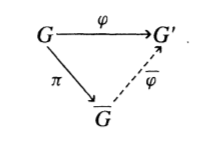
\includegraphics[scale=0.9]{assets/first_iso.png}
\end{center}
Any surjective homomorphism with the kernal $N$ are preimages of elements that have cosets of $N$.

\bigskip 

Recall this lemma, which we may or may not have talked about at some point. 
\begin{lemma}{}{}
    Let $\varphi: G \mapsto G'$ be a surjective homomorphism with kernal $N$. Then, for every $g' \in G'$: 
    \[\varphi^{-1}(g') = \{g \in G \mid \varphi(g) = g'\}\]
    Represents a left/right coset of $N$. 
\end{lemma}
Its proof is as follows: 
\begin{mdframed}
    \begin{proof}
        Since $\varphi$ is surjective, we can pick a $g_1 \in G$ with $\varphi(g_1) = g'$. We claim that $g_1 * N = \varphi^{-1}(g') = N * g$. We show that $g_1 N \subseteq \varphi^{-1}(g')$. For any $n \in N$, we note that $\varphi(g * n) = \varphi(g_1) \cdot \varphi(n) = \varphi(g_1)$. Now we show that $\varphi^{-1}(g') \subseteq g_1 * N$. Pick any $g_2 \in G$ with $\varphi(g_2) = g'$. Then, $\varphi(g_1) = \varphi(g_2)$ implies that $\varphi(g_{1}^{-1} * g_2) = \varphi(g_1)^{-1} \cdot \varphi(g_2) = \id$. So:
        \[g_{1}^{-1} * g_2 \in N \implies g_2 \in g_1 * N\]
        So, we are done.  
    \end{proof}
\end{mdframed}

The following corollary is probably the most useful:
\begin{corollary}{}{}
    Let $\varphi: G \mapsto G'$ be a group homomorphism with kernal $N$ and image $H'$. The quotient group $\overline{G} = G / N$ is isomorphic to the image $H'$. 
\end{corollary}

So, if we need to show that there is an isomorphism of the form: 
\[G / N \cong H\]
All we need to do is: 
\begin{itemize}
    \item Find $\varphi: G \mapsto H$ (a homomorphism). 
    \item Show that $\ker(\varphi) = N$. 
    \item Show that $\im(\varphi) = H$. 
\end{itemize}

\subsubsection{Example 1: Matrices}
Suppose we wanted to show that $GL_{n}(\R) / SL_{n}(\R) \cong \R - \{0\}$. 
\begin{itemize}
    \item Consider $\varphi: GL_{n}(\R) \mapsto \R - \{0\}$, the determinant function.
    \item The kernal of $\varphi$ is all matrices with determinant 1. Thus: 
    \[\ker(\varphi) = SL_{n}(\R) = \{A \in GL_{n}(\R) \mid \det(A) = 1\}\]
    \item The image of $\varphi$ is simply all possible determinants; that is: 
    \[\im(\varphi) = \R - \{0\}\]
\end{itemize}
Therefore, $GL_{n}(\R) / SL_{n}(\R) \cong \R - \{0\}$. 

\subsubsection{Example 2: Permutations}
Suppose we wanted to show that $S_n / A_n \cong \{\pm 1\}$. 
\begin{itemize}
    \item Consider $\varphi: S_n \mapsto \{\pm 1\}$, the sign function. 
    \item By definition, $\ker(\varphi) = A_n$ (recall that the sign of any even permutation is 1). 
    \item By definition, the sign function is surjective if $n \geq 2$. 
\end{itemize}
Therefore, $S_n / A_n \cong \{1\}$. 

\subsubsection{Example 3: Group Itself}
Suppose we wanted to show that $G / G \cong \{1\}$.
\begin{itemize}
    \item Consider $\varphi: G \mapsto G$ by the function $\varphi(g) = 1$, which is a surjective homomorphism.
    \item The kernal of $\varphi$ is all elements $g \in G$ such that $\varphi(g) = 1$. So, this is trivially just $G$. Thus, $\ker(\varphi) = G$. 
    \item Because $\varphi$ is surjective, $\im(\varphi) = \{1\}$.  
\end{itemize}
So, $G / G \cong \{1\}$. 

\subsection{Correspondence Theorem}
We now talk about the correspondence theorem.
\begin{theorem}{Correspondence Theorem}{}
    Let $\varphi: G \mapsto G'$ be a surjective homomorphism with kernal $N$. Then, there is a bijection from the subgroups of $G'$ to the subgroups of $G$ containing $N$ defined by: 
    \[H' \mapsto \varphi^{-1}(H')\]
\end{theorem}

\begin{definition}{Restriction}{}
    Let $\varphi: G \mapsto G'$ be a homomorphism. Let $H$ be a subgroup (not necessarily normal) of $G$. We define: 
    \[\varphi |_{H}: H \mapsto G'\]
    To be the restriction. It can be written as the composition $H \mapsto G \xrightarrow{\varphi} G'$ (the inclusion homomorphism). 
\end{definition}
\textbf{Remarks:}
\begin{itemize}
    \item $\ker\left(\frac{\varphi}{H}\right) = (\ker(\varphi)) \cap H$.
    \item $\im\left(\frac{\varphi}{H}\right) = \varphi(H) = \{\varphi(h) \mid h \in H\}$
\end{itemize}

\subsubsection{Example: Permutations and Sign}
Let $\sigma: S_n \mapsto \{\pm 1\}$ be the sign homomorphism. We define the \underline{alternating group} $A_n$ to be $\ker(\sigma)$. In other words:
\[A_n = \ker(\sigma)\]
Suppose $H$ is a subgroup of $S_n$ of \underline{odd} order. (e.g., $\cyclic{g}$ where $g$ is a cycle of odd length). Then: 
\[|H| = |\ker(\varphi \mid_H)| \cdot \underbrace{\left|\im\left(\frac{\varphi}{H}\right)\right|}_{\substack{\text{Order must divide} \\ \text{order of } \{\pm 1\}}}\]
Here, we note that $\left|\im\left(\frac{\varphi}{H}\right)\right|$ must be 1. This means that $H \subseteq A_n$. 

\subsection{Inverse Image}
We now define an inverse image.
\begin{definition}{Inverse Image}{}
    Let $\varphi: G \mapsto G'$ be a homomorphism. Then, for $H' \subseteq G'$ a subgroup, the \textbf{inverse image} (preimage) is defined by: 
\[\varphi^{-1}(H') = \{g \in G \mid \varphi(g) \in H\}\]
\end{definition}
THis is a subgroup because it has all three characteristics of a subgroup (which we will not show). 

\bigskip

For example, if the homomorphism is $(\Z, +) \mapsto (\Z / \Z n)$, then for any $d$ that divides $n$, the multiples of $d$ in $\Z / \Z n$ form a subgroup whose inverse image in $\Z$ is $\Z d$. For instance, if $d = 4$ and $n = 6$, then the multiples of 4 in $\Z / \Z 6$ are $4(4) = 16 \equiv 2 \mod{6}$. 










\newpage 
\section{Product Groups}
Now, we talk about product groups. 

\subsection{Definition of a Product Group}
\begin{definition}{Product Group}{}
    Let $(G, *)$ and $(G', \cdot)$ be two groups. The product set $G \times G'$, the set of pairs of elements $(a, a')$ with $a \in G$ and $a' \in G'$, can be made into a group by component-wise multiplication; that is, multiplication of pairs is defined by the rule: 
    \[(a, a') \cdot (b, b') = (a * b, a' \cdot b')\]
    This is known as the \textbf{product group}.
\end{definition}
The proof that this is actually a group is as follows:
\begin{mdframed}
    \begin{proof}
        Let $(G, *)$ and $(G', \cdot)$ be two groups. We note that $(\id, \id')$ is the identity (where $\id \in G$ and $\id' \in G'$ are the corresponding identity elements), the inverse of $(a, a')$ is $(a, a')^{-1} = (a^{-1}, (a')^{-1})$, and associativity implicitly applies. Therefore, the product group is a group. 
    \end{proof}
\end{mdframed}

\subsection{Properties of Product Groups}
Now, we focus on some properties of product groups. 

\subsubsection{Prime Order and Isomorphism}
\begin{mdframed}
    \begin{proposition}
        Let $r$ and $s$ be relatively prime integers; that is, $\gcd(r, s) = 1$. A cyclic group of order $rs$ is isomorphic to the product of a cyclic group of order $r$ and a cyclic group of order $s$. 
    \end{proposition}
\end{mdframed}

\subsubsection{Product Groups and Isomorphism}
\begin{mdframed}
    \begin{proposition}
        Let $H$ and $K$ be subgroups of a group $G$ and let $f: H \times K \mapsto G$ be the multiplication map, defined by $f(h, k) = hk$. Its image is the set $HK = \{hk \mid h \in H, k \in K\}$. 
        \begin{enumerate}[(a)]
            \item $f$ is injective if and only if $H \cap K = \{\id\}$ (the identity). 
            \item $f$ is a homomorphism from the product group $H \times K$ to $G$ if and only if the elements of $K$ commute with the elements of $H$: $hk = kh$. 
            \item If $H$ is a normal subgroup of $G$, then $HK$ is a subgroup of $G$. 
            \item $f$ is an isomorphism from the product group $H \times K$ to $G$ if and only if $H \cap K = \{1\}$, $HK = G$, and also $H$ and $K$ are both normal subgroups of $G$. 
        \end{enumerate}
    \end{proposition}
\end{mdframed}

\subsubsection{Order}
\begin{itemize}
    \item The order of a direct product $G_1 \times G_2 \times \dots \times G_n$ is: 
    \[|G_1 \times G_2 \times \dots \times G_n| = |G_1| \cdot |G_2| \cdot \ldots \cdot |G_n|\]
    \item The order of an element $(g, h)$ is: 
    \[|(g, h)| = \lcm(|g|, |h|)\]
    Or, more verbosely, the order of $(g, h)$ is the least common multiple of the orders of $g$ and $h$. 
\end{itemize}









\newpage 
\section{Symmetries and Isometries}
One major application of groups is the idea of symmetries. In fact, groups were invented to analyze symmetries of certain algebraic structures. In this section and the following sections, we will talk about symmetries, isometries, and more. 

\subsection{Types of Symmetries}
Let's begin with a brief introduction on the types of symmetries. 

\subsubsection{Bilateral Symmetry}
Bilaterial symmetry is the property of being divisible into symmetrical halves on either side of a unique plane. For example, consider the following figures: 
\begin{center}
    
\includegraphics[scale=0.8]{assets/bilaterial_sym.png}
\end{center}

\subsubsection{Rotational Symmetry}
Rotational symmetry is essentially the property an object has when it looks the same after some rotation by a partial turn.  
\begin{center}
    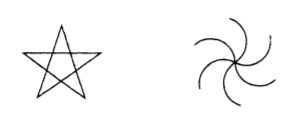
\includegraphics[scale=0.8]{assets/rotational_sym.png}
\end{center}

\subsubsection{Translational Symmetry}
Translational symmetry is the property an object has when a particular translation does not change the object. 
\begin{center}
    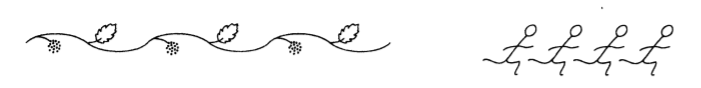
\includegraphics[scale=0.8]{assets/translational_sym.png}
\end{center}
Figures like these are supposed to extend indefinitely in both directions.

\subsubsection{Glide Symmetry}
Glide symmetry is the operation that usually involves reflection in a plane, followed by a translation parallel with that plane. 
\begin{center}
    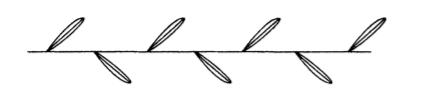
\includegraphics[scale=0.8]{assets/glide_sym.png}
\end{center}
Figures like these are supposed to extend indefinitely in both directions.

\subsubsection{Combining Symmetries}
Of course, we can combine multiple symmetries. For instance, the following wallpaper pattern may have two independent translational symmetries: 
\begin{center}
    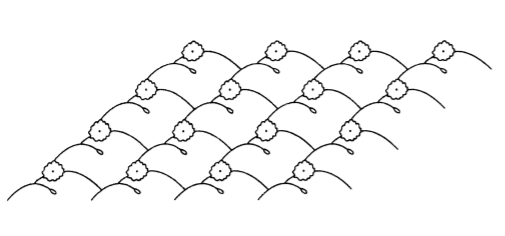
\includegraphics[scale=0.8]{assets/wallpaper.png}
\end{center}
The star from the first few images has bilaterial as well as rotational symmetry. The figure below has both translational and rotational symmetries combined: 
\begin{center}
    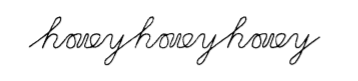
\includegraphics[scale=0.8]{assets/honey.png}
\end{center}


\subsection{Isometries}
Here, we say that a rigid motion of the plane is called an \textbf{isometry}. In particular, these are: 
\begin{itemize}
    \item Translations. 
    \item Rotations. 
    \item Reflections.
    \item Glide Reflections. 
\end{itemize}

We note that all of these rigid motions preserve the overall figure. Of course, there is a more precise definition. 
\begin{definition}{Isometry}{}
    An \textbf{isometry} of $n$-dimensional space $\R^n$ is a distance-preserving map $f$ from $\R^n$ to itself, a map such that for all $u, v \in \R^n$: 
    \[|f(u) - f(v)| = |u - v|\]
    An isometry will map a figure to a congruent figure. 
\end{definition}

\subsubsection{Example: Orthogonal Linear Operations}
An orthogonal operation $\varphi$ is linear, which means that $\varphi(u) - \varphi(v) = \varphi(u - v)$ so that $|varphi(u) - \varphi(v)| = |\varphi(u - v)|$. Additionally, because $\varphi$ is orthogonal, it preserves dot products and lengths. So, $|\varphi(u - v)| = |u - v|$. 

\subsubsection{Example: Translation}
The \emph{translation} $t_a$ by a vector $a$, the map defined by $t_{a}(x) = x + a$, is an isometry.

\subsubsection{Example: Compositions}
The composition of isometries is, of course, an isometry. 

\subsection{Properties of Isometries}
Now, we'll talk about some properties of isometries.

\begin{theorem}{}{}
    The following conditions on a map $\varphi: \R^n \mapsto \R^n$ are equivalent: 
    \begin{itemize}
        \item $\varphi$ is an isometry that fixes the origin: $\varphi(0) = 0$. 
        \item $\varphi$ preserves the dot product: for all $u$ and $v$, $\varphi(v) \cdot \varphi(w) = v \cdot w$.
        \item $\varphi$ is an orthogonal linear operator. 
    \end{itemize}
\end{theorem}

\begin{lemma}{}{}
    Let $x$ and $y$ be points of $\R^n$. If the three dot products $(x \cdot x)$, $(x \cdot y)$, and $(y \cdot y)$ are equal, then $x = y$.  
\end{lemma}

\begin{corollary}{}{}
    Every isometry $f$ of $\R^n$ is the composition of an orthogonal linear operator and a translation. More precisely, if $f$ is an isometry and if $f(0) = a$, then $f = t_{a}\varphi$ where $t_a$ is a translation and $\varphi$ is an orthogonal linear operator. This expression for $f$ is unique. 
\end{corollary}
\textbf{Remark:} To work with the expressions $t_a \varphi$ for isometries, we need to determine the product (i.e. compositions) of two such expressions. Some rules to consider: 
\begin{itemize}
    \item $t_a t_b = t_{a + b}$.
    \item $\varphi t_a = t_{a'}\varphi$ where $a' = \varphi(a)$. 
\end{itemize}
The last relation can be verified like so:
\[\varphi t_{a}(x) = \varphi(x + a) = \varphi(x) + \varphi(a) = \varphi(x) + a' = t_{a'}\varphi(x)\]

\begin{corollary}{}{}
    The set of all isometries of $\R^n$ forms a group that we denoted by $M_n$, with composition of functions as its law of composition. 
\end{corollary}

\begin{mdframed}
    \begin{proof}
        The composition of isometries is an isometry, and the inverse of an isometry is an isometry because orthogonal vectors and translations are invertible. Additionally, if $f = t_a \varphi$, then $f^{-1} = \varphi^{-1} t_{a}^{-1} = \varphi^{-1} t_{-a}$, which is a composition of isometries. 
    \end{proof}
\end{mdframed}

\subsubsection{Homomorphism of the Group of Isometries}
Consider the map $\pi: M_n \mapsto O_n$, defined by dropping the translation part of an isometry $f$. We can write $f$ in the form $f = t_a \varphi$ and define: 
\[\pi(f) = \varphi\]
Here, $O_n$ is the group of isometries preserving the origin. More specifically, it is the group of distance-preserving transformations of an Euclidean space of dimension $n$ that preserves a \emph{fixed point}, where the group operation is (like with $M_n$) composing transformations/isometries. 

\bigskip 

\begin{mdframed}
    \begin{proposition}
        The map $\pi$ is a surjective homomorphism. Its kernal is the set $T = \{t_v\}$ of translations, which is a normal subgroup of $M_n$.
    \end{proposition}    
\end{mdframed}

\begin{corollary}{}{}
    The homomorphism $\pi: M_n \mapsto O_n$ does not change when the origin is shifted by a translation. 
\end{corollary}

\subsubsection{Orientation}
The determinant of an orthogonal operator $\varphi$ on $\R^n$ is $\pm 1$. The operator is said to be:
\begin{itemize}
    \item \textbf{Orientation-preserving} if the determinant is 1. 
    \item \textbf{Orientation-reversing} if the determinant is -1. 
\end{itemize}
Similarly, we note that an orientation-preserving isometry $f$ is one such that, when written in the form $f = t_a \varphi$, the $\varphi$ operator is orientation-preserving. The same can be applied for orientation-reversing. It should be noted that: 
\[\sigma: M_n \mapsto \{\pm 1\}\]
That sends an orientation-preserving isometry to 1 and an orientation-reversing isometry to -1 is a group homomorphism. 


\subsection{Isometries of the Plane}
First, we dneote the group of isometries of the plane by $M$. We choose a coordinate system and use it to identify the plane with the space $\R^2$. Then, we choose as generators the \emph{translations}, the \emph{rotations} about the origin, and the \emph{reflection} about the $e_1$-axis (an axis). We denote the rotation through the angle $\theta$ by $\rho_{\theta}$, and the reflection about the $e_1$-axis by $r$. 

\bigskip 

Essentially, to summarize, we have the following operations:
\begin{enumerate}
    \item \emph{Translation} $t_a$ by a vector $a$. 
    \[t_{a}(x) = x + a = \begin{bmatrix}
        x_1 \\ x_2
    \end{bmatrix} + \begin{bmatrix}
        a_1 \\ a_2
    \end{bmatrix}\]
    \item \emph{Rotation} $\rho_{\theta}$ by an angle $\theta$ about the origin. 
    \[\rho_{\theta}(x) = \begin{bmatrix}
        \cos(\theta) & -\sin(\theta) \\ 
        \sin(\theta) & \cos(\theta)
    \end{bmatrix} \begin{bmatrix}
        x_1 \\ x_2
    \end{bmatrix}\] 
    \item \emph{Reflection} $r$ about the $e_1$-axis.
    \[r(x) = \begin{bmatrix}
        1 & 0 \\ 0 & -1
    \end{bmatrix} \begin{bmatrix}
        x_1 \\ x_2 
    \end{bmatrix}\]
\end{enumerate}
Although we didn't include rotation about a point (other than the origin) or reflections about other lines or glides, every element of $M$ is a product of these isometries. 

\begin{theorem}{}{}
    Let $m \in M$ be an isometry of the plane. Then, for a uniquely determined vector $v$ and an angle $\theta$ that is possibly zero: 
    \[m = t_v \rho_{\theta}\]
    \[m = t_v \rho_{\theta} r\] 
\end{theorem}
\textbf{Remark:} An isometry of the form $t_v \rho_{\theta}$ preserves orientation while $t_v \rho_{\theta} r$ reverses orientation. 

\begin{mdframed}
    \begin{proof}
        We know that any isometry $m$ is written uniquely in the form $m = t_v \varphi$ where $\varphi$ is an orthogonal operator. In $\R^2$, those orthogonal linear operators are the rotations $\rho_{\theta}$ about the origin and the reflection about lines through the origin. The reflections have the form $\rho_{\theta} r$. 
    \end{proof}
\end{mdframed}

Computation in $M$ can be done using the symbols $t_v$, $\rho_{\theta}$, and $r$, using the following rules for composing them: 
\begin{itemize}
    \item $\rho_{\theta} t_v = t_{v'} \rho_{\theta}$ where $v' = \rho_{\theta}(v)$. 
    \item $rt_v = t_{v'}r$ where $v' = r(v)$. 
    \item $r\rho_{\theta} = \rho_{-\theta} r$. 
    \item $t_v t_w = t_{v + w}$. 
    \item $\rho_{\theta_1}\rho_{\theta_2} = \rho_{\theta_1 + \theta_2}$.
    \item $rr = 1$. 
\end{itemize}

\begin{theorem}{}{}
    Every isometry of the plane has one of the following forms: 
    \begin{enumerate}[(a)]
        \item Orientation-preserving isometries. 
        \begin{itemize}
            \item Translation: a map $t_v$ that sends $p \rightsquigarrow p + v$.
            \item Rotation: rotation of the plane through a nonzero angle $\theta$ about some point.  
        \end{itemize}

        \item Orientation-reversing isometries: 
        \begin{itemize}
            \item Reflection: a bilaterial symmetry about a line $\ell$. 
            \item Glide Reflection (or \emph{glide} for short): reflection about a line $\ell$, followed by a translation by a nonzero vector parallel to $\ell$. 
        \end{itemize}
    \end{enumerate}
\end{theorem}

\subsection{Finite Group of Orthogonal Operators on the Plane}
\begin{theorem}{}{}
    Let $G$ be a finite subgroup of the orthogonal group $O_2$. There is an integer $n$ such that $G$ is one of the following groups: 
    \begin{itemize}
        \item $C_n$: the \emph{cyclic group} of order $n$ generated by the rotation $\rho_{\theta}$ where $\theta = 2\pi / n$. 
        \item $D_n$: the \emph{dihedral group} of order $2n$ generated by two elements: the rotation $\rho_{\theta}$, where $\theta = 2\pi / n$, and a reflection $r$ about a line $\ell$ through the origin. 
    \end{itemize}
\end{theorem}
\textbf{Remark:} Recall that $O_n$ is the group of isometries that preserve a fixed point (in our case, most of the time, the origin). So, it makes sense to drop the translation part of the isometry. 

\subsubsection{Dihedral Groups: An Introduction}
As mentioned, the dihedral group is comprised of rotations $\rho_{\theta}$ and a reflection $r'$. Let us define $x = \rho_{\theta}$ and $y = r$. 

\begin{mdframed}
    \begin{proposition}
        The dihedral group $D_n$ has order $2n$. It is generated by two elements $x$ and $y$ that satisfy the relations: 
        \[x^n = \id \qquad y^2 = \id \qquad yx = x^{-1} y\]
        The elements of $D_n$ are: 
        \[\{\id, x, x^2, \dots, x^{n - 1}, y, xy, x^{2}y, \dots, x^{n - 1}y\}\]
    \end{proposition}
\end{mdframed}
We can write more relations. In particular: 
\[xyxy = \id \qquad yx = x^{n - 1}y \qquad xy = yx^{-1}\]

\textbf{Remarks:} 
\begin{itemize}
    \item Rotations ($x$) will always have order $n$. 
    \item Reflections ($y$ or $x^a y$ for some $a$) will always have order 2. 
\end{itemize}

\begin{corollary}{}{}
    The dihedral group $D_3$ and the symmetric group $S_3$ are isomorphic. 
\end{corollary}
\begin{mdframed}
    \begin{proof}
        Since these groups are sufficiently small enough as both have order 6, we can count the orders of each element. In particular, for $D_3$: 
        \begin{center}
            \begin{tabular}{c|c|c}
                \textbf{Order} & \textbf{Elements} & \textbf{Count} \\ 
                \hline 
                1 & $\id$ & 1 \\ 
                2 & $xy$, $y$, $x^2 y$ & 3 \\ 
                3 & $x$, $x^2$ & 2
            \end{tabular}
        \end{center}

        And for $S_3$: 
        \begin{center}
            \begin{tabular}{c|c|c}
                \textbf{Order} & \textbf{Elements} & \textbf{Count} \\ 
                \hline 
                1 & $\id$ & 1 \\ 
                2 & $(12)$, $(13)$, $(23)$ & 3 \\ 
                3 & $(123)$, $(132)$ & 2
            \end{tabular}
        \end{center}
        
        Since both groups have the same number of elements with the same number of orders, they are isomorphic to each other. 
    \end{proof}
\end{mdframed}
\textbf{Remarks:}
\begin{itemize}
    \item For $n > 3$, $S_n$ and $D_n$ are no longer isomorphic since $D_n$ has order $n!$ while $S_n$ has order $n!$. 
    \item When $n \geq 3$, the elements of the dihedral group $D_n$ are orthogonal operators that carry a regular $n$-sided polygon $\triangle$ to itself: the group of symmetries of $\triangle$. 
    \item $D_1$ and $D_2$ are too small to be symmetry groups of an $n$-gon in the usual sense.
    \begin{itemize}
        \item In particular, we can think of $D_1$ as the group $\{\id, r\}$ of two elements, or a cyclic group. 
        \item $D_2$ contains the four elements $\{\id, \rho, r, \rho r\}$ where $\rho$ is the rotation with angle $\pi$ and $\rho r$ is the reflection about the vertical axis, and is isomorphic to the Klein four group. 
    \end{itemize}
\end{itemize}

\subsubsection{Discrete Subgroups}
\begin{definition}{Discrete Subgroup}{}
    A subgroup $\Gamma$ of the additive group $(\R, +)$ is called \textbf{discrete} if there is a (small) positive real number $\epsilon$ such that every nonzero element $c$ of $\Gamma$ satisfies the property $|c| \geq \epsilon$. 
\end{definition}

\subsubsection{Fixed Point Theorem}
\begin{theorem}{Fixed Point Theorem}{}
    Let $G$ be a finite group of isometries of the plane. There is a point in the plane that is fixed by every element of $G$, a point $p$ such that $g(p) = p$ for all $g \in G$. 
\end{theorem}


\subsection{Discrete Groups of Isometries}
\begin{definition}{Discrete Group}{}
    A group $G$ of isometries of the plane $P$ is \textbf{discrete} if it does not contain arbitrarily small translations or rotations. More precisely, $G$ is discrete if there is a positive real number $\epsilon$ so that: 
    \begin{enumerate}[(i)]
        \item If an element of $G$ is the translation by a nonzero vector $a$, then the length of $a$ is at least $\epsilon$: $|a| \geq \epsilon$.
        \item If an element of $G$ is the rotation through a nonzero angle $\epsilon$ about some point of the plane, then the absolute value of $\theta$ is at least $\epsilon$: $|\theta| \geq \epsilon$.
    \end{enumerate}
\end{definition}
\textbf{Remark:} Since the translation vectors and the rotation angles form different sets, it might seem more appropriate to have separate lower bounds for them. However, in this definition, we do not care about the best bounds for the vectors and the angles, so we choose $\epsilon$ small enough to take care of both at the same time. 

\bigskip

There are three main tools for analyzing a discrete group $G$: 
\begin{itemize}
    \item The translation group $L$, a subgroup of the group $V$ of translation vectors. 
    \item The point group $\overline{G}$, a subgroup of the orthogonal group $O_2$. 
    \item An operation of $\overline{G}$ on $L$. 
\end{itemize}

\subsubsection{Translation Group}
The translation group $L$ of $G$ is the set of vectors $v$ such that the translation $t_v$ is in $G$: 
\[L = \{v \in G \mid t_v \in G\}\]
Since $t_v t_w = t_{v + w}$ and $t_{v}^{-1} = t_{-v}$, it follows that $L$ is a subgroup is the additive group $V^+$ of all translation vectors. The bound $\epsilon$ on translations in $G$ bounds the lengths of the vectors in $L$. 

% TODO 











\newpage
\section{Group Action (Operations)}
We now focus on the aspect of groups as the symmetries of sets, of which we use group actions to formalize. 

\subsection{Definition of a Group Action}
\begin{definition}{Group Action}{}
    If $(G, \cdot)$ is a group with identity element $\id$ and $X$ is a set, then a left \textbf{group action} $m$ of $G$ on $X$ is a function: 
    \[m: G \times X \mapsto X \qquad (g, x) \mapsto g * x\]
    That satisfies the following two axioms: 
    \begin{itemize}
        \item \underline{Identity:} For all $x \in X$,
        \[m(\id, x) = x\]
        \item \underline{Associativity:} For $g_1, g_2 \in G$ and $x \in X$, 
        \[m(g_1, \alpha(g_2, x)) = m(g_1 \cdot g_2, x)\]
    \end{itemize}

    When it's clear that we're performing a group action, we can shorten the axioms as follows: 
    \begin{itemize}
        \item \underline{Identity:} For all $x \in X$,
        \[\id * x = x\]
        \item \underline{Associativity:} For all $g_1, g_2 \in G$ and $x \in X$, 
        \[g_1 * (g_2 * x) = (g_1 \cdot g_2) * x\]
    \end{itemize}

    In this sense, we say that $G$ acts on $X$ with $m$ and write $G \curvearrowright X$.
\end{definition}

\subsubsection{Example: Symmetric Group}
Take $G = S_n$ and $X = \{1, 2, \dots, n\}$. Then, for some $\sigma \in S_n$ and $i \in X$: 
\[\sigma * i = \sigma(i)\]
Here, we apply $\sigma$ to $x$, or we say that $\sigma$ acts on $x$. 

\begin{mdframed}
    \begin{proof}
        Here, we show that this a group action. 
        \begin{itemize}
            \item \underline{Identity:}
            \[\id * i = \id(i) = i\]

            \item \underline{Associativity:}
            \begin{equation*}
                \begin{aligned}
                    \sigma_1 * (\sigma_2 * i) &= \sigma_1 * \sigma_{2}(i) \\ 
                        &= \sigma_{1}(\sigma_{2}(i)) \\ 
                        &= (\sigma_{1}\sigma_{2})(i) \\ 
                        &= \sigma_{1}\sigma_{2} * i
                 \end{aligned}
            \end{equation*}
        \end{itemize}
        So, we are done. 
    \end{proof}
\end{mdframed}

\subsubsection{Example: Group on Itself via Multiplication}
Suppose $(G, \cdot)$ is a group. Then, $G$ acts on $G$ by left multiplication. Take $g \in G$ and $x \in G$. Then:  
\[g * x = g \cdot x\]

\subsubsection{Example: Group on Itself via Conjugation}
Suppose $(G, \cdot)$ is a group. Then, $G$ acts on $G$ by conjugation. Take $g \in G$ and $x \in G$. Then:  
\[g * x = g \cdot x \cdot g^{-1}\]

\begin{mdframed}
    \begin{proof}
        Here, we show that this is a group action. 
        \begin{itemize}
            \item \underline{Identity:}
            \[\id * x = \id \cdot x \cdot \id^{-1} = x\]

            \item \underline{Associativity:}
            \begin{equation*}
                \begin{aligned}
                    g_1 * (g_2 * x) &= g_1 * (g_2 \cdot x \cdot g_{2}^{-1}) \\ 
                        &= g_1 \cdot (g_2 \cdot x \cdot g_{2}^{-1}) \cdot g_{1}^{-1} \\ 
                        &= (g_1 \cdot g_2) \cdot x \cdot (g_{2}^{-1} \cdot g_{1}^{-1}) \\ 
                        &= (g_1 \cdot g_2) \cdot x \cdot (g_1 \cdot g_2)^{-1} \\ 
                        &= (g_1 \cdot g_2) * x
                \end{aligned}
            \end{equation*}
        \end{itemize}
        So, we are done. 
    \end{proof}
\end{mdframed}

\subsection{Orbit}
Given an operation of a group $G$ on a set $X$, an element $x \in X$ will be sent to various other elements by the group action. We collect together these elements, obtaining a subset called the orbit. 
\begin{definition}{Orbit}{}
    Suppose $G$ acts on $X$. Then, the \textbf{orbit} of $x \in X$ is defined by: 
    \[O_x = \{x' \in X \mid x' = g * x \text{ for some } g \in G\} = \{g * x \mid g \in G\}\] 
\end{definition}

The orbits for a group action are equivalence classes for the equivalence relation: 
\[x \sim y \text{ if } y = g * x \text{ for some } g \in G\]
Since they are equivalence classes, the orbits partition the set $X$. If $X$ consists of just one orbit, then the action of $G$ is called \textbf{transitive}; this means that every element of $X$ is carried to every other one by some element of the group.

\subsubsection{Example: Symmetric Group}
Suppose we're asked to describe the orbits of the group operation of $S_n$ on $\{1, 2, \dots, n\}$ by: 
\[\sigma * i = \sigma(i)\]
\begin{mdframed}
    \begin{proof}
        Consider the orbits of the group operation $S_n$ on $\{1, 2, \dots, n\}$ by $\sigma * i = \sigma(i)$. Then, for $\sigma \in S_n$, we have:  
        \[O_{i} = \{\sigma(i) \mid \sigma \in S_n\} = \{1, 2, \dots, n\}\]
        In this case, we consider the action of $S_n$ to be transitive. Consider the following permutation: 
        \[\sigma = (i, k) \in S_n\]
        If $i \in \{1, 2, \dots, n\}$ is our input and $k$ is the number that we're trying to find, then we note that $i$ maps to $k$ so that there is always a way to get some $k \in \{1, 2, \dots, n\}$. 
    \end{proof}
\end{mdframed}

As an example, suppose we have the group $S_4$ with the set $S = \{1, 2, 3, 4\}$. Then, you are able to get every element in $S$ like so: 
\begin{itemize}
    \item $\sigma = (2, 4) \in S_4$. Then, $\sigma(2) = 4$. In other words, 2 maps to 4.
    \item $\sigma = (2, 3) \in S_4$. Then, $\sigma(2) = 3$. In other words, 2 maps to 3.
    \item $\sigma = (1) \in S_4$. Then, $\sigma(2) = 2$. In other words, 2 maps to 2.
    \item $\sigma = (2, 1) \in S_4$. Then, $\sigma(2) = 1$. In other words, 2 maps to 1.
\end{itemize}

\subsubsection{Example: Symmetric Group, Tuple Pair}
Suppose we're asked to describe the orbits of the group operation of $S_n$ on $\{1, 2, \dots, n\}$ by: 
\[\sigma * (i_1, i_2) = (\sigma(i_1), \sigma(i_2))\]

\begin{mdframed}
    \begin{proof}
        We claim that the orbits of the group operation mentioned above are: 
        \[O_{(a, b)} = \text{All tuples such that both elements are unique, i.e. not the same.}\]
        \[O_{(a, a)} = \text{All tuples such that both elements are the same.}\]
        To show that this is the case, we can work with $O_a$ and $O_b$ individually. For some $a \in \{1, 2, \dots, n\}$, we note that $O_a = \{1, 2, \dots, n\}$ by the same logic we used in the previous example. We can do the same with $b$. If $a \neq b$, then it follows that $O_{(a, b)}$ will generate all unique possibilities of $(c, d)$ such that $c, d \in \{1, 2, \dots, n\}$ where $c \neq d$. But, suppose $a = b$. Then, the resulting orbit will be all tuples where the first and second elements are the same. Taking the union of both orbits, we have: 
        \[O_{(a, b)} \cup O_{(a, a)} = \{1, 2, \dots, n\}^2\]
        As expected. 
    \end{proof}
\end{mdframed}

\subsubsection{Example: Conjugation}
Consider again the example of conjugation. In particular, if $G$ acts on $G$ by conjugation, then the orbit is defined as: 
\begin{equation*}
    \begin{aligned}
        O_{x} &= \{g * x \mid g \in G\} \\
            &= \{g \cdot x \cdot g^{-1} \mid g \in G\} \\ 
            &= C_x
    \end{aligned}
\end{equation*}
This is the set of all conjugates of $x$, and the set of all conjugates of $x$ is called the conjugacy class of $x$.

\subsection{Stabilizer}
\begin{definition}{Stabilizer}{}
    The \textbf{stabilizer} of an element $x \in X$ is the set of group elements that leave $x$ fixed. It is a \emph{subgroup} of $G$ that we denoted by $G_x$:
    \[G_x = \{g \in G \mid g * s = s\}\] 
\end{definition}

\begin{mdframed}
    \begin{proposition}
        Let $X$ be a set on which a group $G$ acts on. Let $x \in X$ and let $H$ be the stabilizer of $x$. Then: 
        \begin{enumerate}[(a)]
            \item If $a$ and $b$ are elements of $G$, then $a * s = b * s$ if and only if $a^{-1} \cdot b \in H$, and this is true if and only if $b$ is in the coset $aH$. 
            \item Suppose that $a * s = s'$. The stabilizer $H'$ of $s'$ is a conjugate subgroup: 
            \[H' = aHa^{-1} = \{g \in G \mid g = aha^{-1} \text{ for some } h \in H\}\]
        \end{enumerate}
    \end{proposition}
\end{mdframed}

\subsubsection{Example: Permutations}
Consider the permutation group $S = \{(1), (12), (34), (12)(34)\}$ and the set $\{1, 2, 3, 4\}$. Then: 
\[G_1 = \{g \in G \mid g(1) = 1\} = \{(1), (34)\}\]
\[G_2 = \{g \in G \mid g(2) = 2\} = \{(1), (34)\}\]
\[G_3 = \{g \in G \mid g(3) = 3\} = \{(1), (12)\}\]
\[G_4 = \{g \in G \mid g(4) = 4\} = \{(1), (12)\}\]

\begin{mdframed}
    \begin{proposition}
        Let $X$ be a set on which a group $G$ operates, and let $x \in X$ and let $H$ be a stabilizer of $x$.
        \begin{enumerate}[(a)]
            \item If $a, b \in G$, then $a * x = b * x$ if and only if $a^{-1}b \in H$, and this is true if and only if $b \in aH$. 
            \item Suppose that $a * x = x'$. The stabilizer $H'$ of $x'$ is a \emph{conjugate subgroup}:
            \[H' = aHa^{-1} = \{g \in G \mid g = aha^{-1} \text{ for some } h \in H\}\]
        \end{enumerate}
    \end{proposition}
\end{mdframed}

\subsection{Operation on Cosets}
Let $H$ be a subgroup of $G$. The left cosets $aH$ partition $G$. We often denote the set of left cosets of $H$ in $G$ by $G / H$, copying this from the notation used for quotient groups when the subgroup is normal, and we used the bracket notation $[C]$ or $\overline{a}$ ($a$ being a representative element for a coset) for a coset $C$, when it is considered as an element of the set $G / H$. \textbf{Note} that the set of cosets $G / H$ is not a group unless $H$ is a normal subgroup. However, the group $G$ operates on $G / H$ in a natural way. 

\bigskip 

\subsubsection{The Operation}
If $g \in G$ and $C$ is a coset, then $g[C]$ is defined to be the coset $[gC]$, where $gC = \{gc \mid c \in C\}$. Thus, if $[C] = [aH]$, then $g[C] = [gaH]$. 

\begin{mdframed}
    \begin{proposition}
        Let $H$ be a subgroup of a group $G$. 
        \begin{itemize}
            \item The operation of $G$ on the set $G / H$ of cosets is transitive. 
            \item The stabilizer of the coset $[H]$ is the subgroup $H$. 
        \end{itemize}
    \end{proposition}
\end{mdframed}

\subsubsection{Example: Symmetric Group}
Let $G = S_3$. Note that $x = (123)$ and $y = (12)$. Then, let $H = \{1, y\}$. Its left cosets are: 
\[C_1 = H = \{1, y\}\]
\[C_2 = xH = \{x, xy\}\]
\[C_3 = x^2 H = \{x^2, x^2 y\}\]
Here, $G$ operates on the set of cosets $G / H = \{[C_1], [C_2], [C_3]\}$. The elements $x$ and $y$ operate in the same way as on the set $\{1, 2, 3\}$: 
\[m_x \longleftrightarrow (123)\]
\[m_y \longleftrightarrow (23)\]
For example, $yC_2 = \{yx, yxy\} = \{x^2 y, x^2\} = C_3$. 

\subsubsection{Example: Symmetric Group on Power Set}
If $S_3$ operates on $[3] = \{1, 2, 3\}$, then $S_3$ operates on $\mathcal{P}([3])$. For instance, take $\sigma = (123) \in S_3$. Then: 
\[\sigma * \emptyset = \emptyset\]
\[\sigma * \{1\} = \{2\}\]
\[\sigma * \{1, 3\} = \{2, 1\}\]
\[\sigma * \{1, 2, 3\} = \{2, 3, 1\} = \{1, 2, 3\}\]

\subsection{The Counting Formula}
Let $H$ be a subgroup of a finite group $G$. All cosets of $H$ in $G$ have the same number of elements, and with the notation $G / H$ for the set of cosets, the order $|G / H|$ is what is called the index $[G: H]$ of $H$ in $G$. The counting formula from a few sections ago, then, stated: 
\[|G| = |H| \cdot |G / H|\]

A similar formula exists for orbits of any group operation. 

\begin{mdframed}
    \begin{proposition}
        Let $X$ be a finite set on which a group $X$ operates on, and let $G_x$ and $O_x$ be the stabilizer and orbit of an element $x \in X$, respectively. Then: 
        \[|G| = |G_s| \cdot |O_s|\]
        \[\text{(Order of $G$)} = \text{(Order of Stabilizer)} \cdot \text{(Order of Orbit)}\]
    \end{proposition}
\end{mdframed}
The order of the orbit is equal to the index of the stabilizer. 
\[|O_s| = [G: G_s]\]
This divides the order of the group. There is one such formula for every $x \in X$. 

\bigskip 

Another formula uses the partition of the set $X$ into orbits to count its elements. This formula is: 
\[|X| = |O_1| + |O_2| + \dots + |O_n|\]
Where $1, 2, \dots, n$ are for labeling purposes. 


\subsection{Operations on Subsets}
Suppose that $G$ operates on a set $X$. If $U$ is a subset of $X$ of order $r$, then: 
\[gU = \{gu \mid u \in U\}\]
Is another subset of order $r$. This allows us to define an operation of $G$ on the set of subsets of order $r$ of $S$.


\subsection{Finite Subgroups of the Rotation Group}
We will now apply the Counting Formula to classify the finite subgroups of $SO_3$, the group of rotations of $\R^3$. 

\begin{theorem}{}{}
    A finite subgroup of $SO_3$ (the group of all rotations about the origin of $\R^3$ under the operation of composition) is one of the following groups: 
    \begin{itemize}
        \item $C_k$: The cyclic group of rotations by multiples of $2\pi / k$ about a line, with $k$ arbitrary. 
        \item $D_k$: The dihedral group of symmetries of a regular $k$-gon, with $k$ arbitrary.
        \item $T$: The tetrahedral group of 12 rotational symmetries of a tetrahedron.
        \item $O$: The octahedral group of 24 rotational symmetries of a cube or an octahedron. 
        \item $I$: The icosahedral group of 60 rotational symmetries of a dodecahedron or an icosahedron.  
    \end{itemize}
\end{theorem}
\textbf{Remarks:}
\begin{itemize}
    \item This is what a tetrahedron (i.e. triangular pyramid) looks like: 
    \begin{center}
        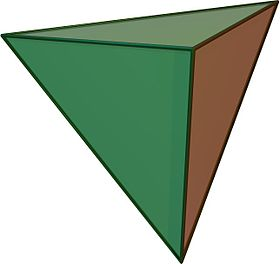
\includegraphics[scale=0.3]{assets/tetra.jpg}
    \end{center}

    \item This is what an octahedron looks like: 
    \begin{center}
        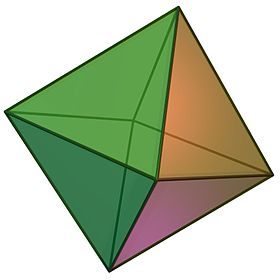
\includegraphics[scale=0.3]{assets/octo.jpg}
    \end{center}
    
    \item This is what an dodecahedron looks like: 
    \begin{center}
        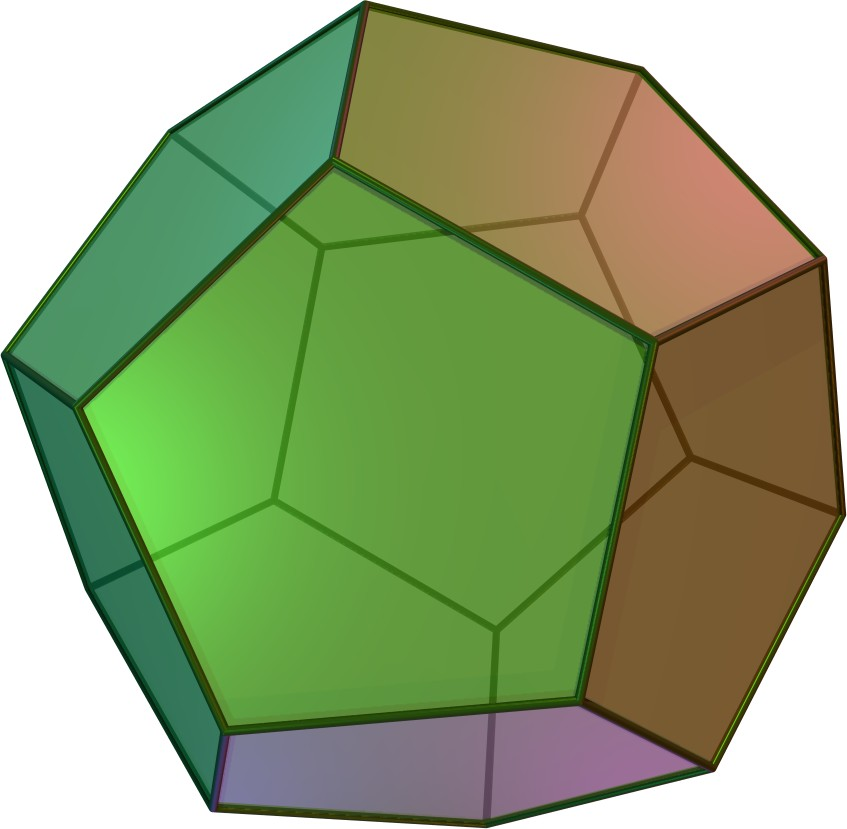
\includegraphics[scale=0.1]{assets/dodeca.jpg}
    \end{center}
    
    \item This is what an icosahedron looks like: 
    \begin{center}
        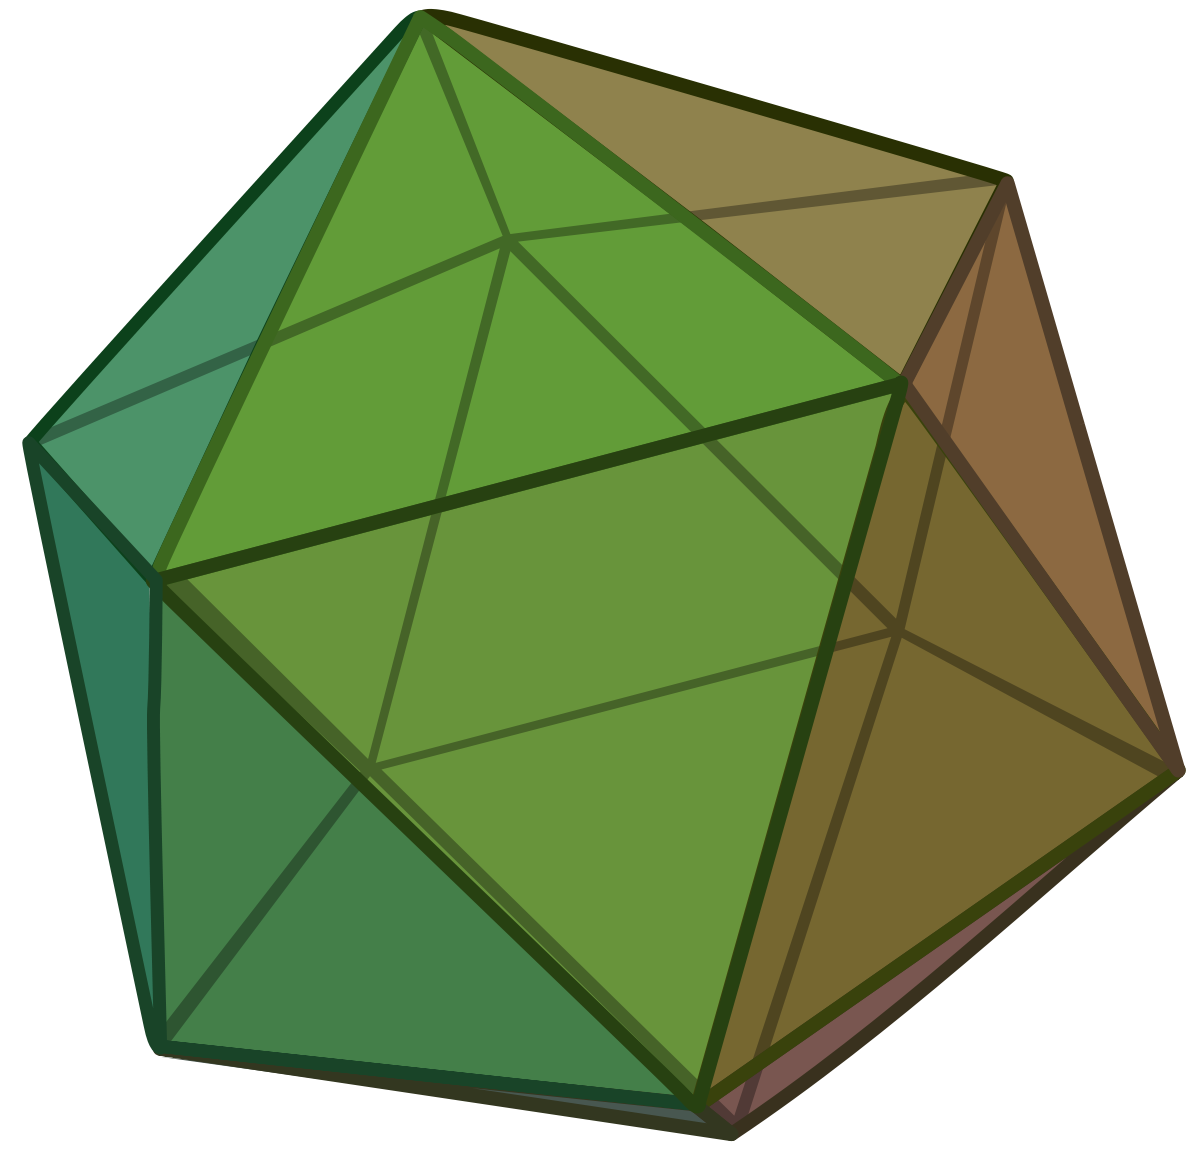
\includegraphics[scale=0.07]{assets/icosa.png}
    \end{center}
\end{itemize}

\begin{definition}{Pole}{}
    For $g \in SO_3$, call $p \in \mathbb{S}^2$ (the unit sphere) a \textbf{pole} of $g$ if $g * p = p$. 
\end{definition}
\textbf{Remarks:}
\begin{itemize}
    \item If $g \neq \id$, then $g$ has two distinct poles. 
    \item If $G \subseteq SO_3$ is a subgroup, we say $p$ is a pole of $G$ if $p$ is a pole of some $g \in G - \{\id\}$. 
\end{itemize} 

\begin{lemma}{}{}
    The set $P$ of poles of $G$ is a union of $G$-orbits. 
\end{lemma}
\textbf{Remark:} This is an abstract way of saying that vertices are sent to vertices, center of faces are sent to center of faces, and center of edges are sent to center of edges. 

\begin{lemma}{}{}
    Let $|G| = N$ and $|G_p| = r_p$. Then: 
    \[\sum_{i = 1}^{k} \left(1 - \frac{1}{r_i}\right) = 2 - \frac{2}{N}\]
    Where $P = O_1 \cup O_2 \cup \dots \cup O_k$ is a union of $k$ $G$-orbits and $r_i = r_p$ for some $p \in O_i$. 
\end{lemma}

















\newpage 
\section{More Applications of Group Theory}
Here, we will talk about several important topics. A lot of these will involve conjugation (once again). 

\subsection{Cayley's Theorem}
\begin{theorem}{Cayley's Theorem}{}
    Every finite group is isomorphic to a subgroup of a permutation group. A group of order $n$ is isomorphic to a subgroup of the symmetric group $S_n$. 
\end{theorem}

\subsection{The Class Equation}
\begin{definition}{Centralizer}{}
    The stabilizer of an element $x \in G$ for the operation of conjugation is called the \textbf{centralizer} of $x$. It is often denoted by $Z(x)$: 
    \[Z(x) = \{g \in G \mid gx = xg\}\]
    The centralizer of $x$ is the set of elements that commute with $x$. 
\end{definition}
\textbf{Remarks:}
\begin{itemize}
    \item The centralizer of an element $g \in G$ is a \emph{subgroup} of $G$. 
    \item This should not be confused with the center of a group $Z(G)$, which is the set of elements that commute with every element of the group: 
    \[Z(G) = \{z \in G \mid zy = yz \text{ for all } y \in G\}\]
\end{itemize}

\begin{definition}{Conjugacy Class}{}
    The orbit for $x$ for conjugation is called the \textbf{conjugacy class} of $x$, and is often denoted by $C(x)$. It consists of all of the conjugates $g \cdot x \cdot g^{-1}$:
    \[C(x) = \{gxg^{-1} \mid g \in G\}\]
\end{definition}

The counting formula tells us that: 
\[|G| = |Z(x)| \cdot |C(x)|\]
\[|G| = |\text{Centralizer}| \cdot |\text{Conjugacy Class}|\]

\begin{mdframed}
    \begin{proposition}
        \begin{enumerate}[(a)]
            \item The centralizer $Z(x)$ of an element $x \in G$ contains $x$, and it contains the center $Z$. 
            \item An element $x \in G$ is in the center if and only if its centralizer $Z(x)$ is the whole group $G$, and this happens if and only if the conjugacy class $C(x)$ consists of the element $x$ alone. 
        \end{enumerate}
    \end{proposition}
\end{mdframed}

Since the conjugacy classes are orbits for a group operation, they partition the group. This fact gives us the \textbf{class equation} of a finite group: 
\[|G| = \sum_{\substack{\text{Conjugacy} \\ \text{\text{Classes } C}}} |C|\]
If we number the conjugacy classes, writing them as $C_1, C_2, \dots, C_k$, then the class equation reads: 
\[|G| = |C_1| + |C_2| + \dots + |C_k|\]
A few facts to remember: 
\begin{itemize}
    \item The conjugacy class of the identity element $\id$ consists of that element alone, so it seems natural to list that class first. Thus, $|C_1| = 1$> 
    \item If there are any other occurrences of 1 on the right side of the class equation, then those correspond to the elements of the center $Z$ of $G$. 
    \item Each term on the right side divides the left side since it is the order of an orbit. In other words, the numbers on the right side of the class equation divide the order of the group. 
    \item At least one of the numbers on the right side must be equal to 1 (the identity conjugacy class). 
\end{itemize}

\subsubsection{Example: Class Equation of Symmetric Group of 4 Elements}
Find the class equation of the symmetric group of 4 elements, or $S_4$.

\begin{mdframed}
    \begin{proof}
        We note that cycle type determines conjugacy classes. We know that $S_4$ has the following cycle structures (i.e. conjugacy classes):
        \begin{center}
            \begin{tabular}{c|c}
                \textbf{Cycle Structure} & \textbf{Size of Conjugacy Class} \\ 
                \hline 
                \code{(a)(b)(c)(d)} & 1 \\ 
                \code{(ab)(c)(d)}  & 6 \\ 
                \code{(ab)(cd)} & 3 \\ 
                \code{(abc)(d)} & 8 \\ 
                \code{(abcd)} & 6 
            \end{tabular}
        \end{center}
        So, the class equation for $S_4$ is: 
        \[|S_4| = 1 + 6 + 3 + 8 + 6\]
        And we are done. 
    \end{proof}
\end{mdframed}

\subsubsection{Example: Class Equation of Dihedral Group of 5 Elements}
Find the class equation for the dihedral group of 5 elements, or $D_5$. 

\begin{mdframed}
    \begin{proof}
        Recall that $D_5 = \{\id, x, x^2, x^3, x^4, y, xy, x^2 y, x^3 y, x^4 y\}$, where $x$ is a rotation and $y$ is a reflection. 
        \begin{itemize}
            \item First, the identity element will always be in its own conjugacy class. So, $C(\id) = \{\id\}$ and $|C(\id)| = 1$. 
            
            \item Let's now consider $C(x)$. Iterating over every element in $D_5$, we find that all rotations will give us back $x$. Let's consider different variations of reflections.   
            \[y \cdot x \cdot y^{-1} = yyx = x\]
            \[xy \cdot x \cdot (xy)^{-1} = xy \cdot x \cdot y^{-1} x^{-1} = xy \cdot x \cdot y x^{-1} = xy y x^{-1} x^{-1} = x x^{-2} = x^{-1} = x^4\]
            Omitting the rest of the computations, we find that: 
            \[C(x) = \{x, x^4\} \qquad |C(x)| = 2\]
            
            \item We now consider $C(x^2)$. Again, iterating over every element in $D_5$, we find that all rotations will give us back $x^2$. Let's consider different variations of reflections. 
            \[xy \cdot x^2 \cdot (xy)^{-1} = xy \cdot x^2 \cdot y^{-1} x^{-1} = xy \cdot x^2 \cdot y x^{-1} = xy yx^{-2} x^{-1} = x x^{-2} x^{-1} = x^{-2} = x^{3}\]
            Omitting the rest of the computations, we find that: 
            \[C(x^2) = \{x^2, x^3\} \qquad |C(x^2)| = 2\]
        \end{itemize}
        At this point, we've found all conjugacy classes for rotations only. This is because: 
        \[C(x) = C(x^4) \qquad C(x^2) = C(x^3)\]
        So, we now consider different variations of reflections. 
        \begin{itemize}
            \item Let's consider $C(y)$. Iterating over every element in $D_5$ gives us: 
            \[x \cdot y \cdot x^{-1} = xxy = x^2 y\]
            \[x^2 \cdot y \cdot x^{-2} = x^2 x^2 y = x^4 y\]
            \[x^3 \cdot y \cdot x^{-3} = x^3 x^3 y = x^6 y = xy\]
            \[x^4 \cdot y \cdot x^{-4} = x^4 x^4 y = x^8 y = x^3 y\]
            We no longer need to check the rest of the reflections since, if we did, we would end up getting the same result from the computations we just did. Therefore: 
            \[C(y) = \{y, xy, x^2 y, x^3 y, x^4 y\} \qquad |C(y)| = 5\]
        \end{itemize}
        We have now found which conjugacy classes each element in $D_5$ goes to. It follows that the class equation for $D_5$ is: 
        \[|D_5| = |C(\id)| + |C(x)| + |C(x^2)| + |C(y)| = 1 + 2 + 2 + 5\]
        And so we are done. 
    \end{proof}
\end{mdframed}

\subsubsection{Example: Valid and Invalid Class Equations}
Rule out as many class equations for a group of order 10 as possible:
\[1 + 1 + 1 + 2 + 5 \qquad 1 + 2 + 2 + 5 \qquad 1 + 2 + 3 + 4 \qquad 1 + 1 + 2 + 2 + 2 + 2\]

\begin{mdframed}
    \begin{proof}
        We begin with $1 + 1 + 1 + 2 + 5$. We note that there are 3 conjugacy classes with 1 element each; these are the center (note that the identity is in the center), so $|Z| = 3$. Since the center of a group is a subgroup, we note that this means that the center has order 3. However, by Lagrange's Theorem, 3 does not divide 10 so the center of this group cannot be 3. 

        \bigskip

        We now turn our attention to $1 + 2 + 2 + 5$. We just proved that this was actually the conjugacy class for $D_5$, so nothing needs to be done here. 

        \bigskip

        Now, let's look at $1 + 2 + 3 + 4$. We note that there is a conjugacy class of 3 elements; however, rememeber that all orders of each conjugacy class must divide the order of the group. As 3 does not divide 10, we can rule this out. 

        \bigskip

        Finally, we look at $1 + 1 + 2 + 2 + 2 + 2$. Note that there are 2 conjugacy classes with 1 element each; these are the center of the group, so $|Z| = 2$. Recall that $Z$ is a normal subgroup, so $G / Z$ has order $|G| / |Z| = 5$, which is cyclic as 5 is prime. If $G/Z$ is cyclic, then $G$ must be abelian. But, abelian groups can only have the class equation $1 + 1 + \dots + 1 + 1$ since every element commutes with each other. So, this cannot be the class equation. 
    \end{proof}
\end{mdframed}



\end{document}